\documentclass[a4paper]{article}

\usepackage{bm}
\usepackage{sidecap}
\usepackage{tabularx}
\usepackage[margin=1in]{geometry}


\usepackage{graphicx}

% \setkeys{Gin}{width=\linewidth,totalheight=\textheight,keepaspectratio}
% \graphicspath{{graphics/}}

\usepackage{sectsty}
\sectionfont{\fontsize{14.4}{18}\selectfont}
\subsectionfont{\fontsize{14}{17}\selectfont}
\subsubsectionfont{\fontsize{12}{14.4}\selectfont}

\title{\textbf{ 
        \LARGE {The Operation Manual for} \\
\author{\textit{Tianyu Gu} \\
				\textit{Sicong Shan} \\
				\textit{Bertoldi Group}}
% \date{}

\begin{document}

	\maketitle
	 \vspace{50pt}

	\centering
	 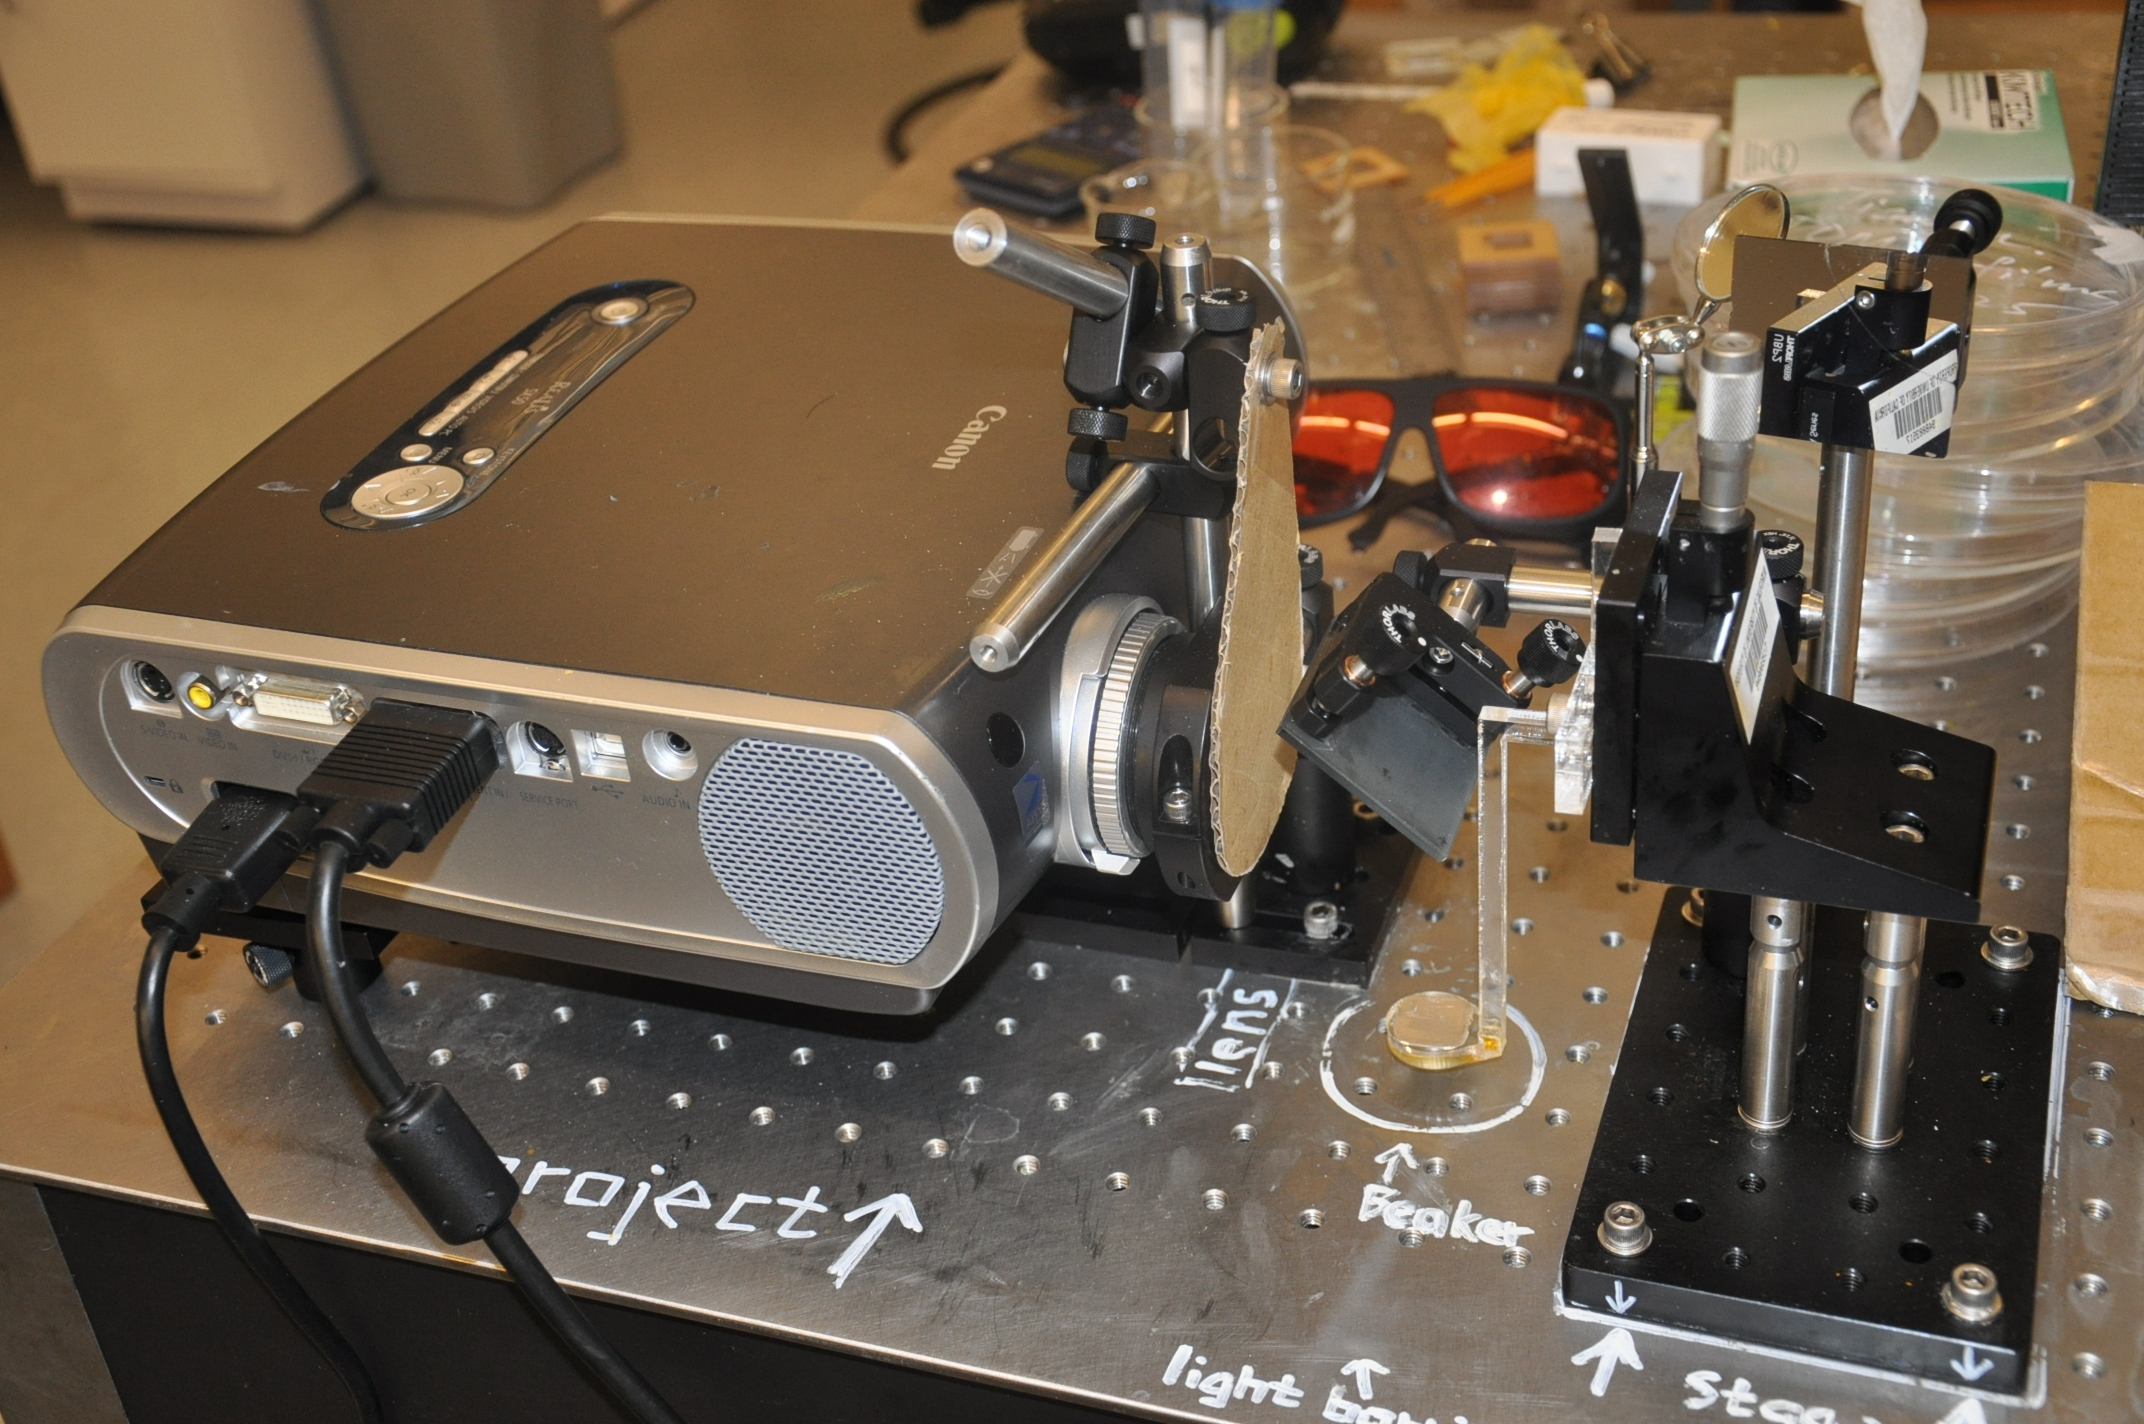
\includegraphics[width=400pt]{frontpic.jpg}
	\clearpage


	\raggedright

	\section{Device Introduction}\label{sec:device-introduction}
		The projection microstereolithography (P$\mu$SL) a novel freeform 3D micro-fabrication technology 
		which is capable of rapidly fabricating highly complex 3D microstructures in a layer-by-layer fashion. 
		This device use a digital data projector and simple optical components like a convex lens and a mirror. 
		Image will be projected on the photosensitive resin surface, polymerizing liquid resin into a desired 
		3D solid structure. \\ 
		\vspace{10pt}

		This device is a minimum system of projection micro stereolithography (P$\mu$SL) 3D-printer, adopting the
		technology from Howon Jove \footnote{http://www.jove.com/video/4457/micro-3d-printing-using-digital-projector-its-application-study-soft}.
		The devcie is with low resolution (about 200$\mu$m) but very easy operation and large printing area. 
		It's built for testing the characteristic of new materials like curing time, curing depth, fluidity and so on. \\
		\vspace{10pt}

		In this section, I will introduce the hardware, the software and the materials we used for the device. \\

		\vspace{20pt}

		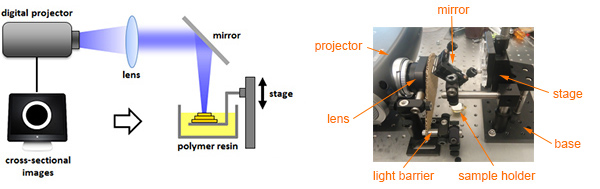
\includegraphics[width=\textwidth]{main.jpg}

		\subsection{Hardware}\label{sec:hardware}
		 \vspace{10pt}

			\subsubsection{projector}\label{sec:projector}
			 \begin{tabularx}{\textwidth}{ cX }
				\raisebox{-0.9\height}{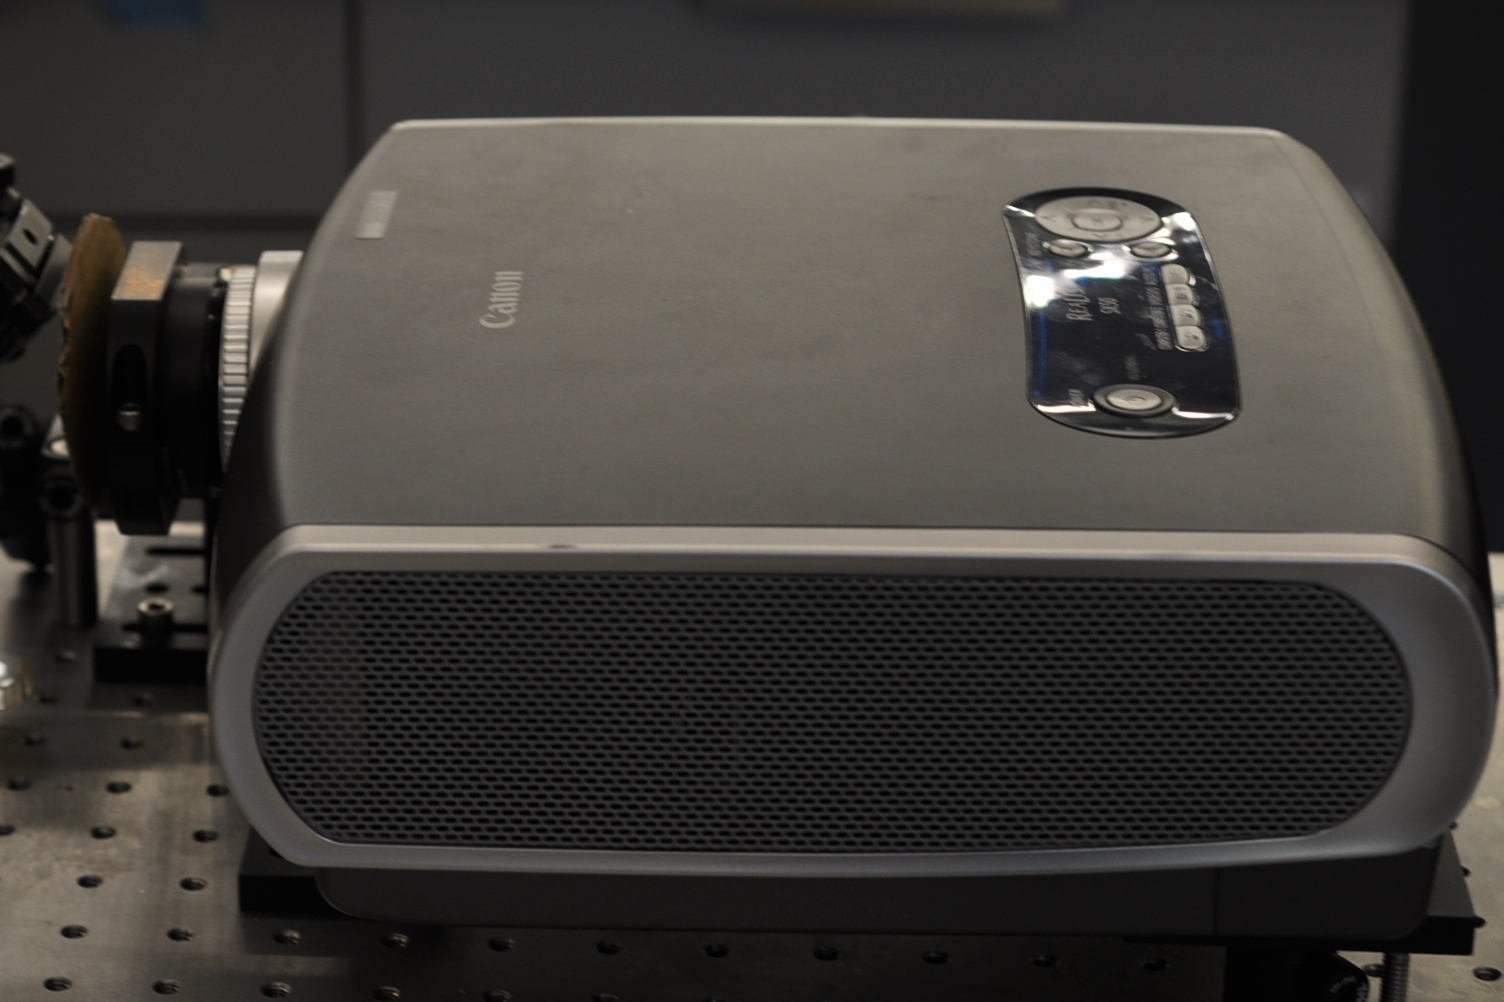
\includegraphics[width=0.33\textwidth]{intro1-1-1.jpg}} &
			 	The projector is core part of the device. It is connected to the computer and the 
			 	desktop background will be projected out. Just change the background when you want to be project different 
			 	images. \textbf{Push the power button} to turn on the projector and \textbf{double-push} to turn it off. 
			 	\textbf{Rotating the ring} on the projector lens can adjusting the focial length and making the image sharper. 
			 \end{tabularx}

			\subsubsection{Convex Lens}\label{sec:convex-lens}
			 \begin{tabularx}{\textwidth}{ cX }
				\raisebox{-0.9\height}{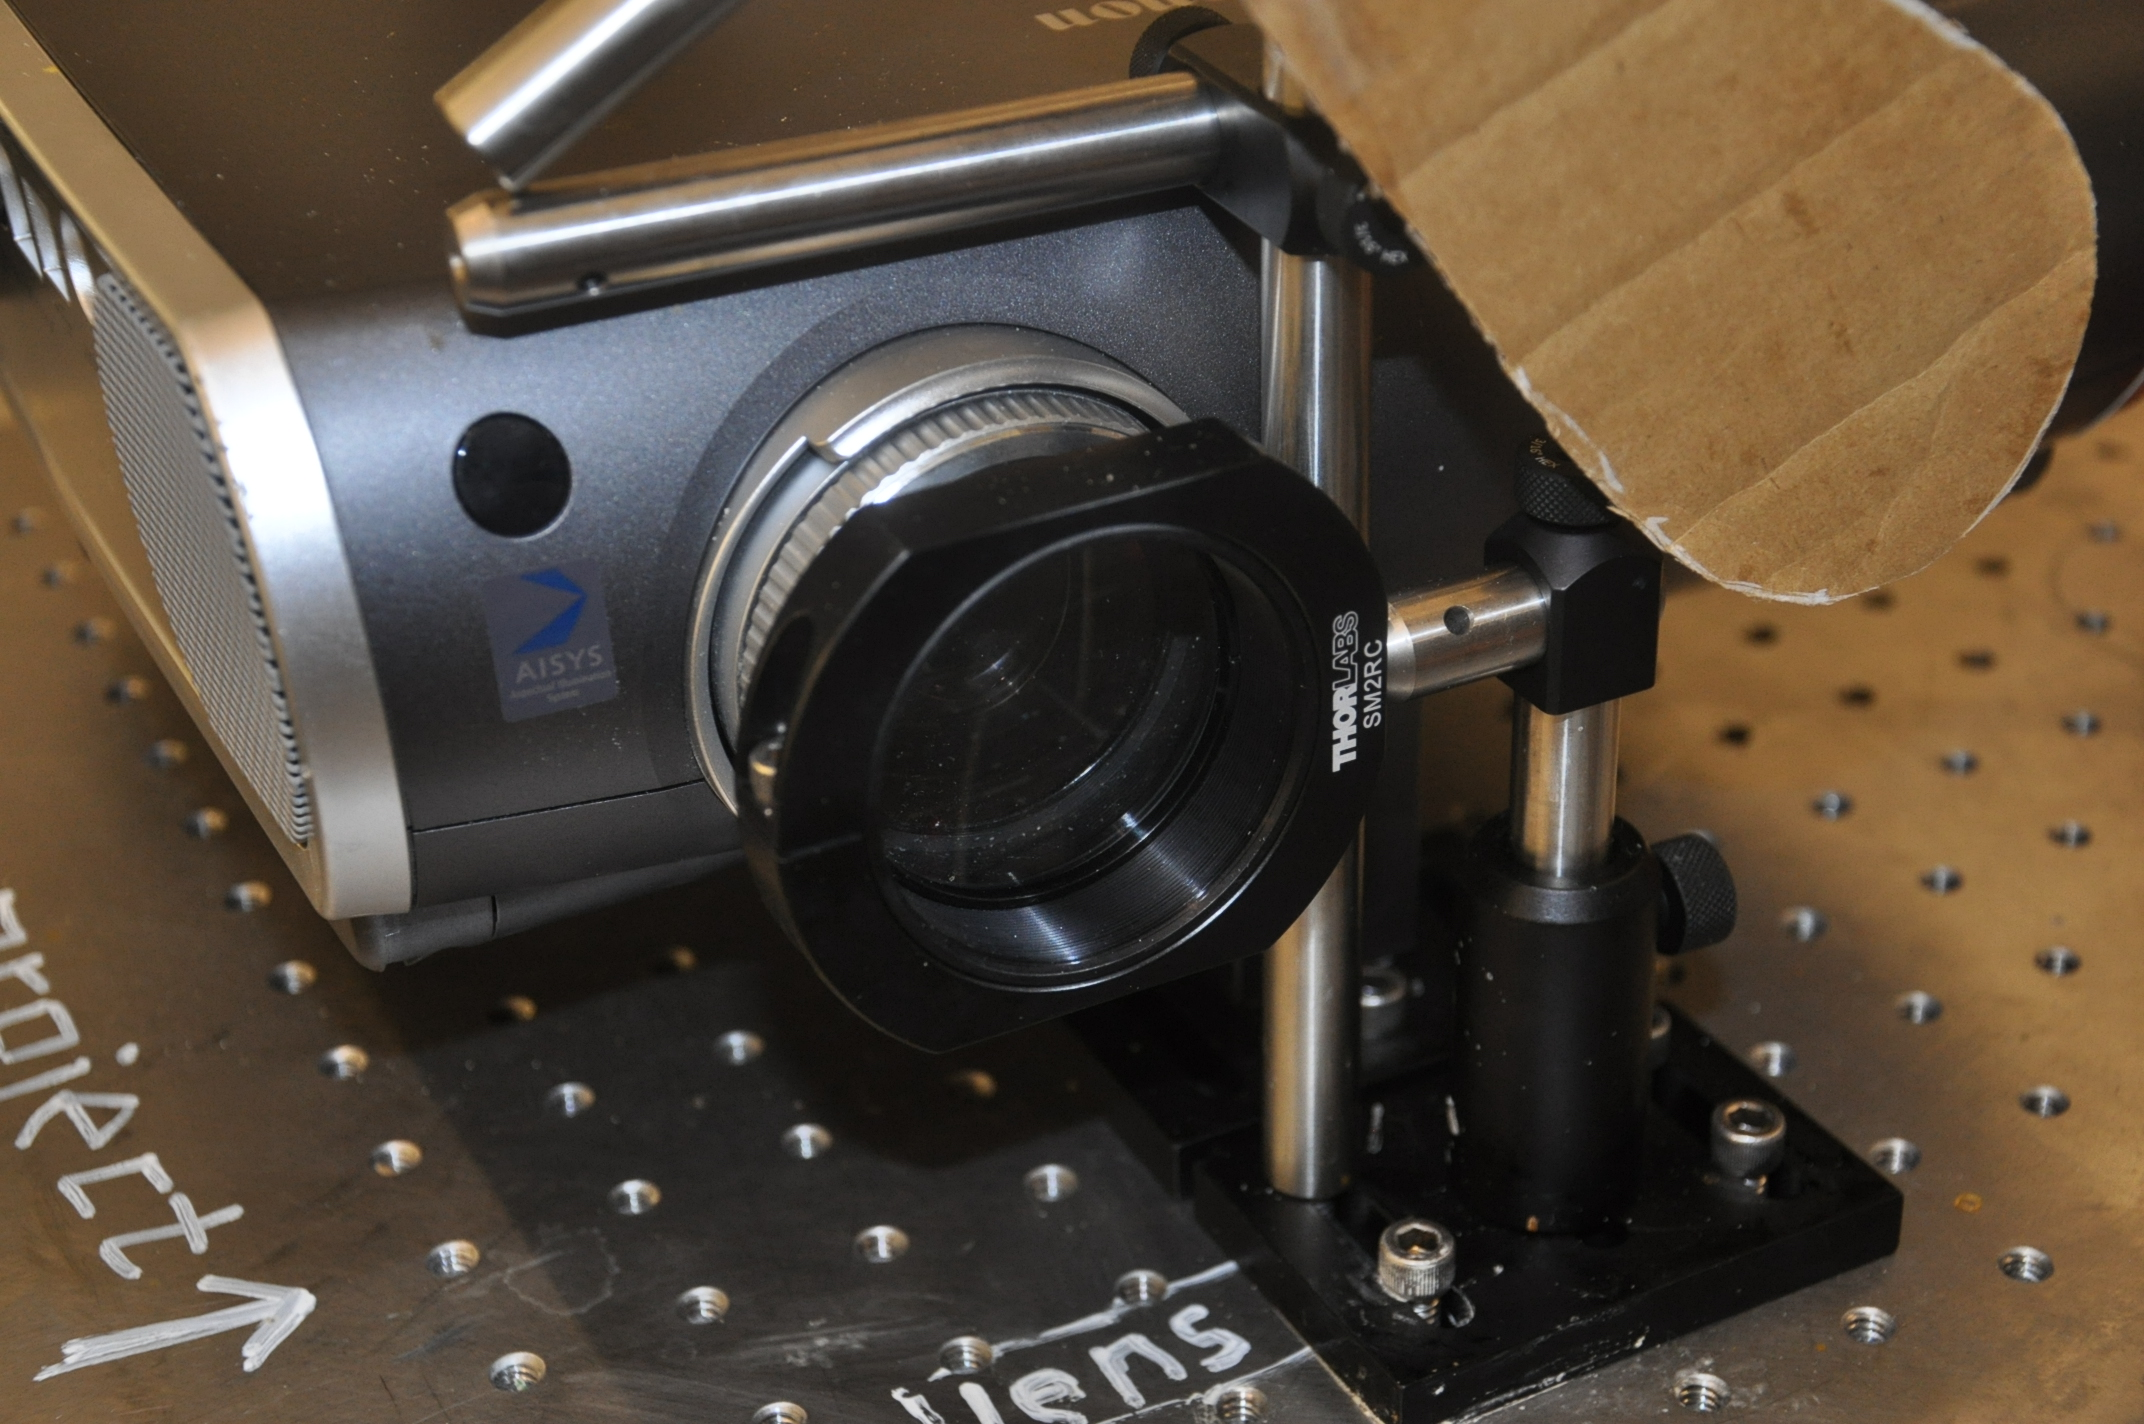
\includegraphics[width=0.33\textwidth]{intro1-1-2.jpg}} &
			 	The convex lens is used to decrease the projected image as well as shorten the image distance. 
			 	Then image is able to projected on the sample holder fix on the linear stage next to the projector. 
			 	A light barrier is set in front of the lens. It's used to block the optical path.
			 	As the convex lens is well adjusted, it's strongly adviced not to adjust it again in general use. But if 
			 	you have to, please see the appendix at the end of this manual.
			 \end{tabularx}
			 \vspace{30pt}

			\subsubsection{Mirror}\label{sec:mirror}
			 \begin{tabularx}{\textwidth}{ cX }
				\raisebox{-0.9\height}{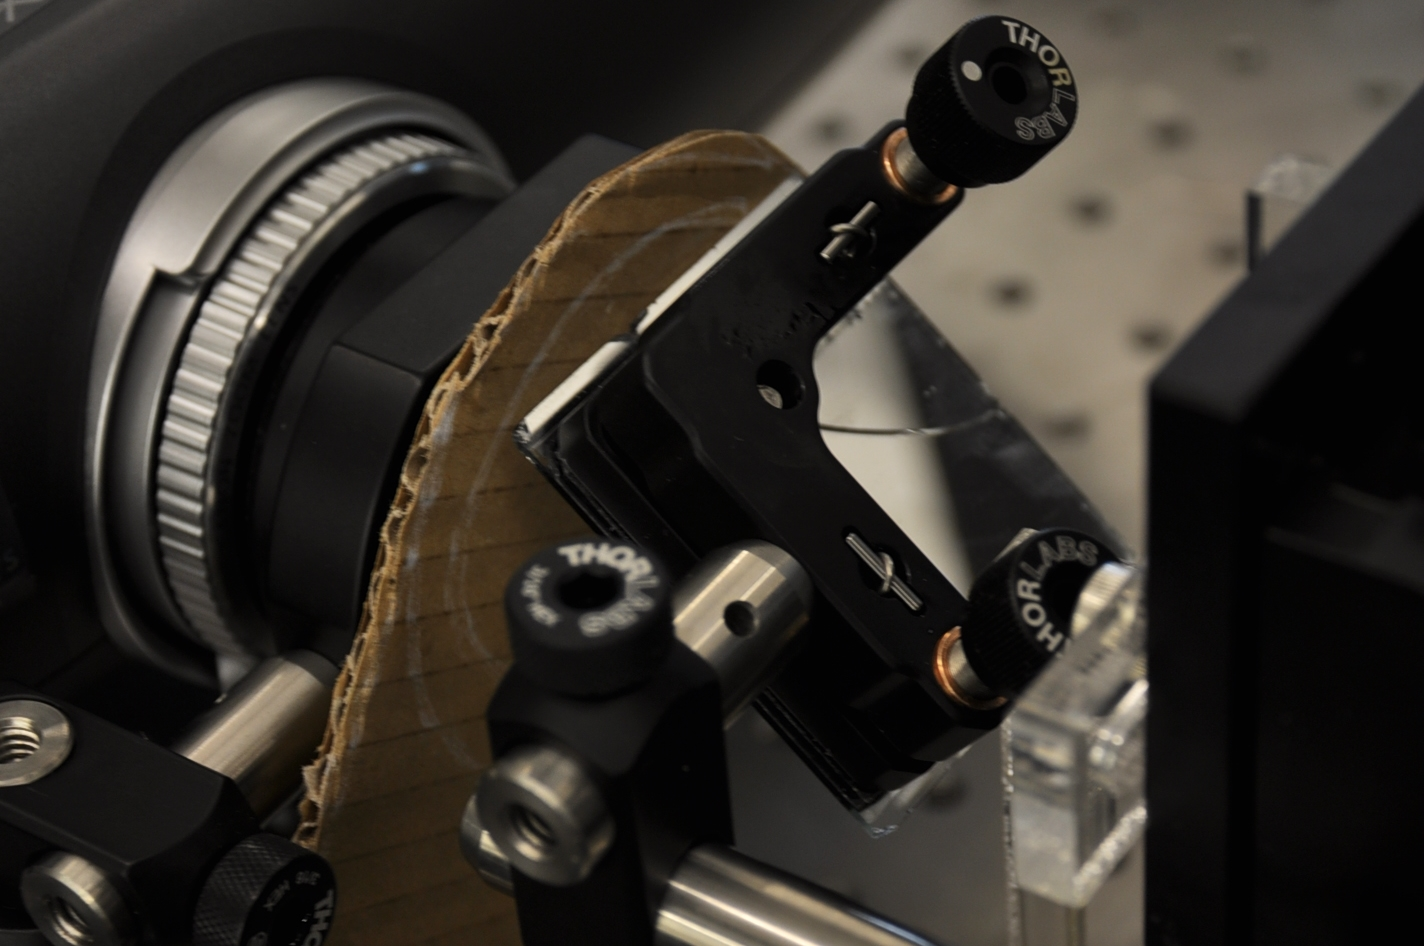
\includegraphics[width=0.33\textwidth]{intro1-1-3.jpg}} &
			 	The mirror rotate the main optical axis and let the image be just pojected on the sample 
			 	holder. Note that the mirror should be placed in a specific distance in front of the lens. More details 
			 	about this will be introduce in section 1.1.4. If you have to adjust the mirror, please see the appendix.
			 \end{tabularx}

			\subsubsection{Linear Stage}\label{sec:linear-stage}
			 \begin{tabularx}{\textwidth}{ cX }
				\raisebox{-0.9\height}{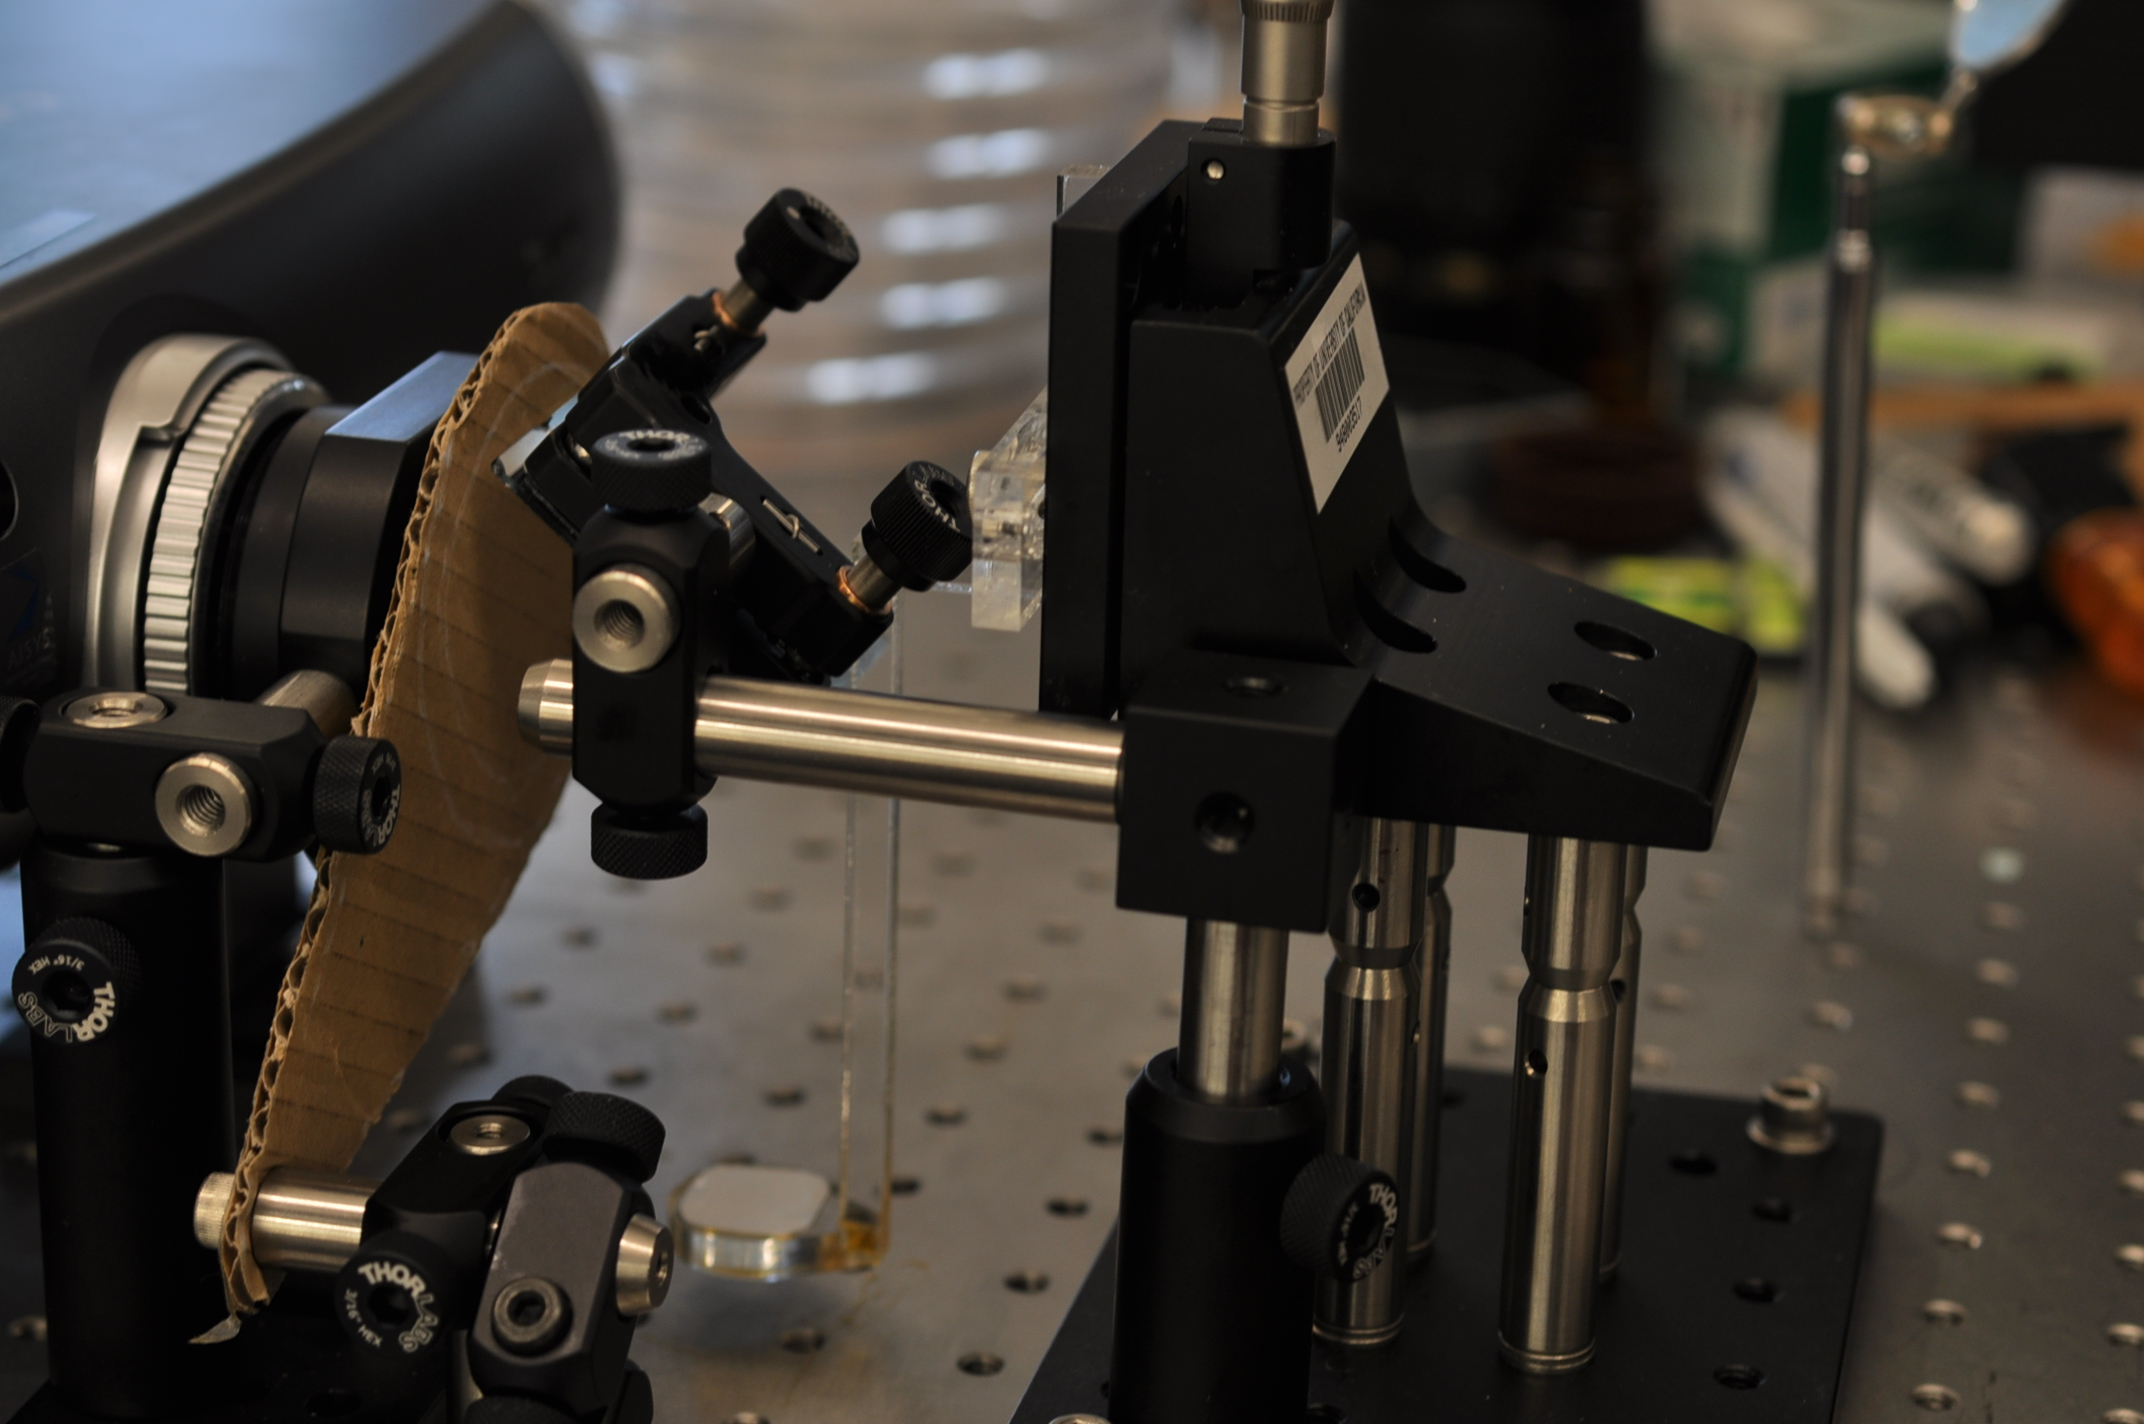
\includegraphics[width=0.33\textwidth]{intro1-1-4.jpg}} &
			 	The linear stage is also one of the most important part. There's a sample holder fixed on it. Rotate 
			 	the knob clockwise can lower the stage and counterclockwise upper the stage. 

			 	// TODO need to expand	

			 	The \textbf{stage assembly} is \textit{stage} + \textit{base} + \textit{sample holder} + \textit{mirror}.

			 \end{tabularx}
			 \vspace{10pt}

        \subsection{Software}\label{sec:software}             
        	The portable printer actually do not need any softwares because it meant to be operated manually. But there
        	are still some works on computer.

		\begin{itemize}              
			\item When you need to \textbf{change the projecter's image output}, you should change the desktop background of the 
			computer by \textbf{right click - set background}.
		\end{itemize}

			\begin{tabularx}{\textwidth}{ XXX }
			 \raisebox{-\height}{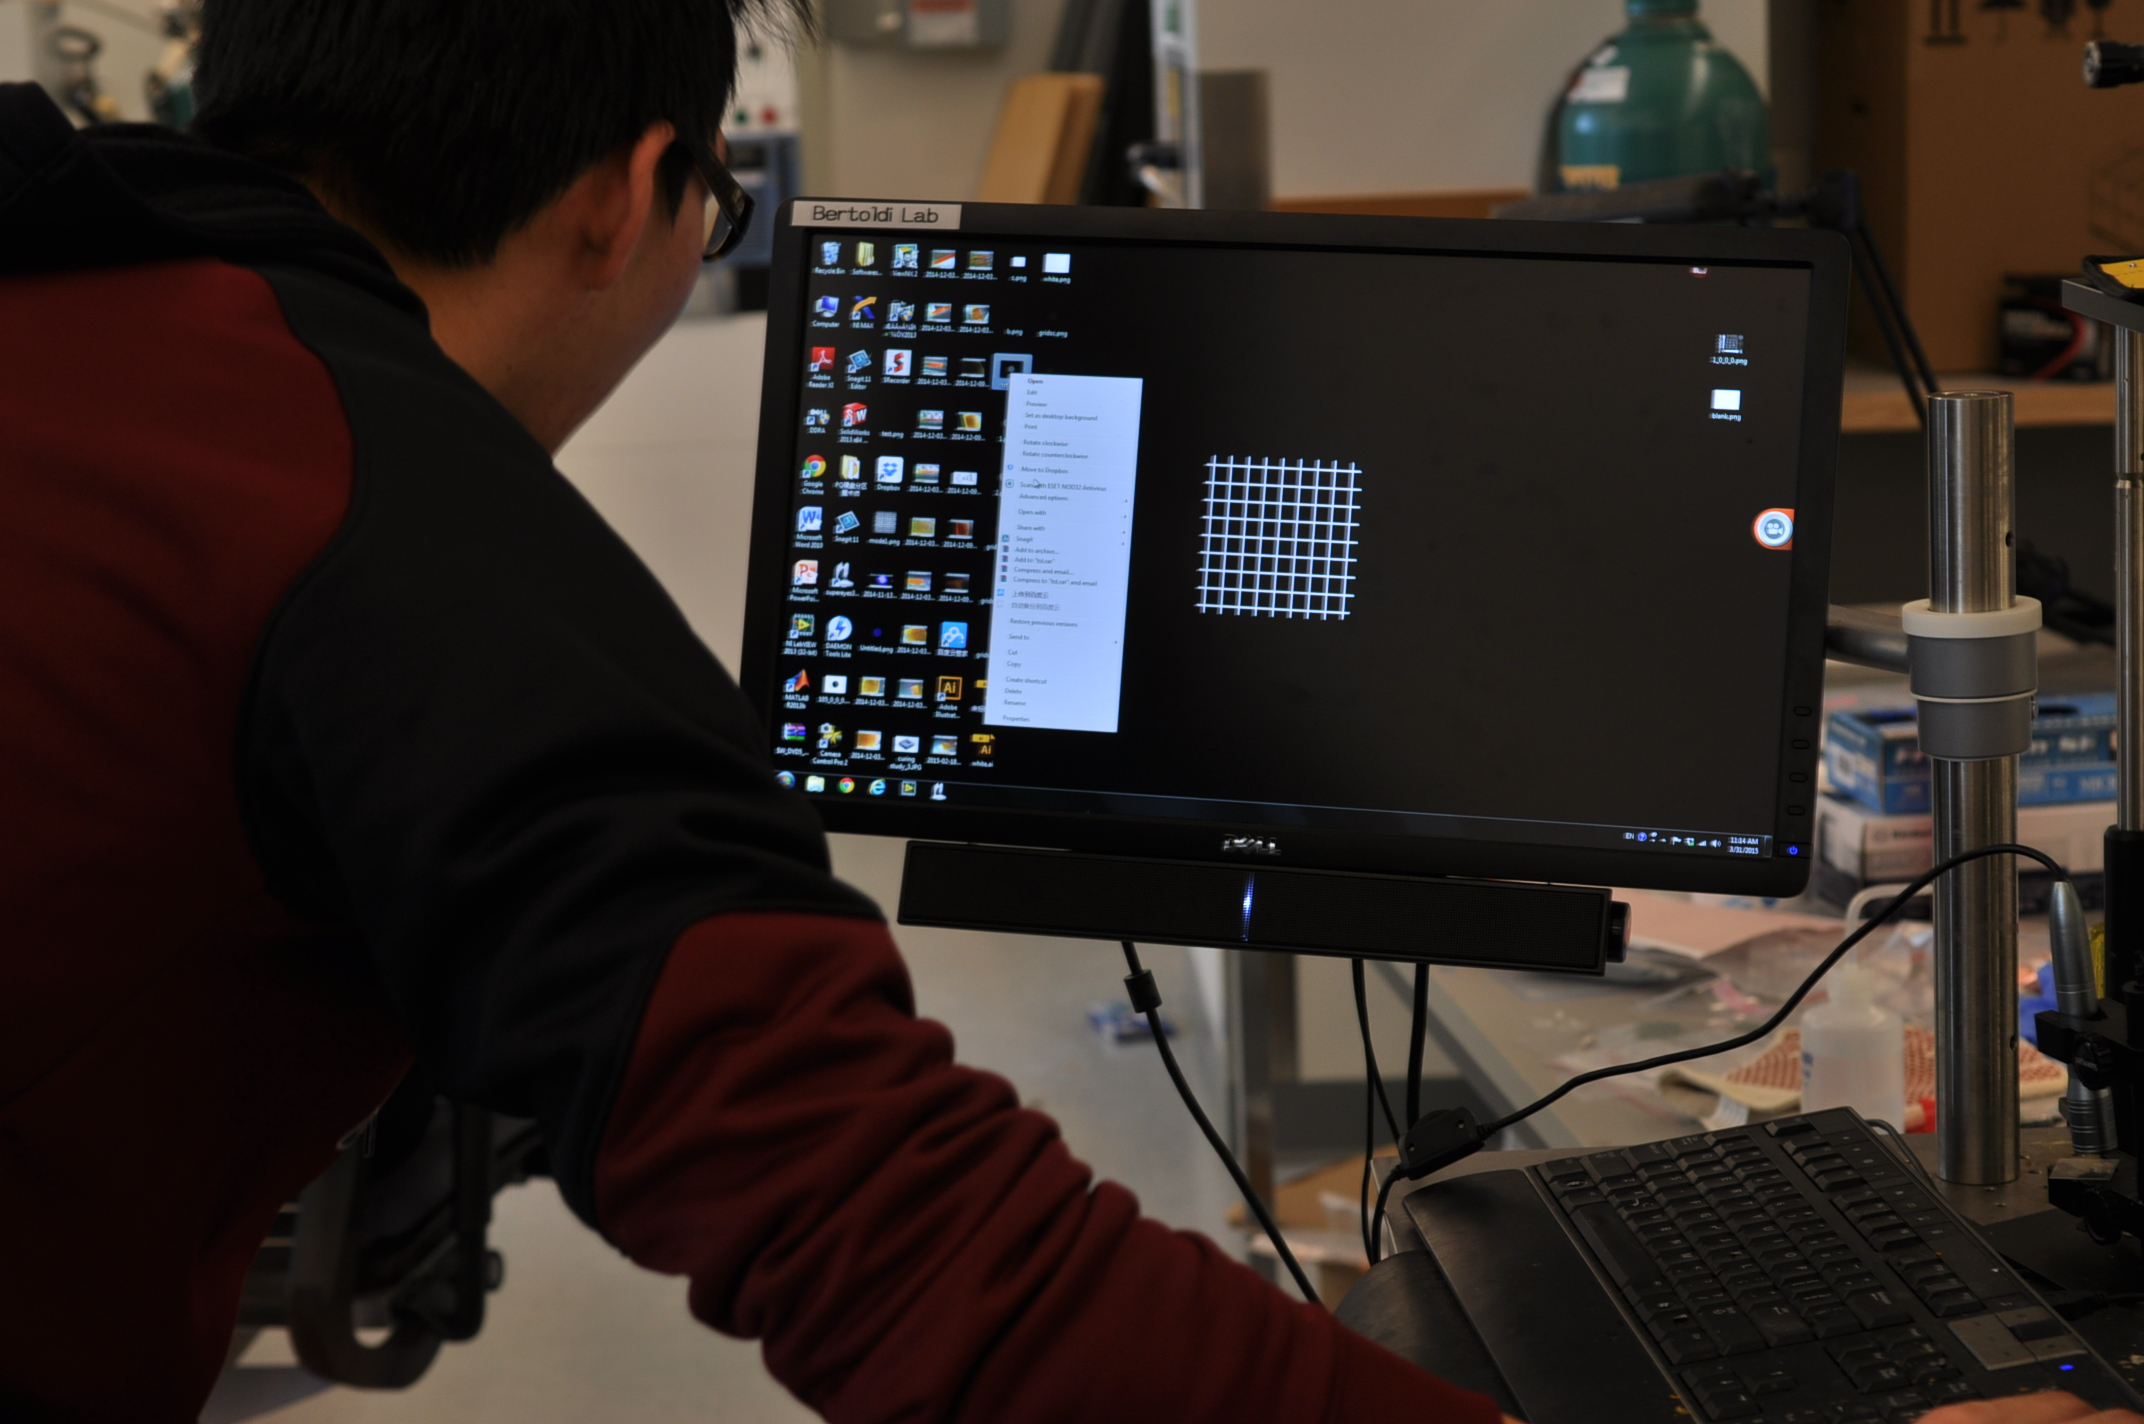
\includegraphics[width=0.3\textwidth]{software1_2.jpg}}
				&\raisebox{-\height}{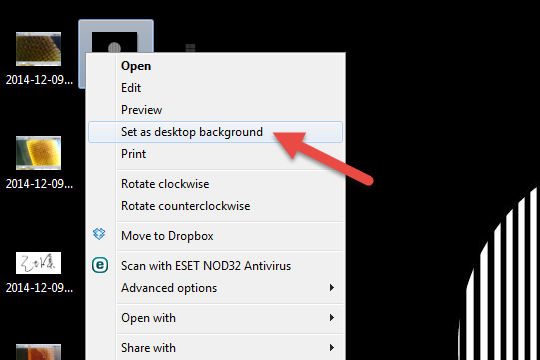
\includegraphics[width=0.3\textwidth]{software1_1.png}}
			 	&\raisebox{-\height}{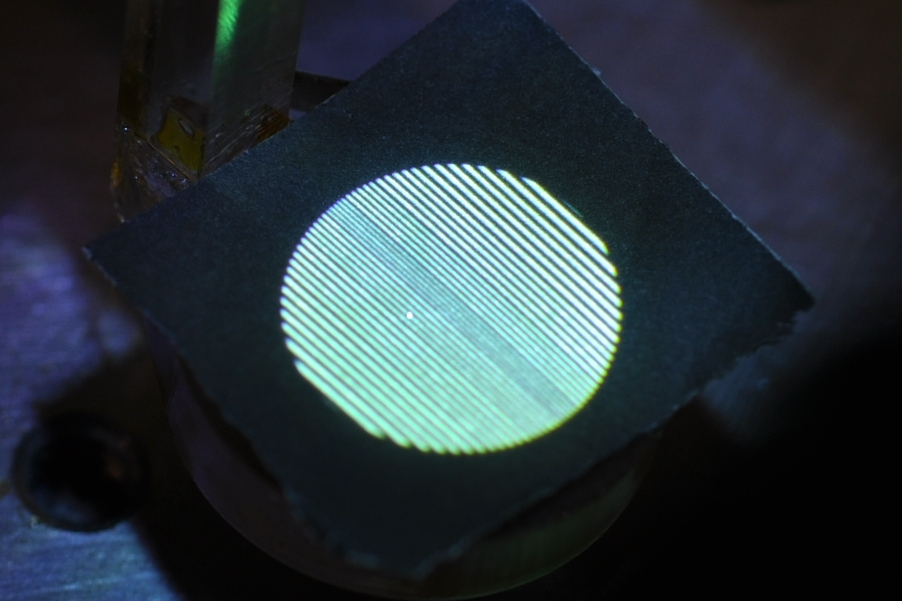
\includegraphics[width=0.3\textwidth]{pre4r.jpg}}\\
			 	\\
			\end{tabularx}

            \begin{itemize}              
				\item \textbf{An python program is written to help with the operation}. It can give out vocal instructions to assist 
	            you to do the right action at the right time. Four parameters should be set everytime you open the program. The 
	            \textit{number of layers} you need to print (depends on the height of sample and each layer), the \textit
	            {thickness of each layer}, the \textit{first layer curing time}, the \textit{other layers curing time} (both need to 
	            be tested with different materials and also depend on the cross-linking density you need) and the \textit{fluid 
	            flowing time} (depends on the fluidity of the material, should be set long enough for the material liquid level 
	            covering the whole sample within this time). \\              
	            After you finishing inputing the parameters, the vocal assistance will start in 10 seconds.             
	         \end{itemize}

			\begin{tabularx}{\textwidth}{ XXX }
			 	\raisebox{-\height}{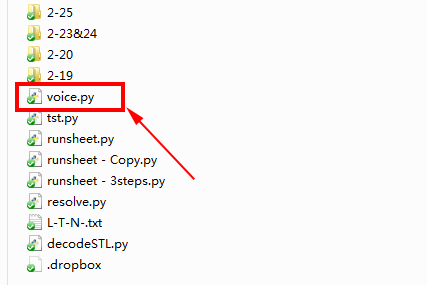
\includegraphics[width=0.3\textwidth]{voice_folder.png}}
				&\raisebox{-\height}{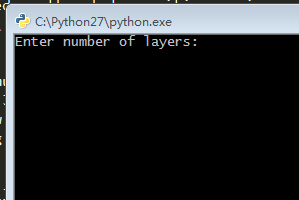
\includegraphics[width=0.3\textwidth]{voice_interface.png}}
			 	&\raisebox{-\height}{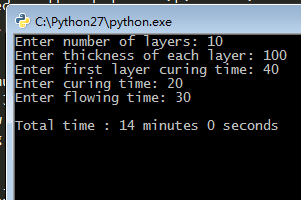
\includegraphics[width=0.3\textwidth]{voice_interface2.png}}\\
			 	\\
			\end{tabularx}

			

		\subsection{Materials}\label{sec:materials}
			// TODO
			\vspace{50pt}


	\section{Normal Operation Procedure}\label{sec:page-layout}
	In this section, I will introduce the normal operation precedure for the 3d-printer. Just follow the steps. \\
	\textbf {To your own safety, always wear gloves before doing anything and wash hands after experiments.}

		\subsection{Preperation}\label{sec:preperation}

		 \begin{itemize}
		  \begin{tabularx}{\textwidth}{ XXX }
		   \item \textbf{Step 1} : Put the stage in right place. The mirror shall be about $\sim\frac{1}{2}$ inch 
		   	in front of the lens. Also make sure that the screws on corners are embedded into the holes on the table.
		 	&\raisebox{-\height}{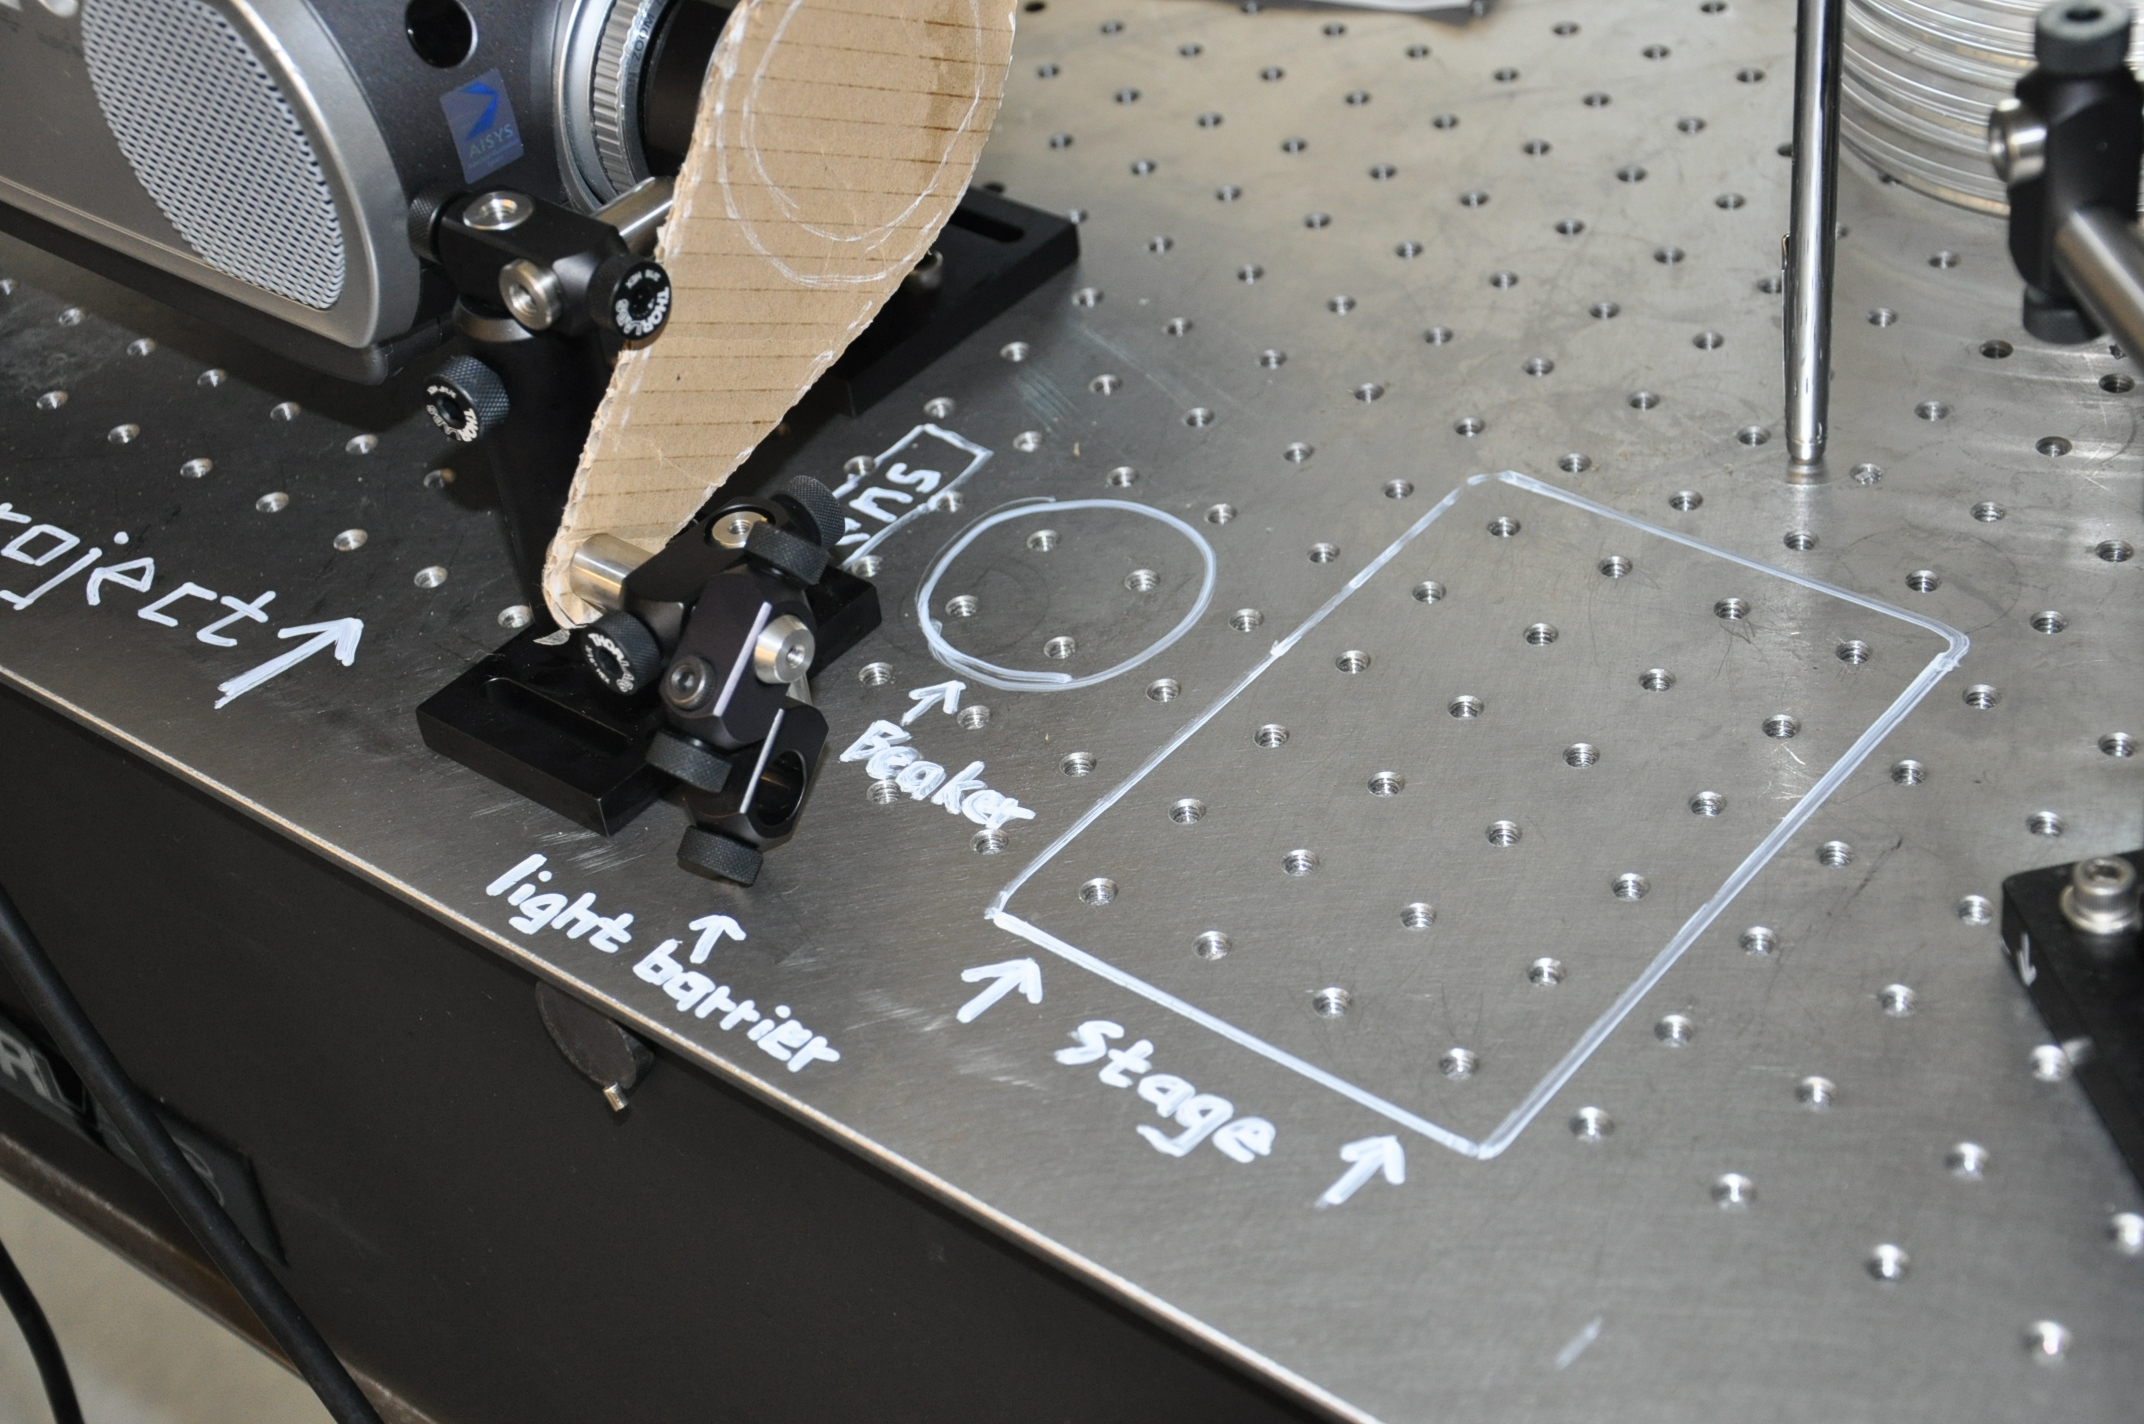
\includegraphics[width=0.3\textwidth]{pre2l.jpg}}
		 	&\raisebox{-\height}{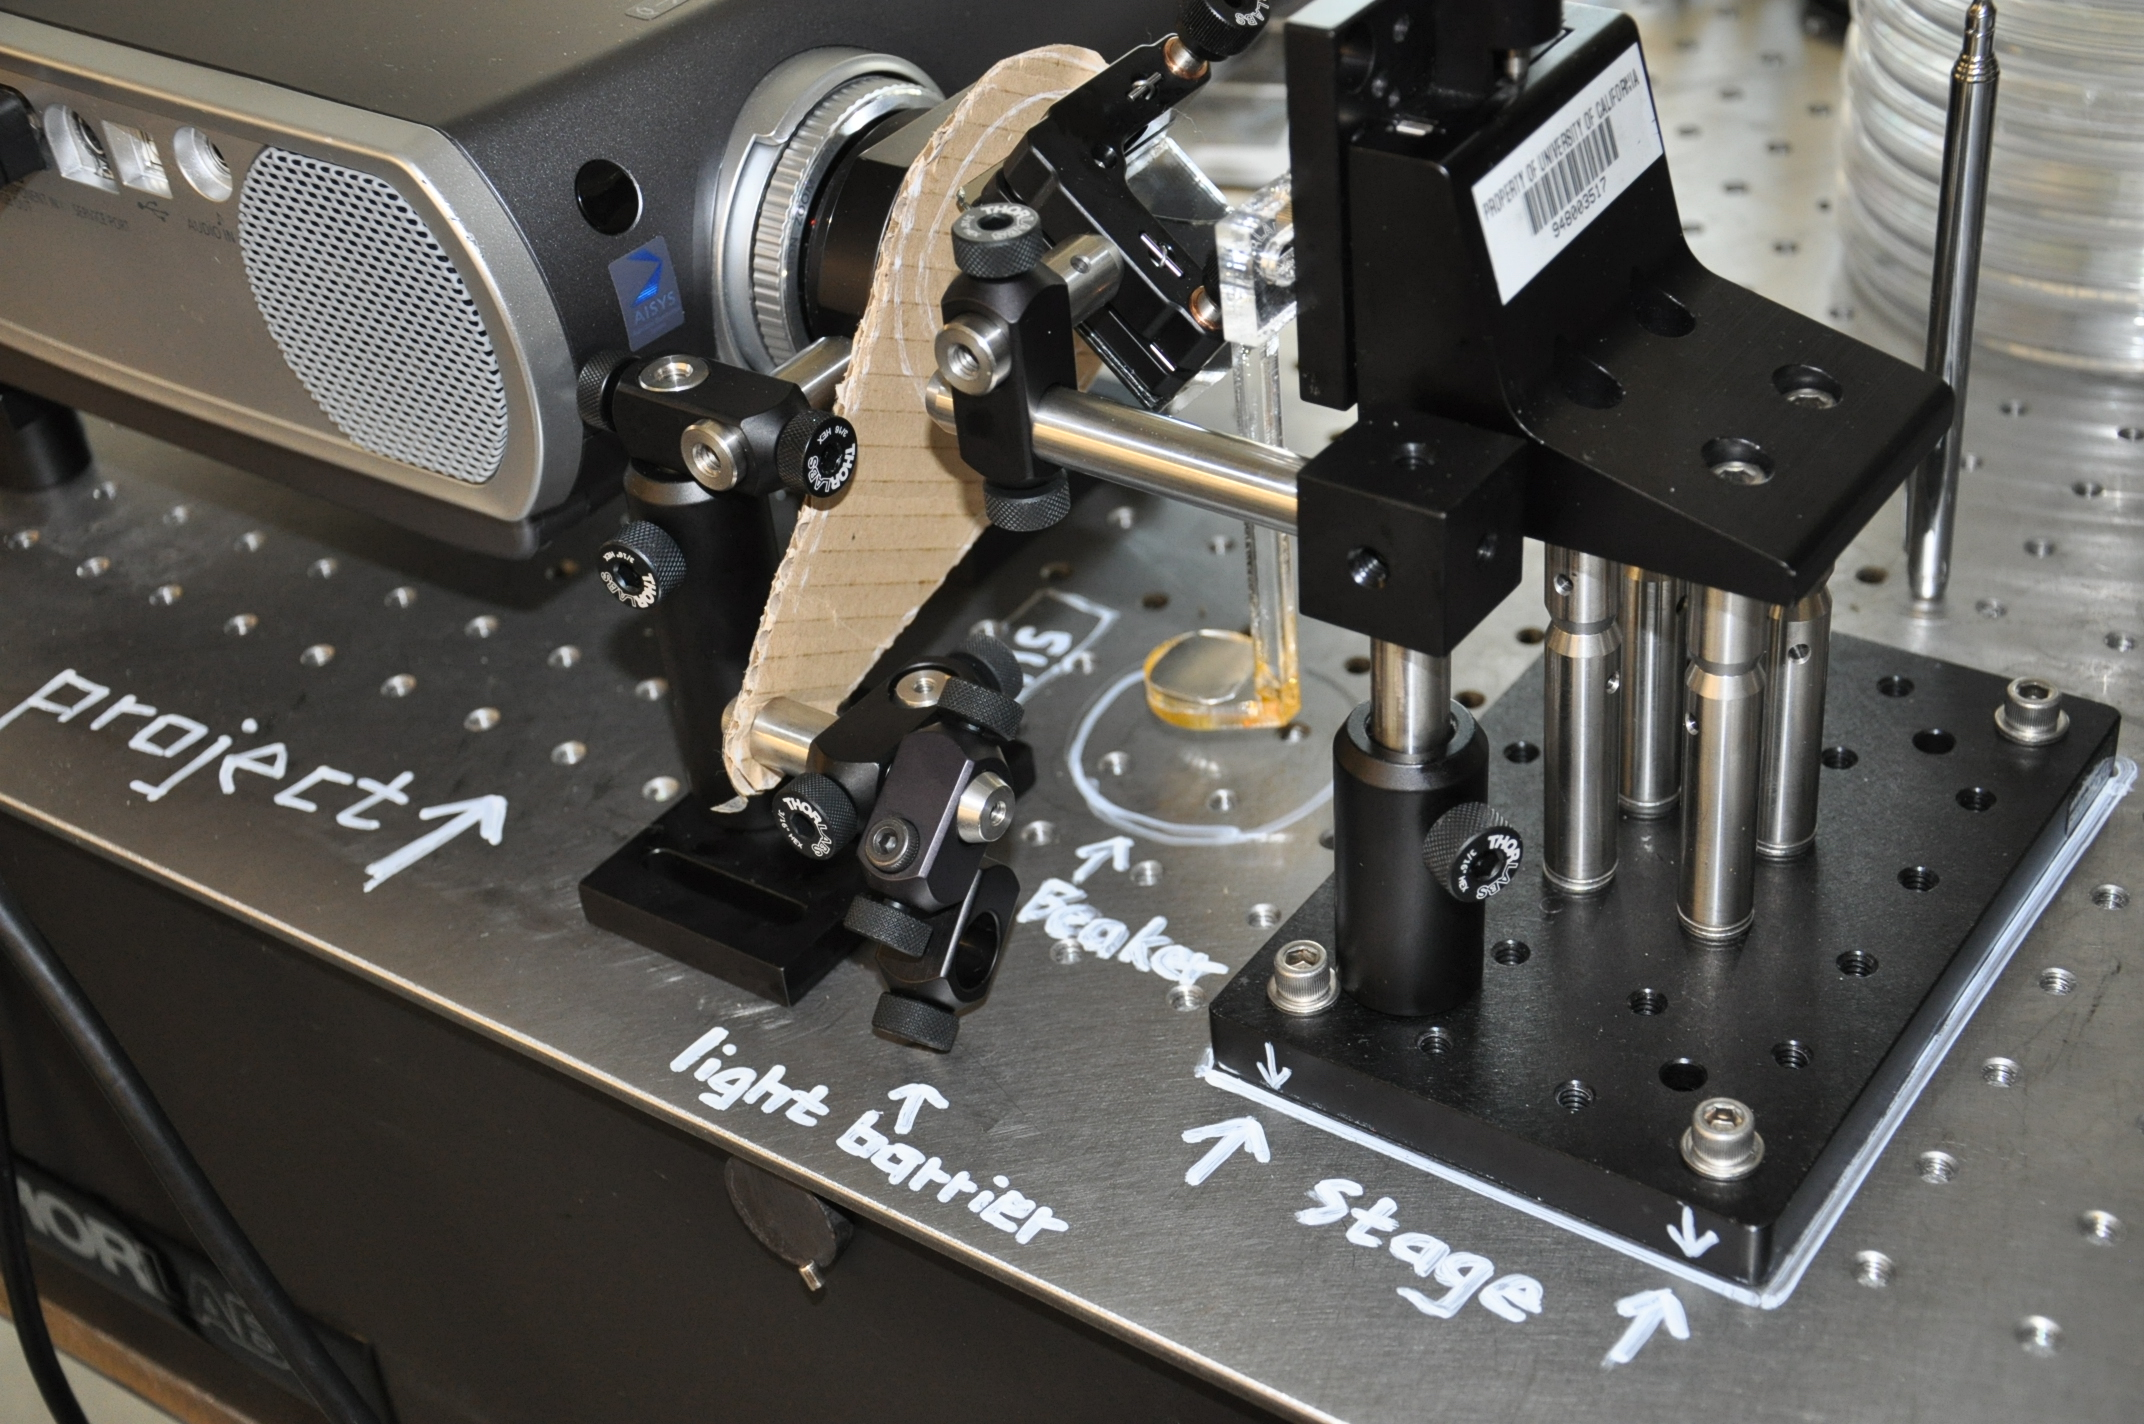
\includegraphics[width=0.3\textwidth]{pre2r.jpg}}\\
		 	\\
		  \end{tabularx}

		  \begin{tabularx}{\textwidth}{ XXX }
		   \item \textbf{Step 2} : Check the position of linear stage. Make sure that the inital position is 5mm 
			as shown in picture.
		 	&\raisebox{-\height}{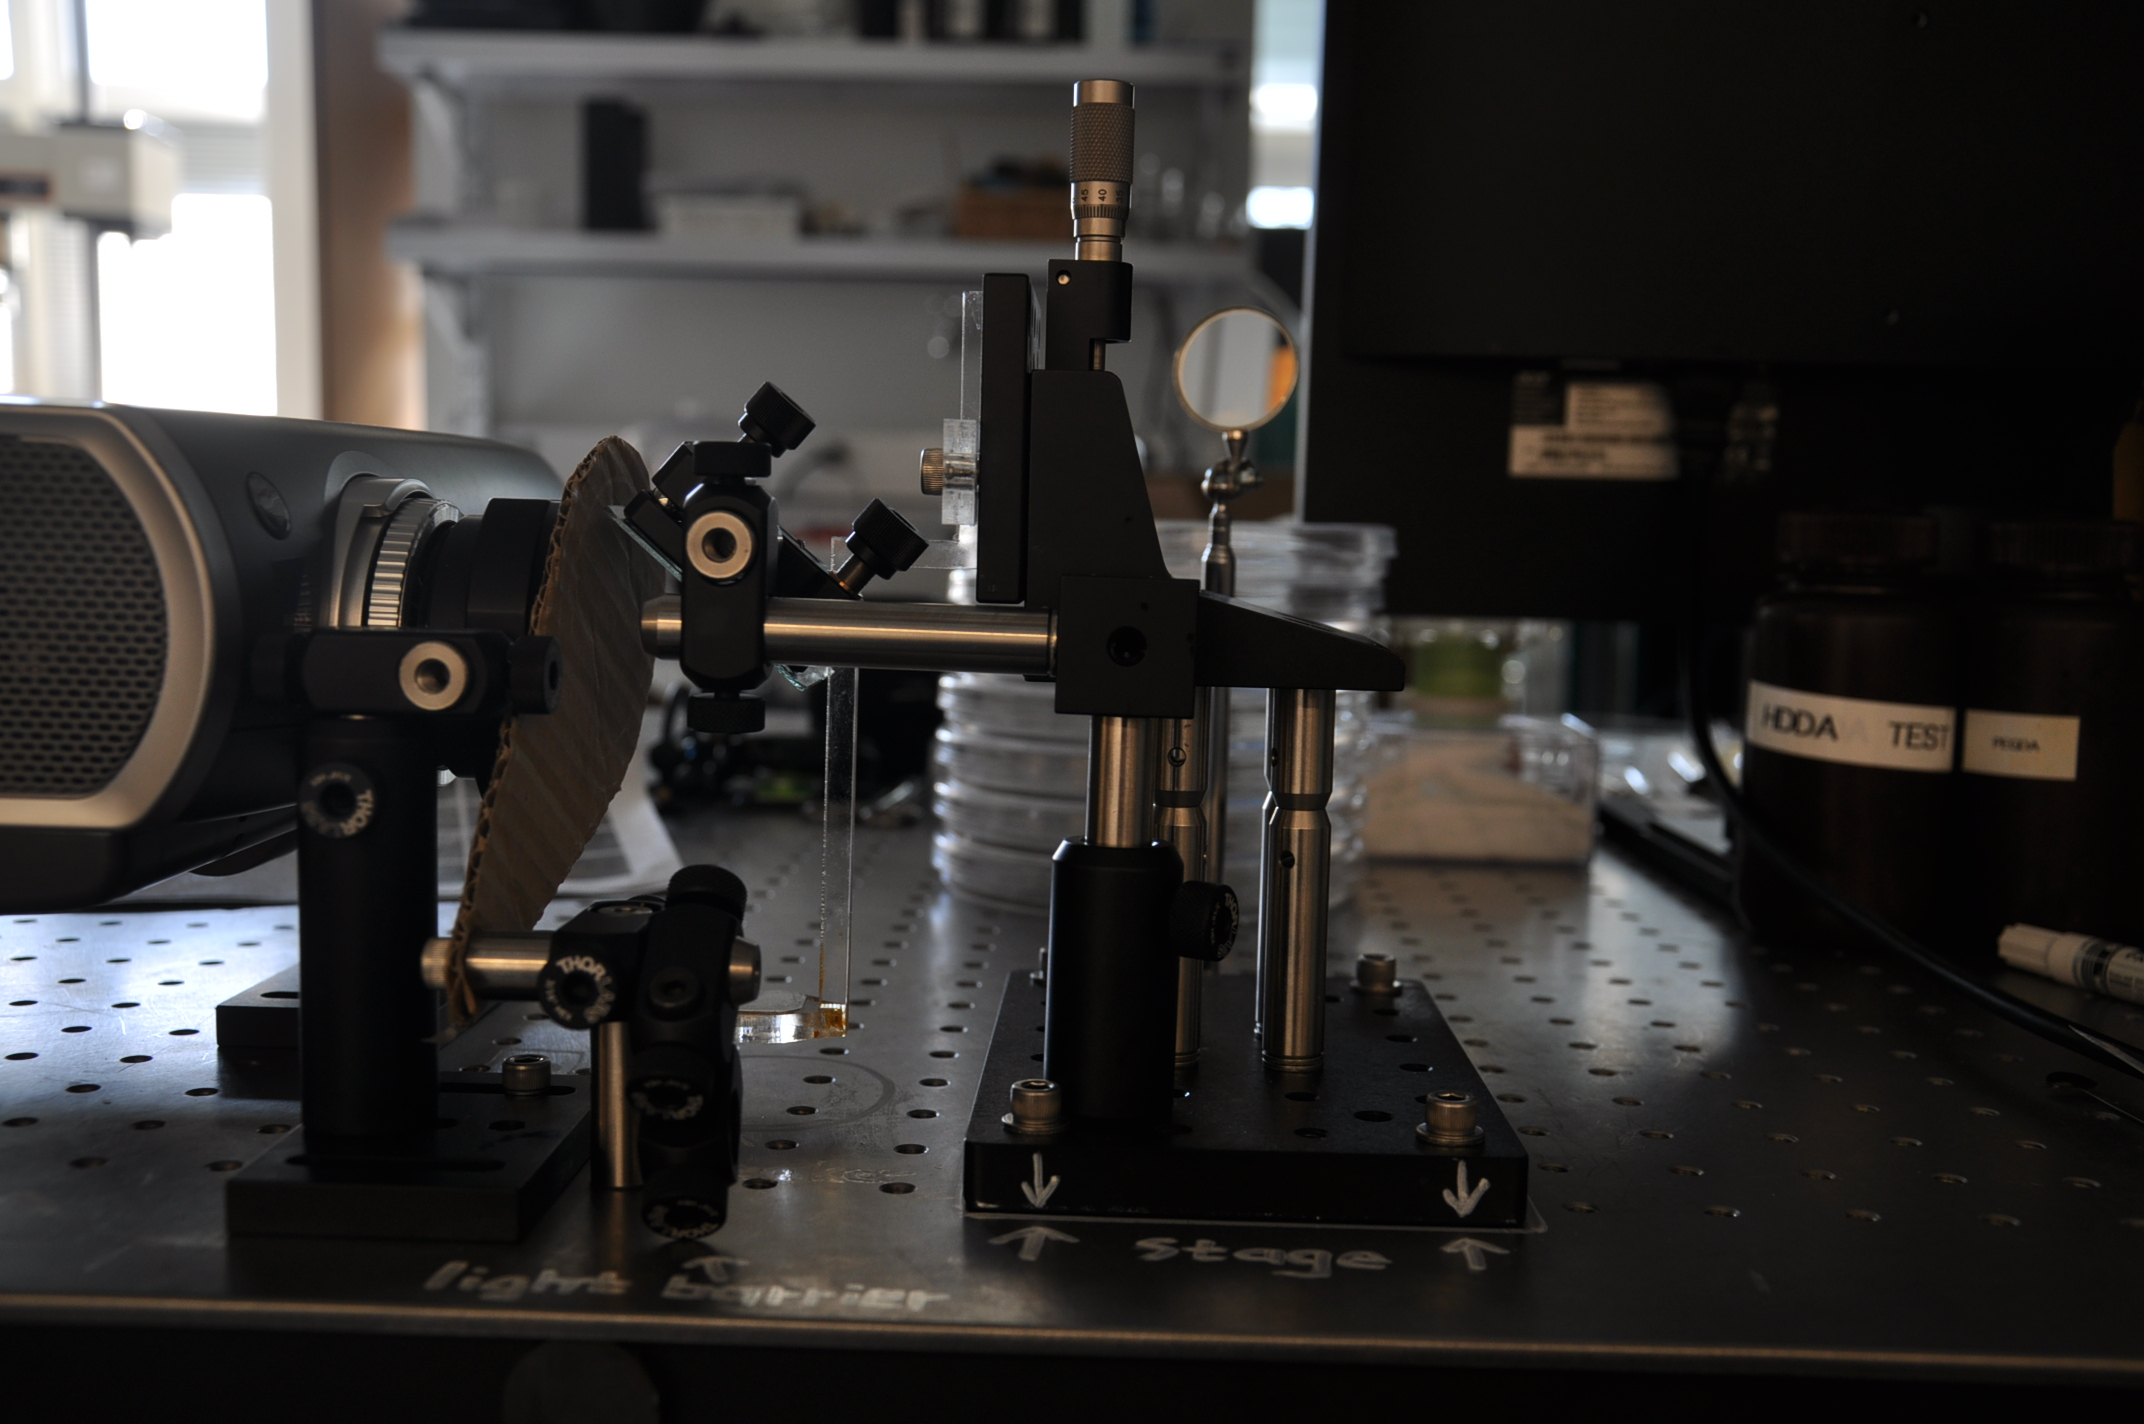
\includegraphics[width=0.3\textwidth]{pre1l.jpg}}
		 	&\raisebox{-\height}{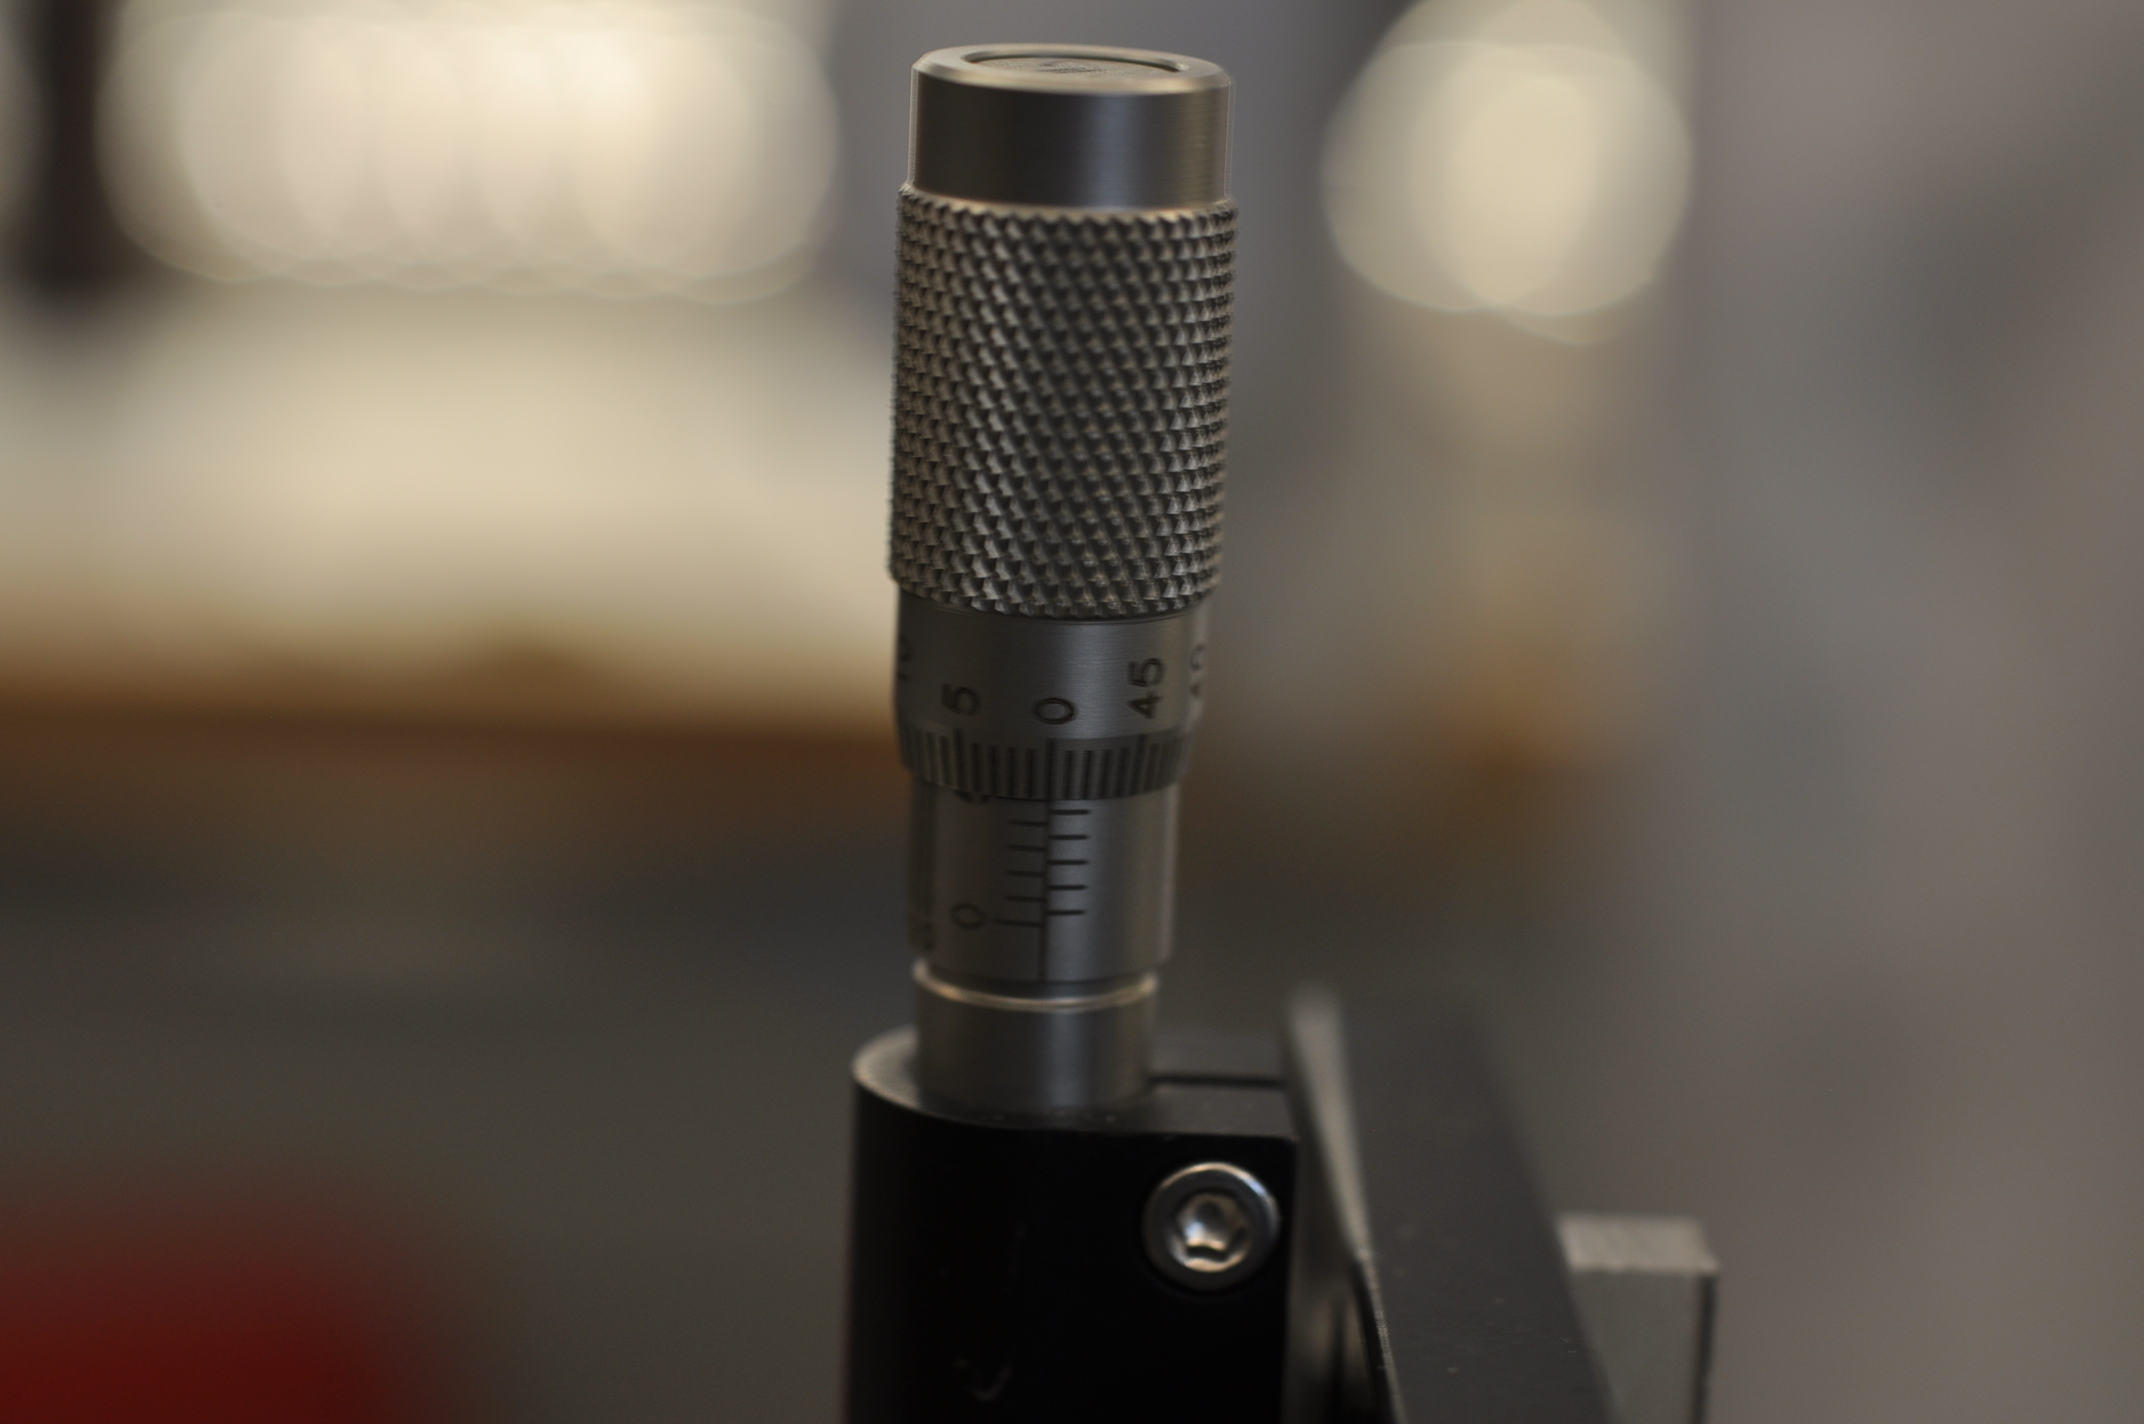
\includegraphics[width=0.3\textwidth]{pre1r.jpg}}\\
		 	\\
		  \end{tabularx}

		  \begin{tabularx}{\textwidth}{ XXX }
		   \item \textbf{Step 3} : Now \textbf{open} the computer. \textbf{Set} 'tst.png' as desktop background. \textbf{Turn on} 
		   the projector and \textbf{open} the light barrier by rotating it.
		 	&\raisebox{-\height}{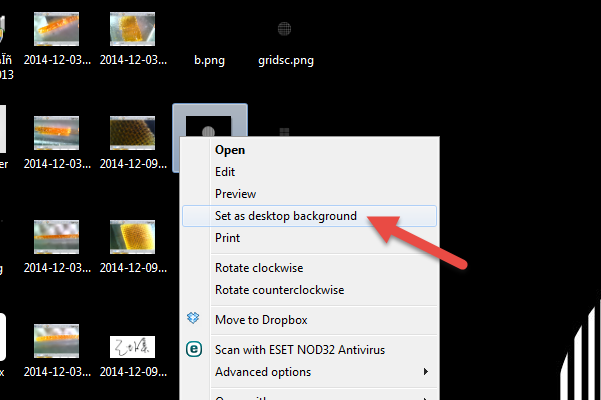
\includegraphics[width=0.3\textwidth]{pre3r.png}}
		 	&\raisebox{-\height}{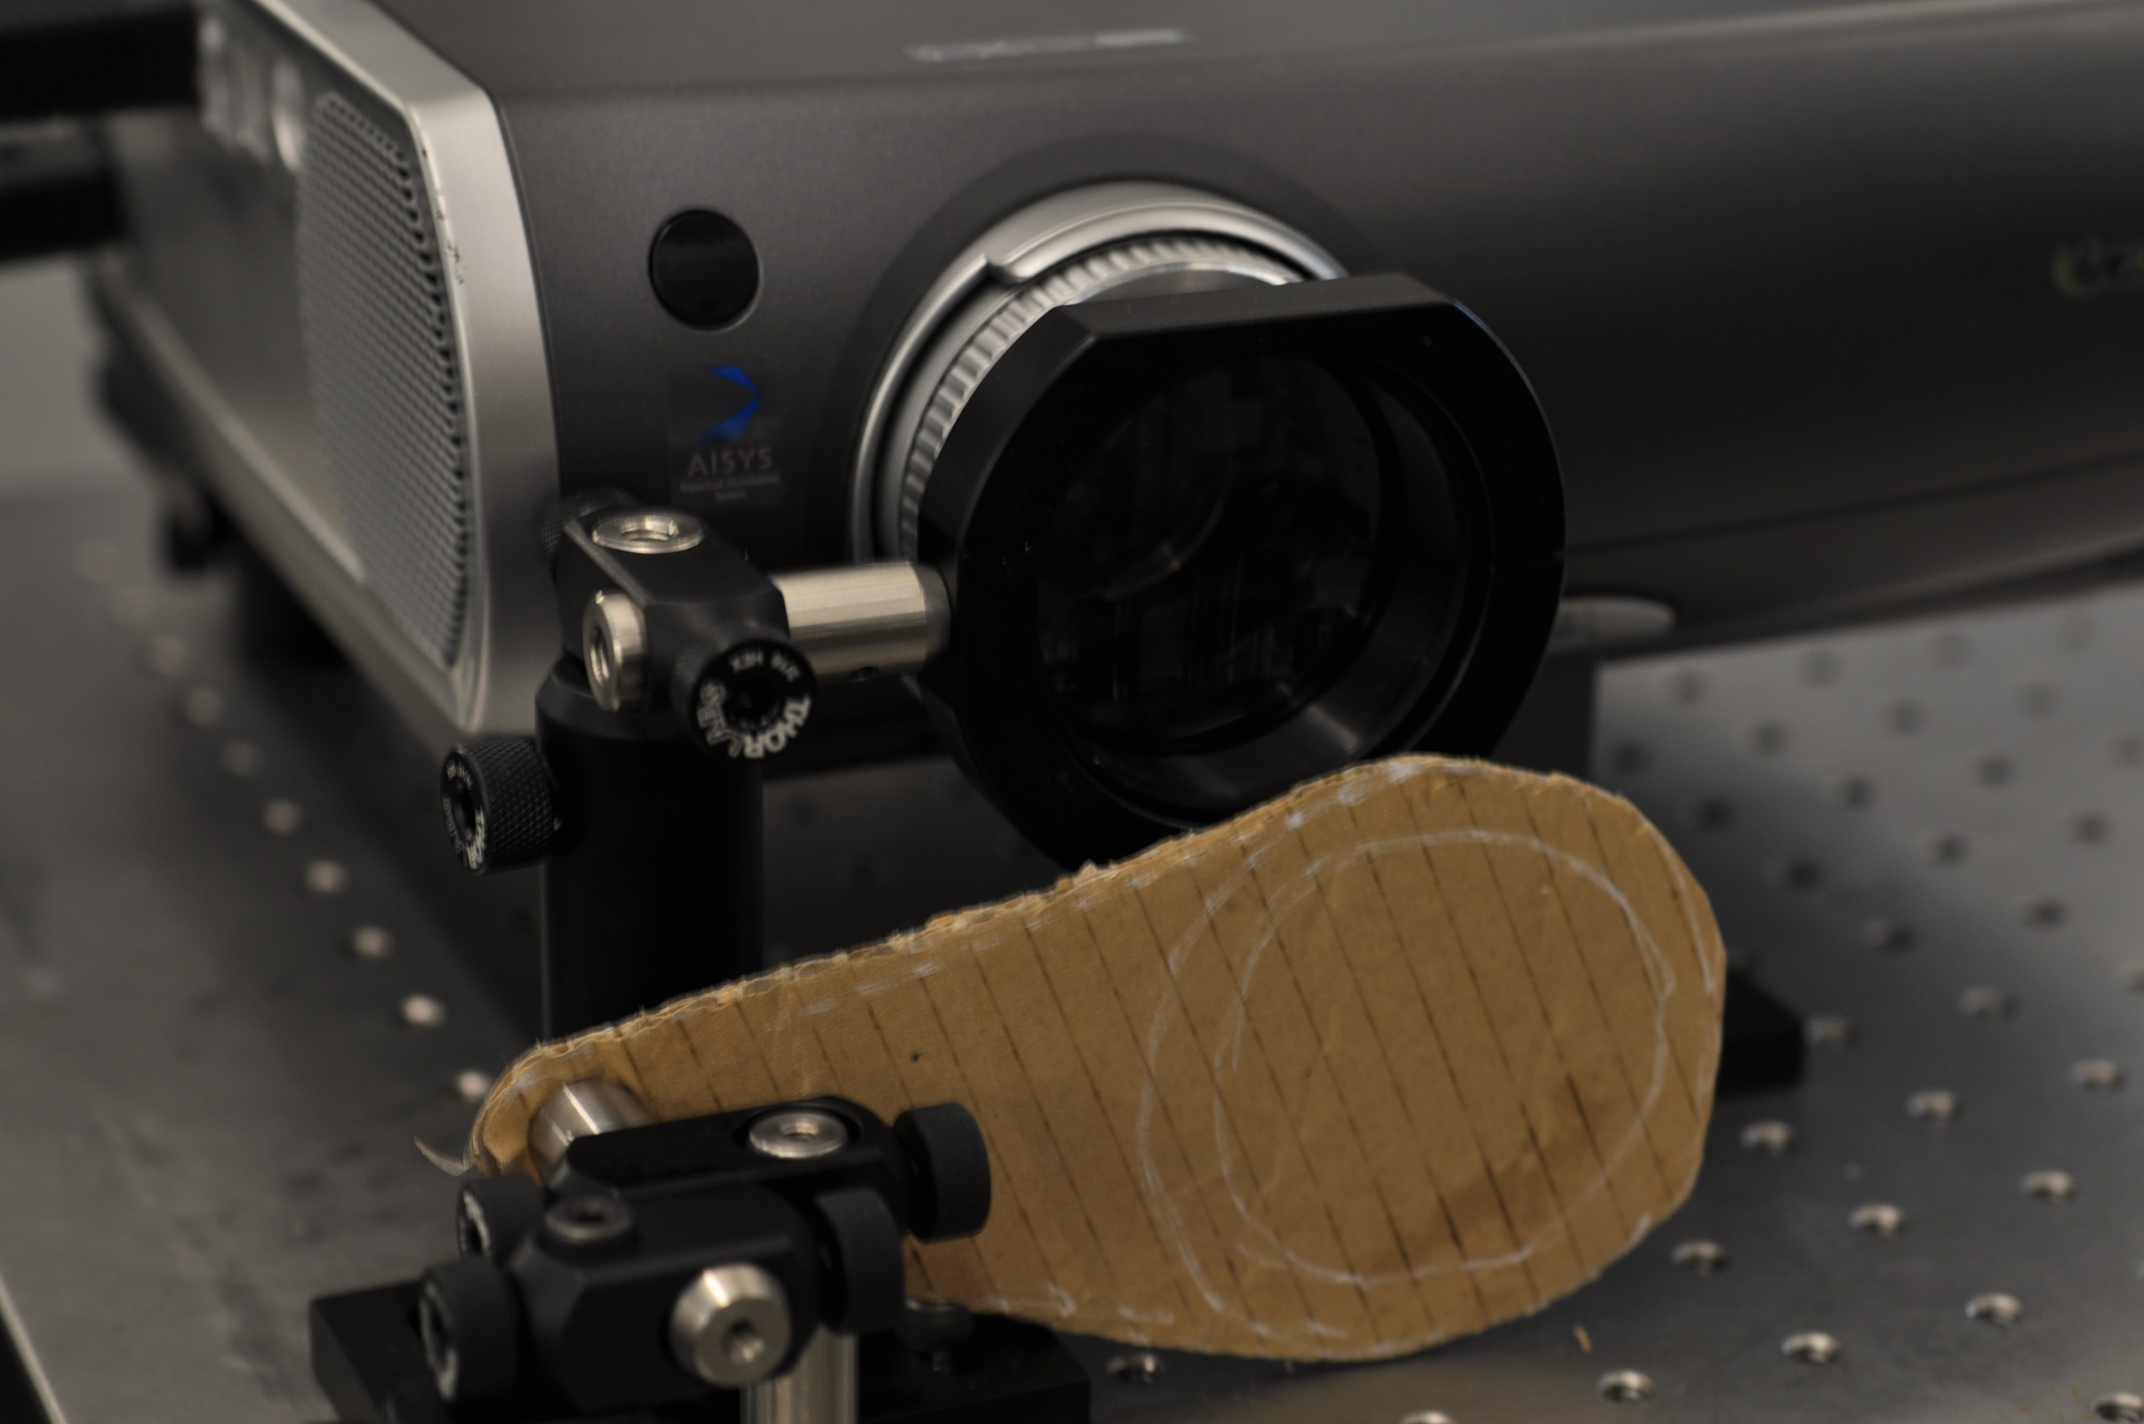
\includegraphics[width=0.3\textwidth]{pre3l.jpg}}\\
		 	\\
		  \end{tabularx}

		  \begin{tabularx}{\textwidth}{ XXX }
		   \item \textbf{Step 4} : \textbf{Put} a small piece of black paper on sample holder. \textbf{Ajust} the focal length by 
		   	rotating the ring shown in picture until the image is sharp enough.
		 	&\raisebox{-\height}{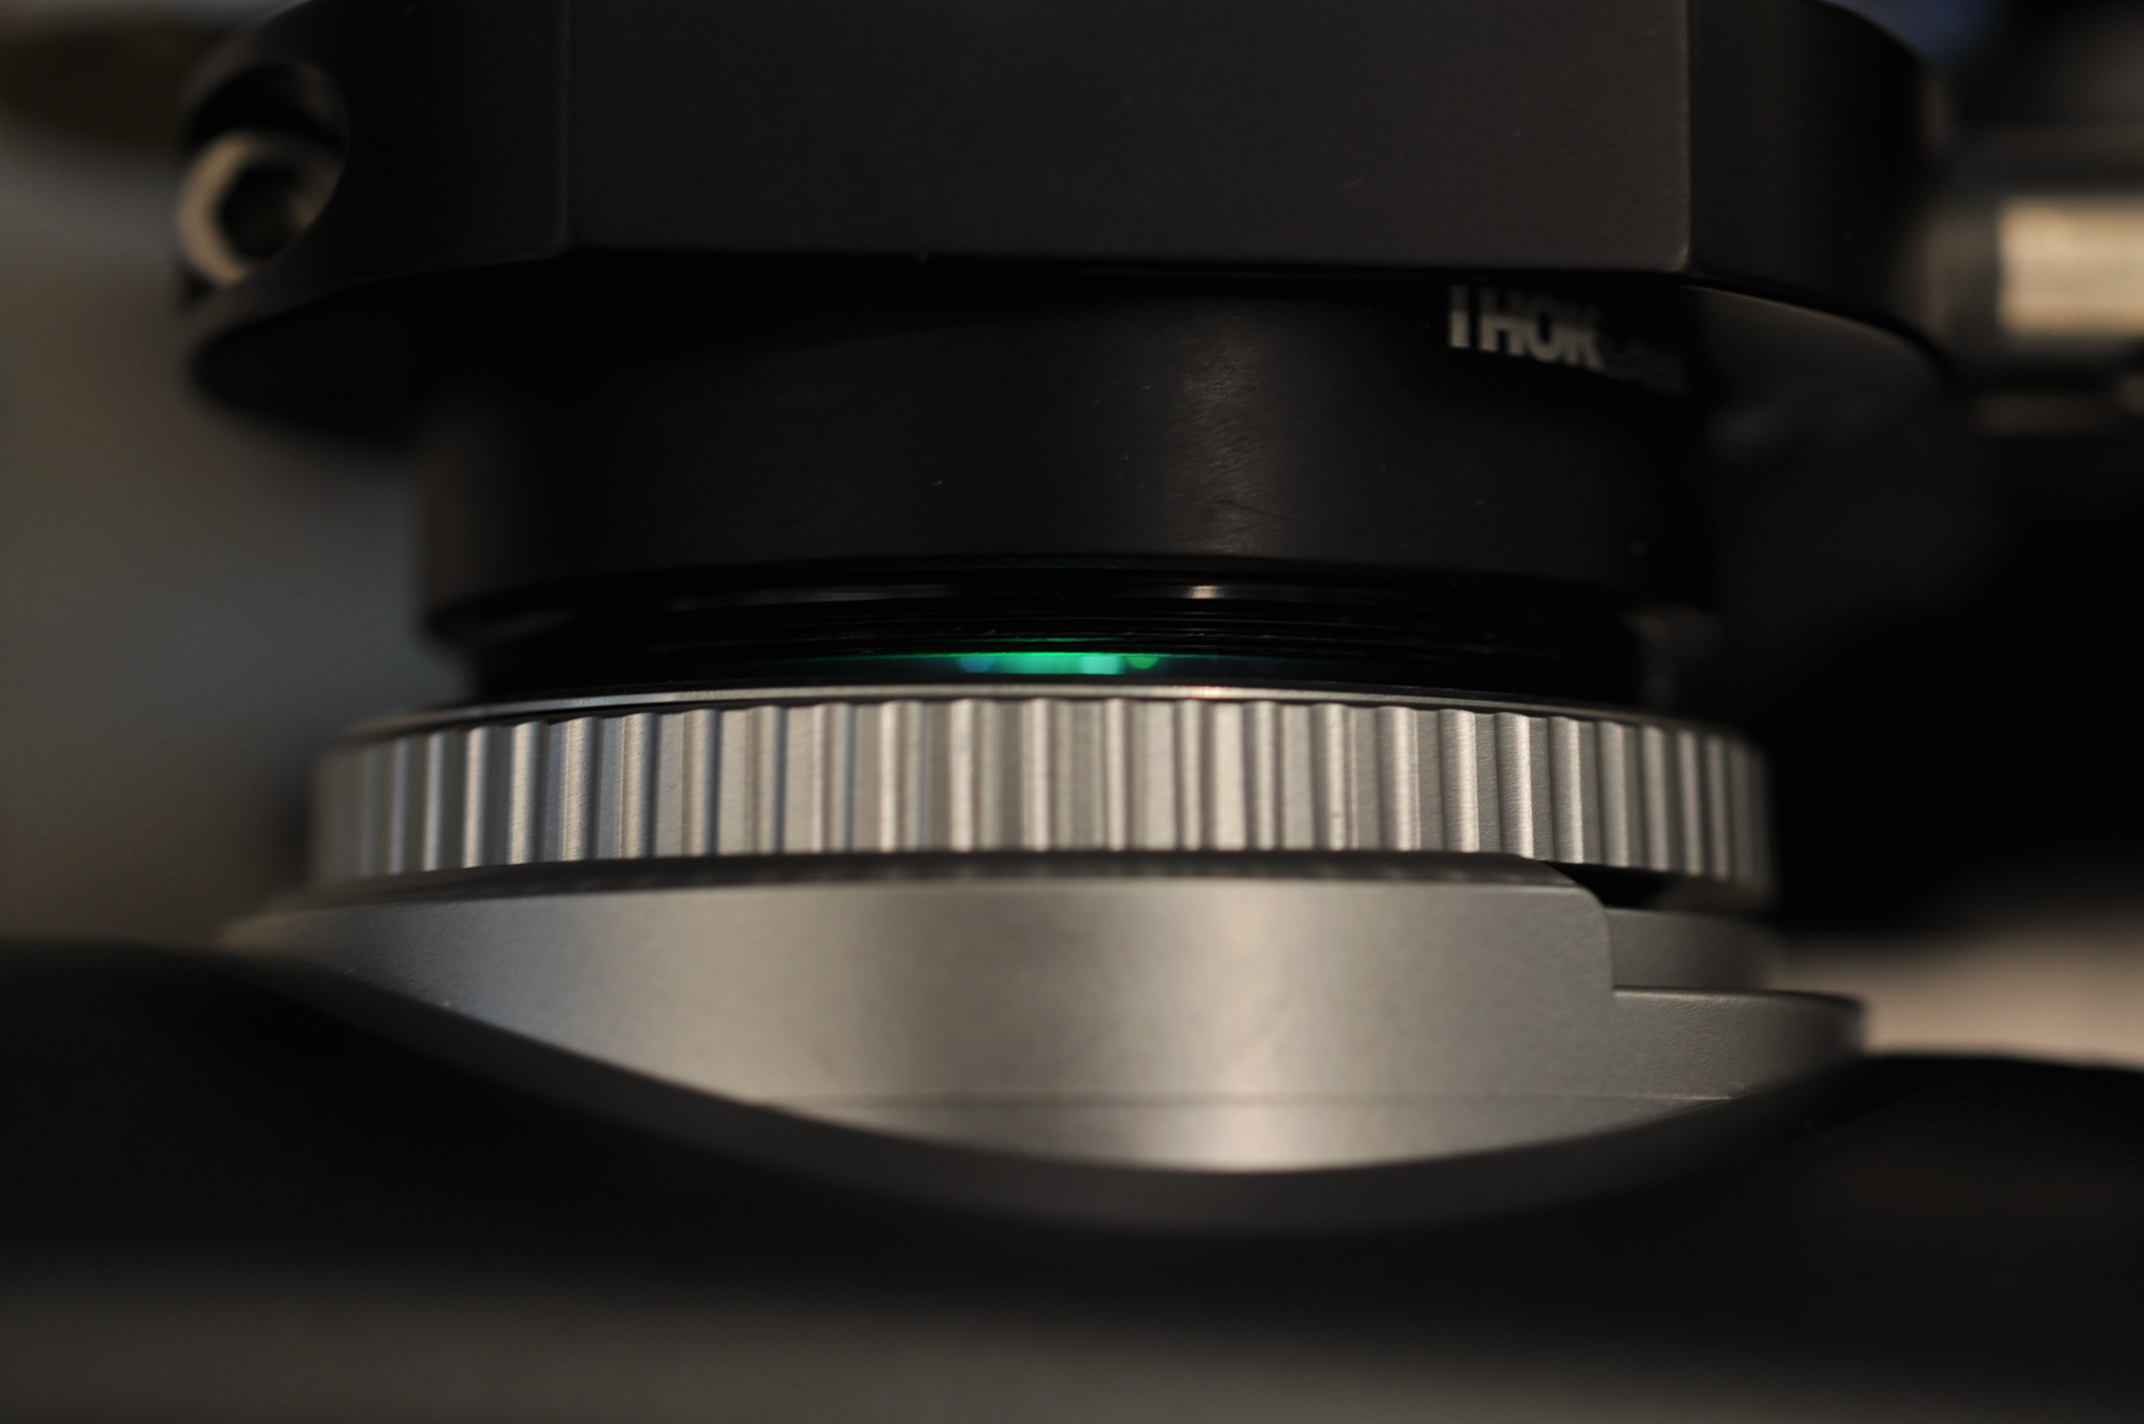
\includegraphics[width=0.3\textwidth]{pre4l.jpg}}
		 	&\raisebox{-\height}{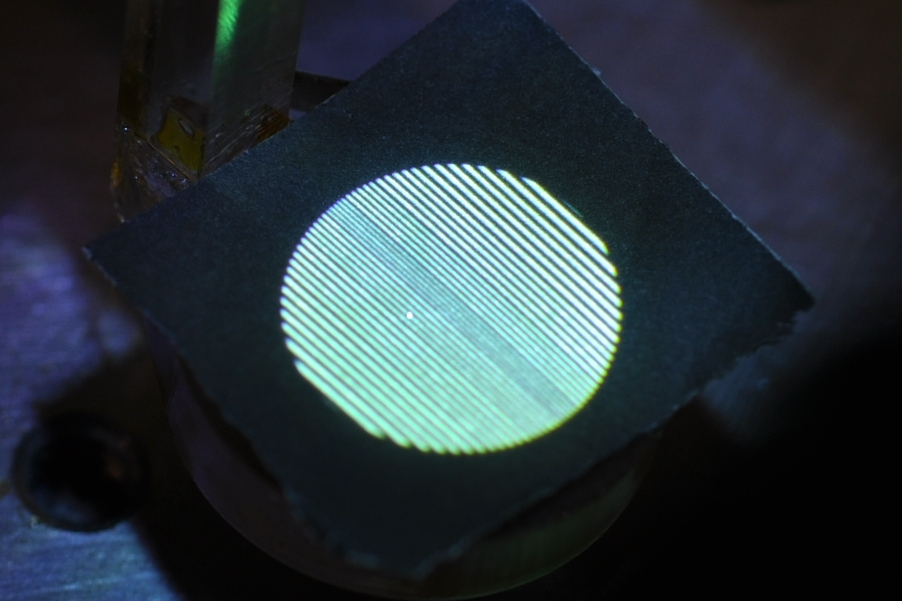
\includegraphics[width=0.3\textwidth]{pre4r.jpg}}\\
		  \end{tabularx}

		  \begin{tabularx}{\textwidth}{ XXX }
		   \item \textbf{Step 5} : \textbf{Remove} the black paper and \textbf{close} the light barrier, now the device is ready for printing.
		   \\
		  \end{tabularx}
		 \end{itemize}

		 \vspace{10pt}
		\subsection{Printing}\label{sec:printing}

		 \begin{itemize}
		  \begin{tabularx}{\textwidth}{ XXX }
		   \item \textbf{Step 1} : \textbf{Add} about 20ml of material into a beaker outside. Take away the stage assembly so that the 
		   beaker can be put on the marker. Then put the stage assembly back carefully on the marker on table.
		 	&\raisebox{-\height}{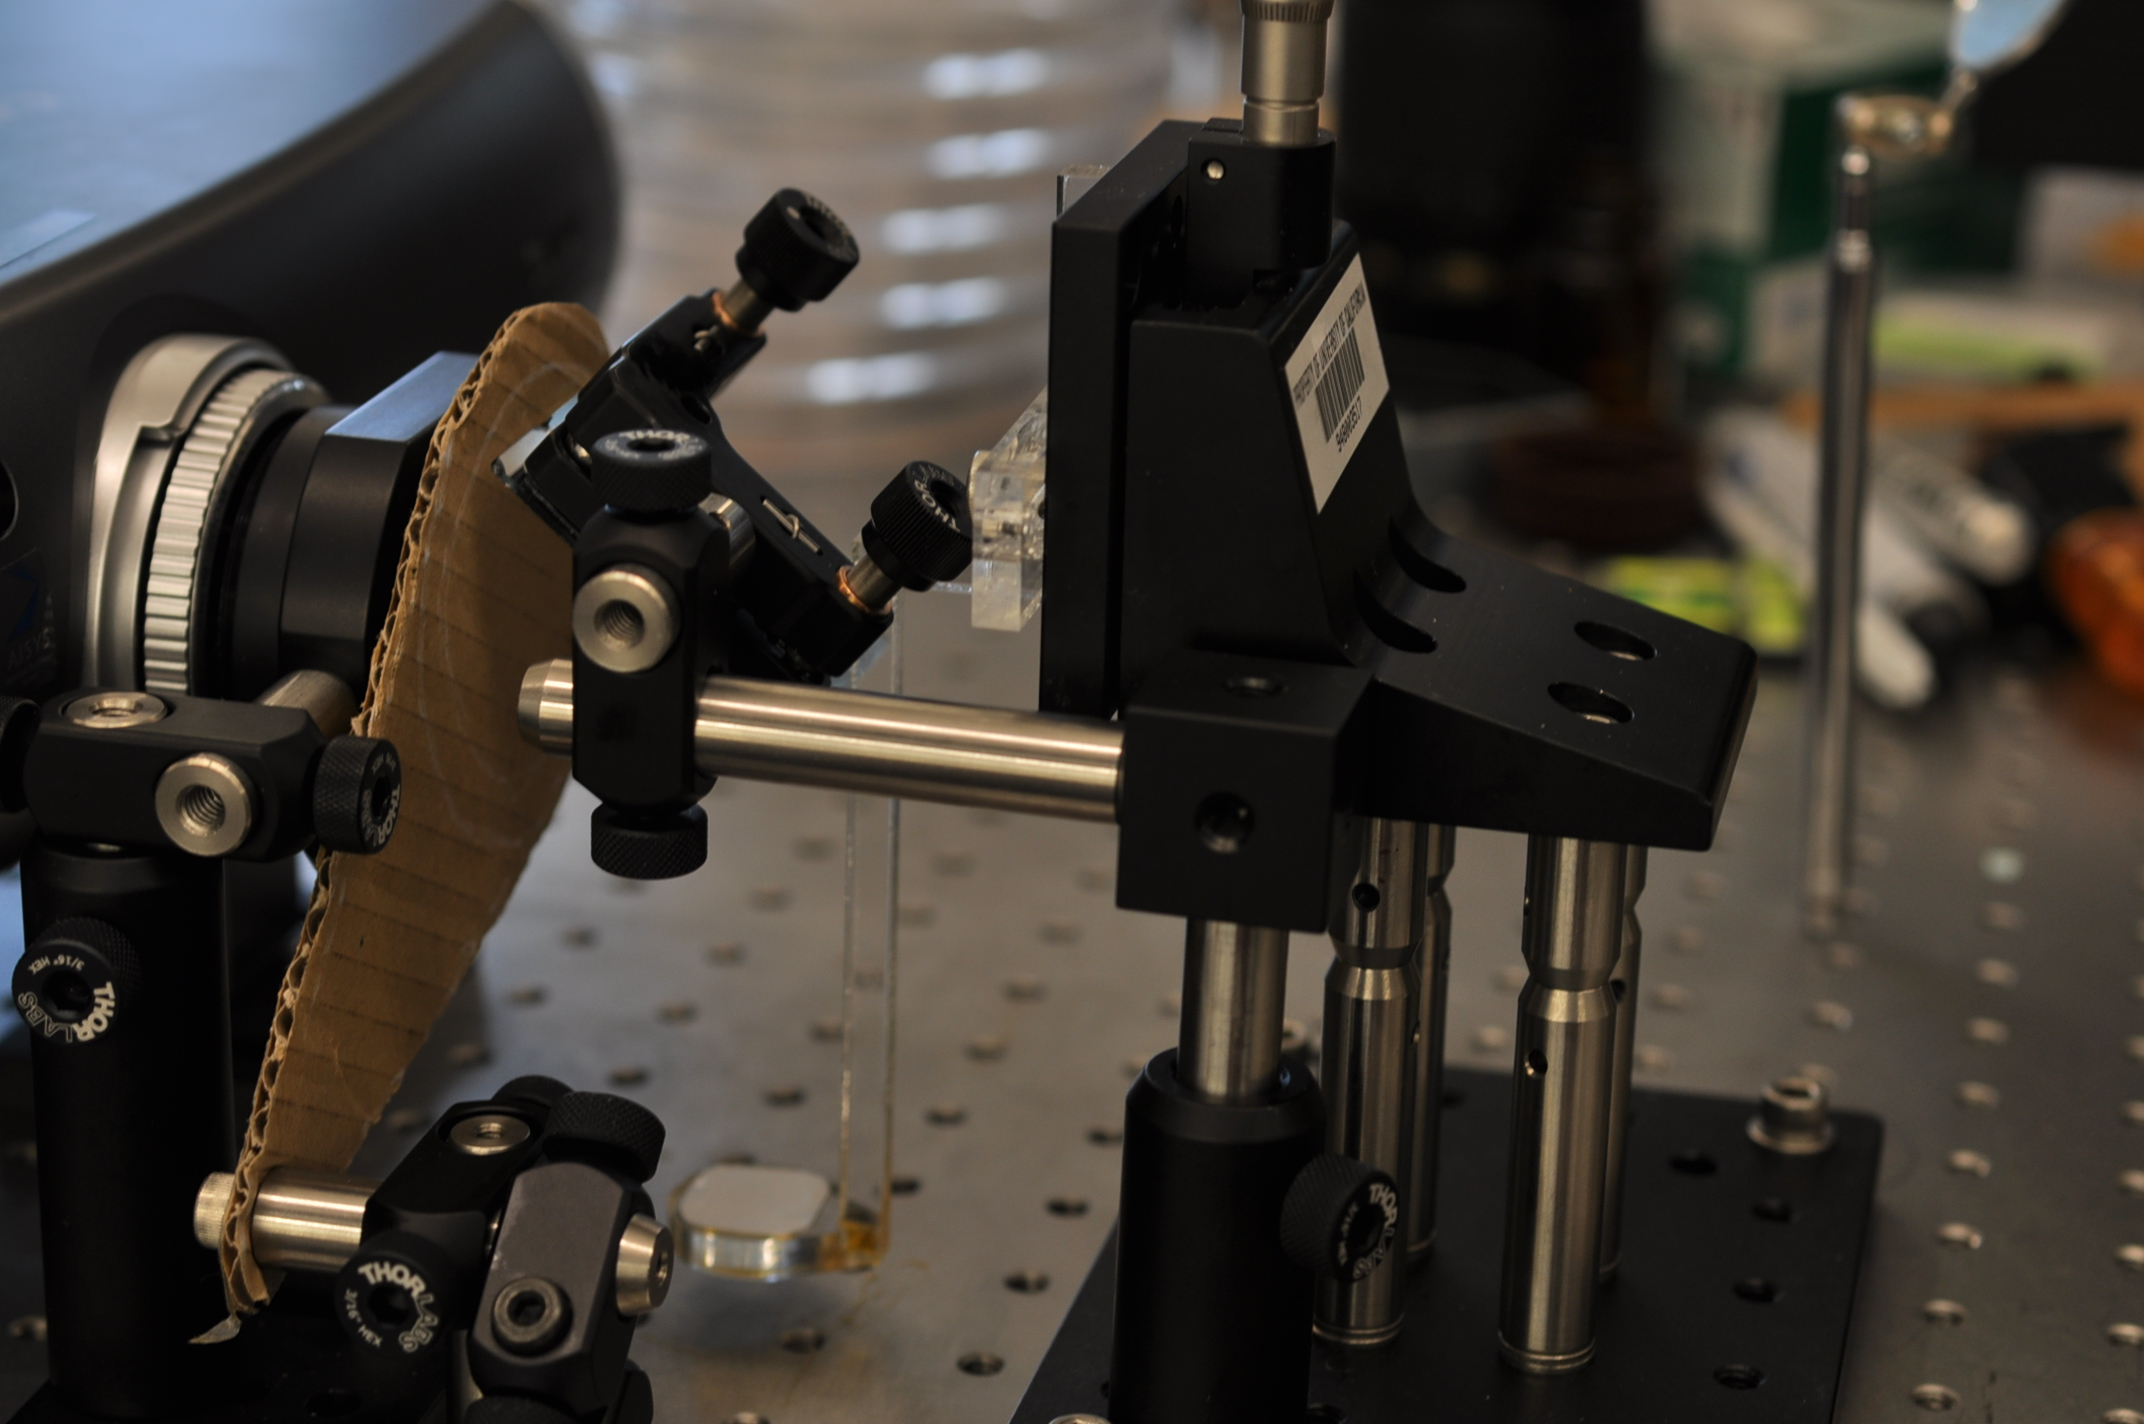
\includegraphics[width=0.3\textwidth]{pre5l.jpg}}
		 	&\raisebox{-\height}{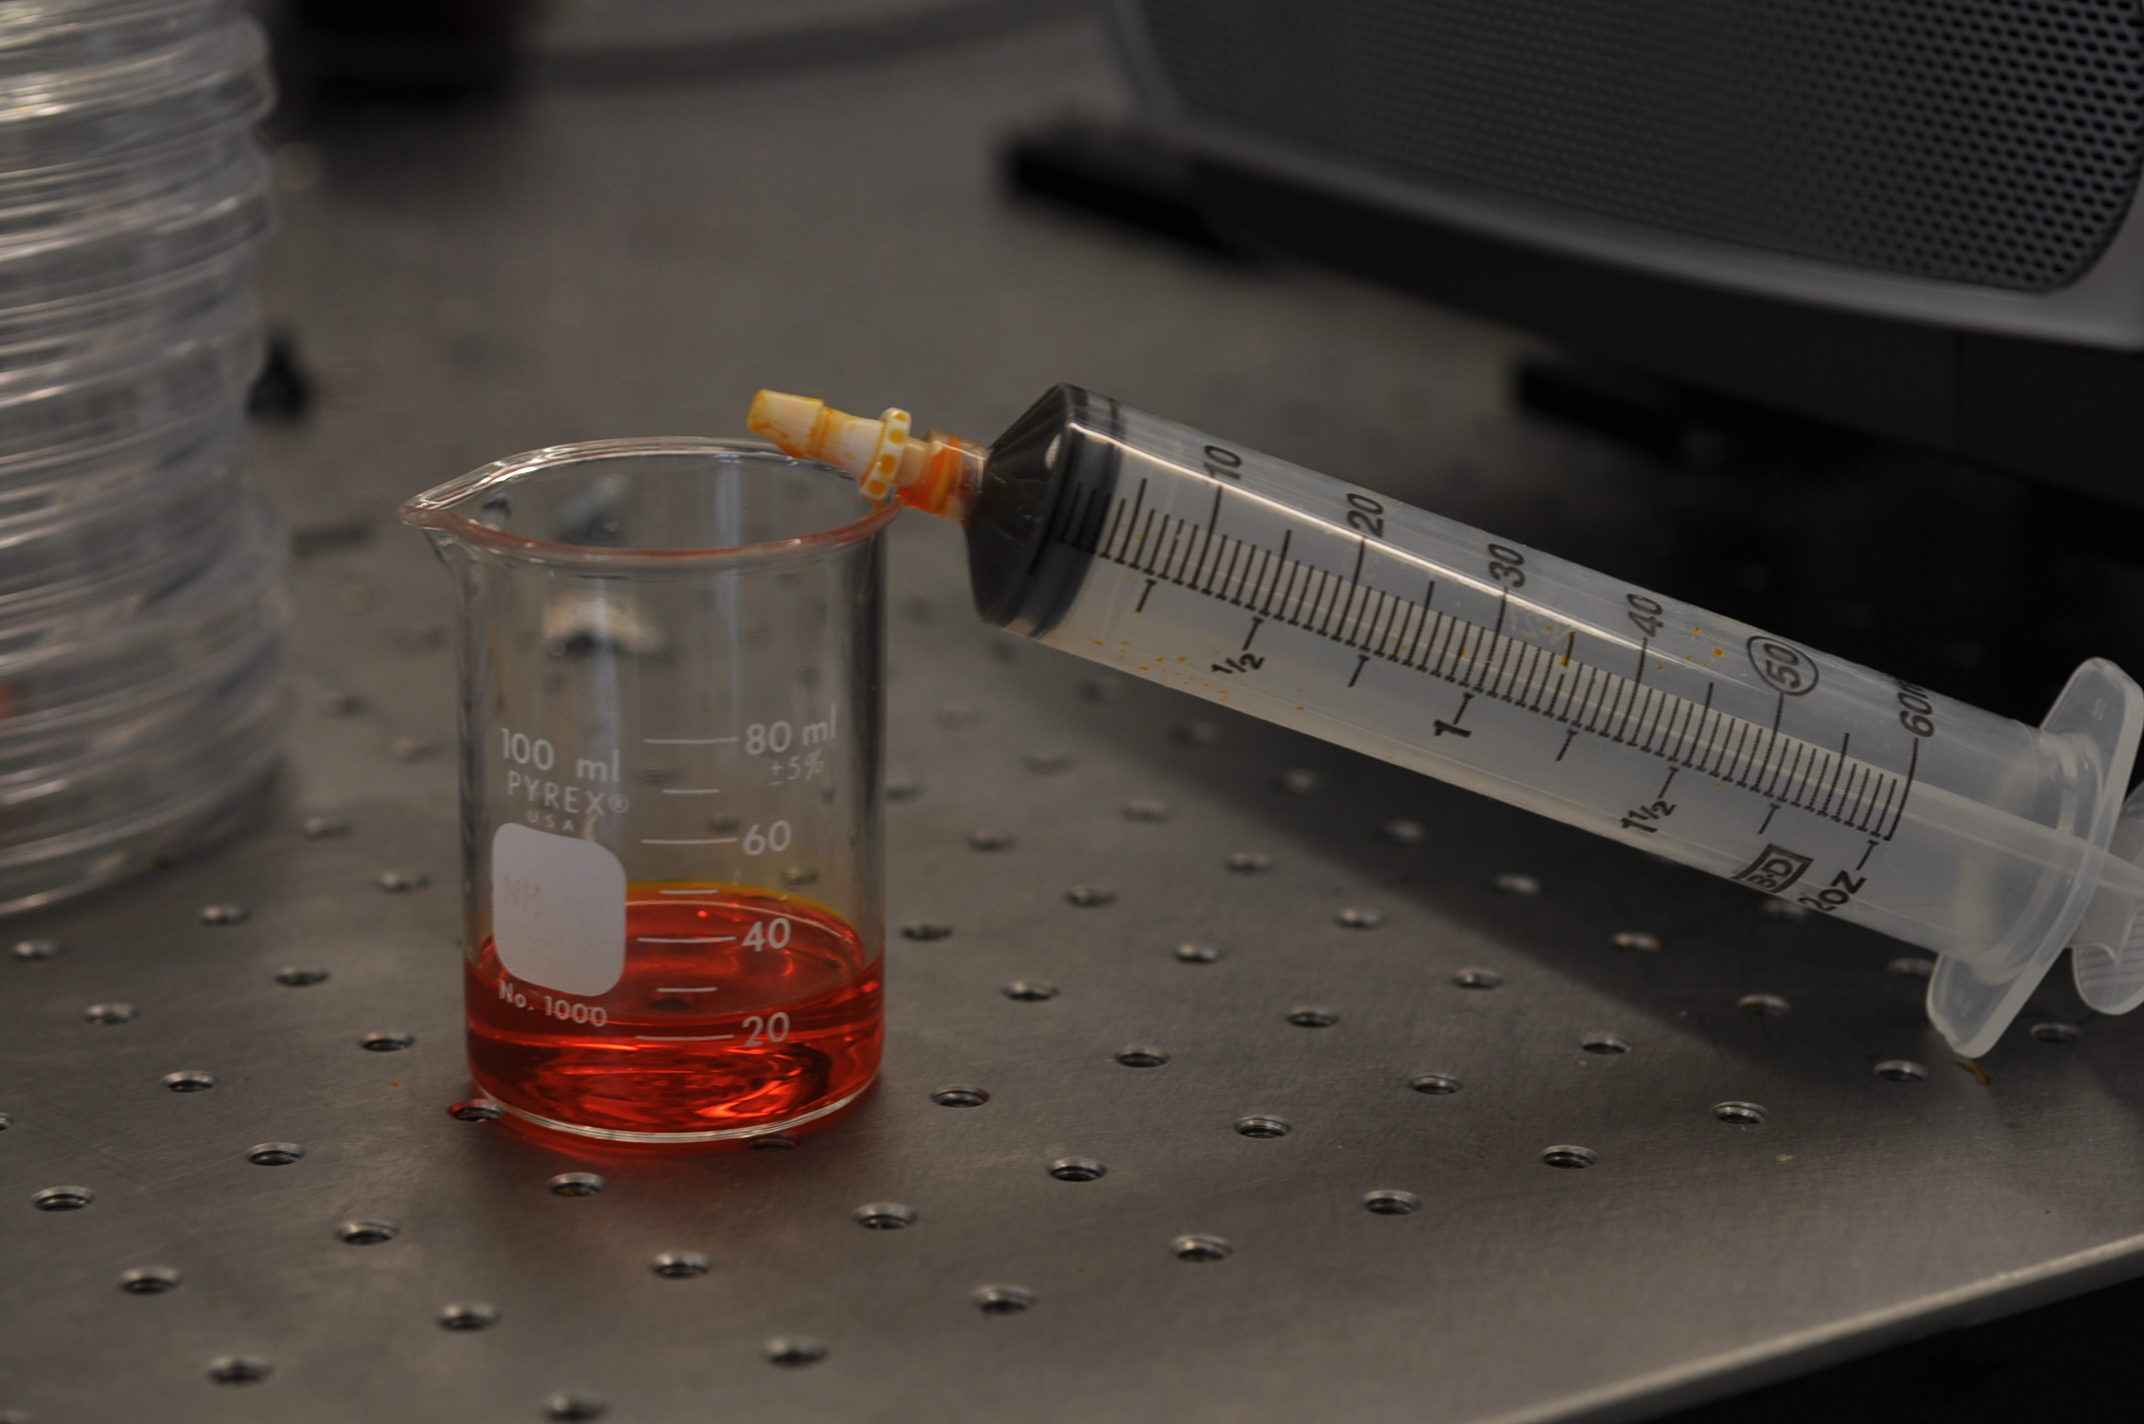
\includegraphics[width=0.3\textwidth]{pre5r.jpg}}\\
		 	\\
		  \end{tabularx}

		  \begin{tabularx}{\textwidth}{ XXX }
		   \item \textbf{Step 2} : \textbf{Add} material carefully with a small syringe. When the liquid level is just above the 
		 	printing panel, it's ready to print.
		 	&\raisebox{-\height}{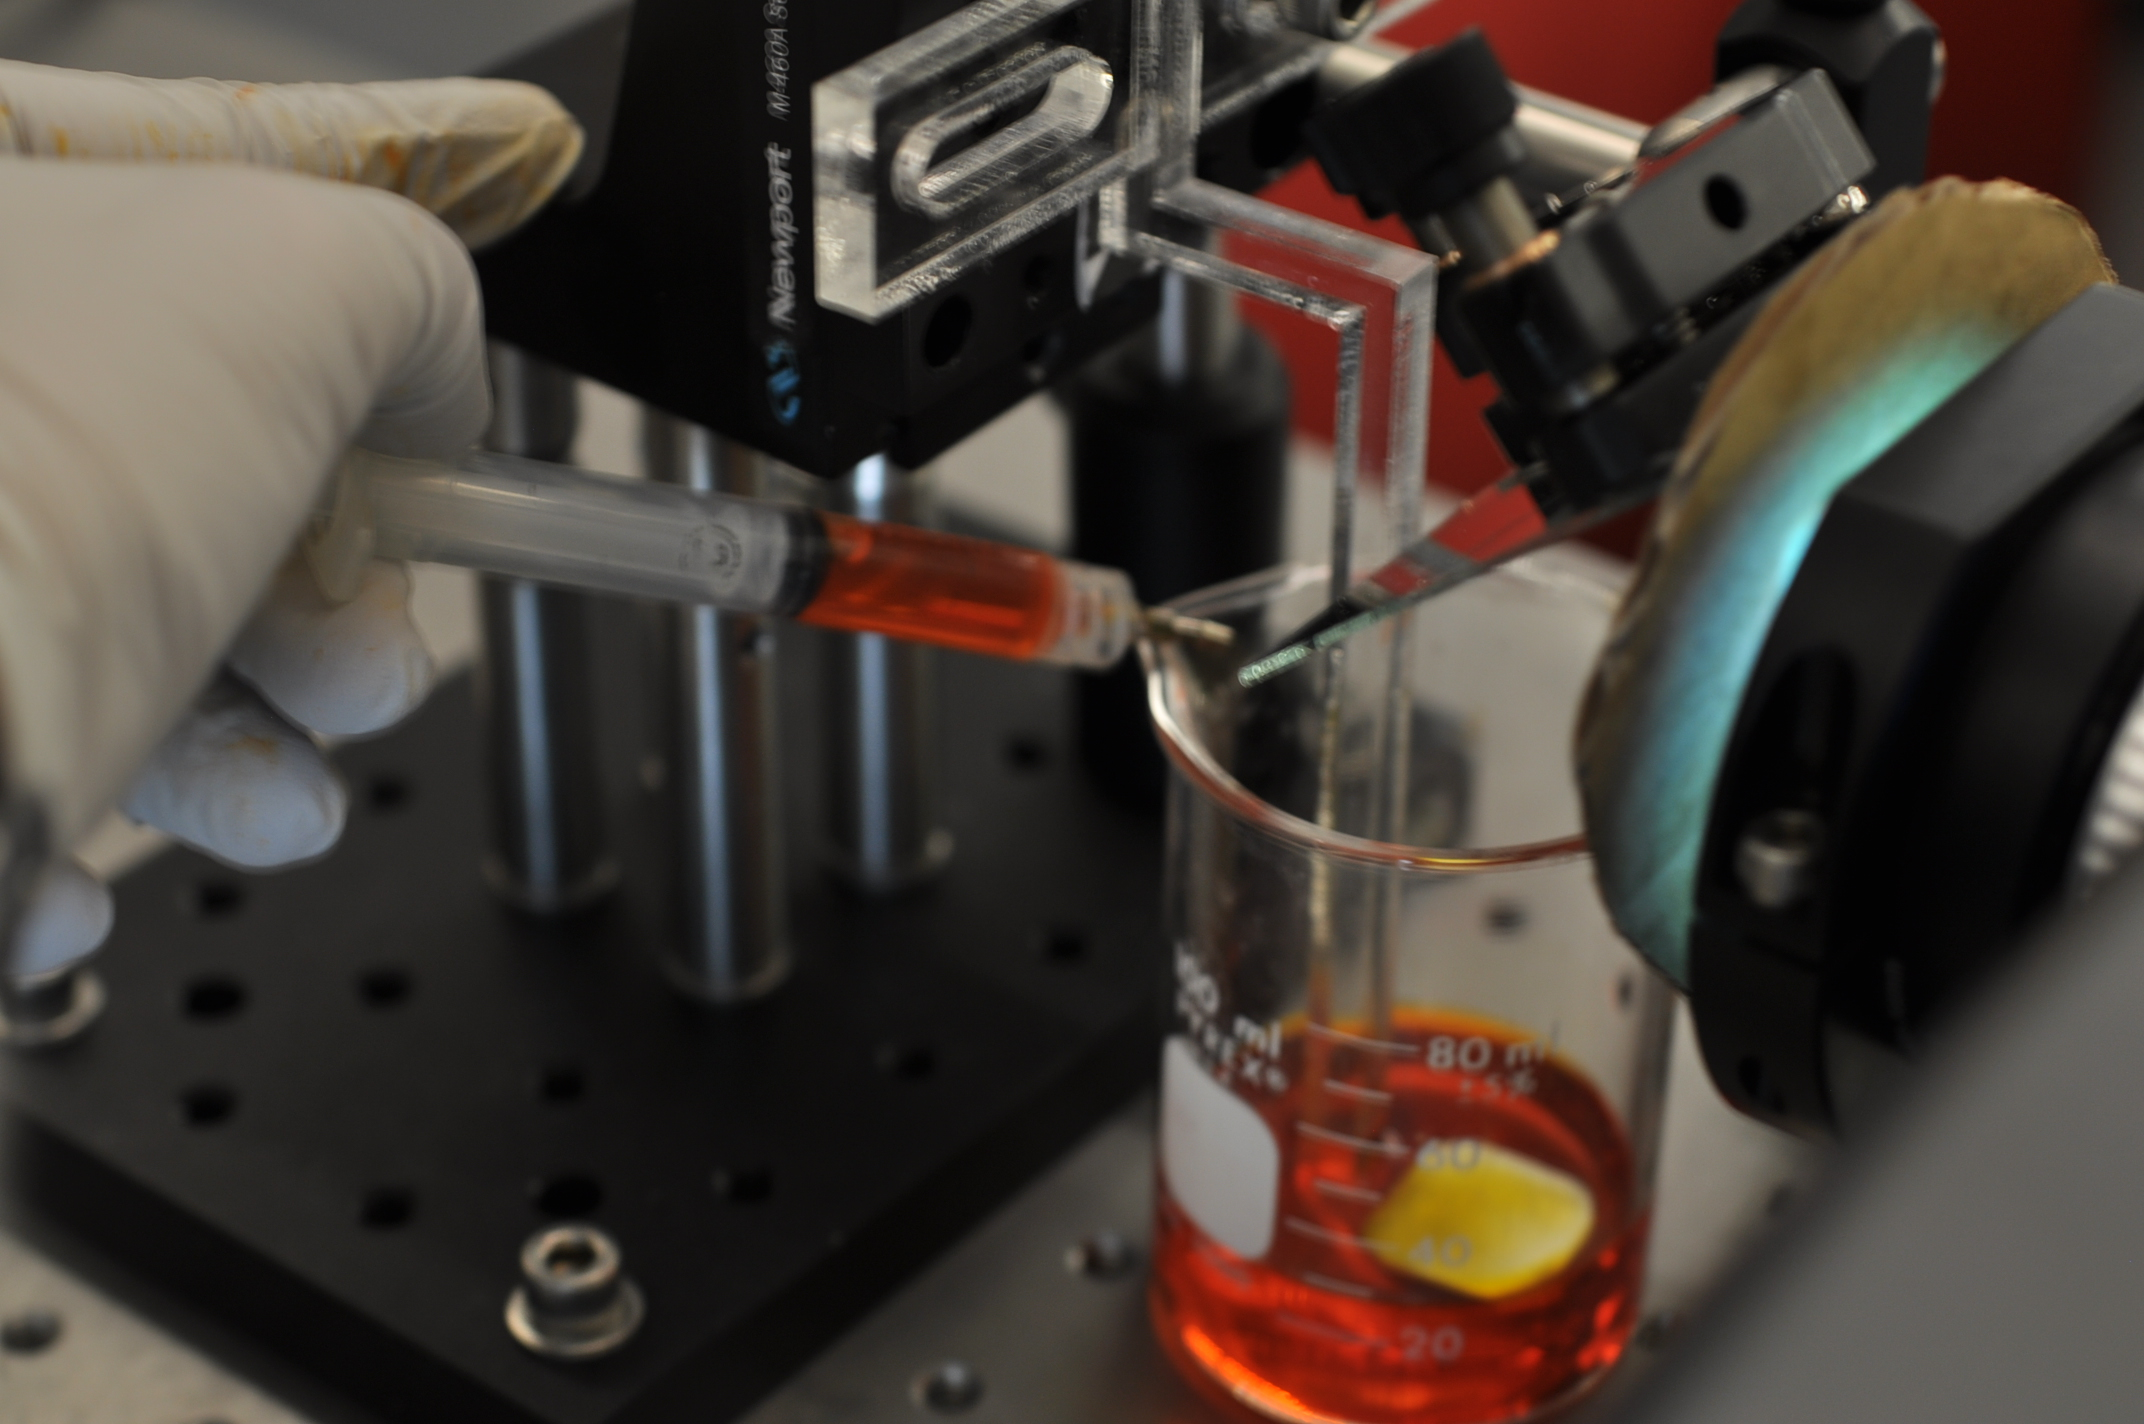
\includegraphics[width=0.3\textwidth]{pre6l.jpg}}
		 	&\raisebox{-\height}{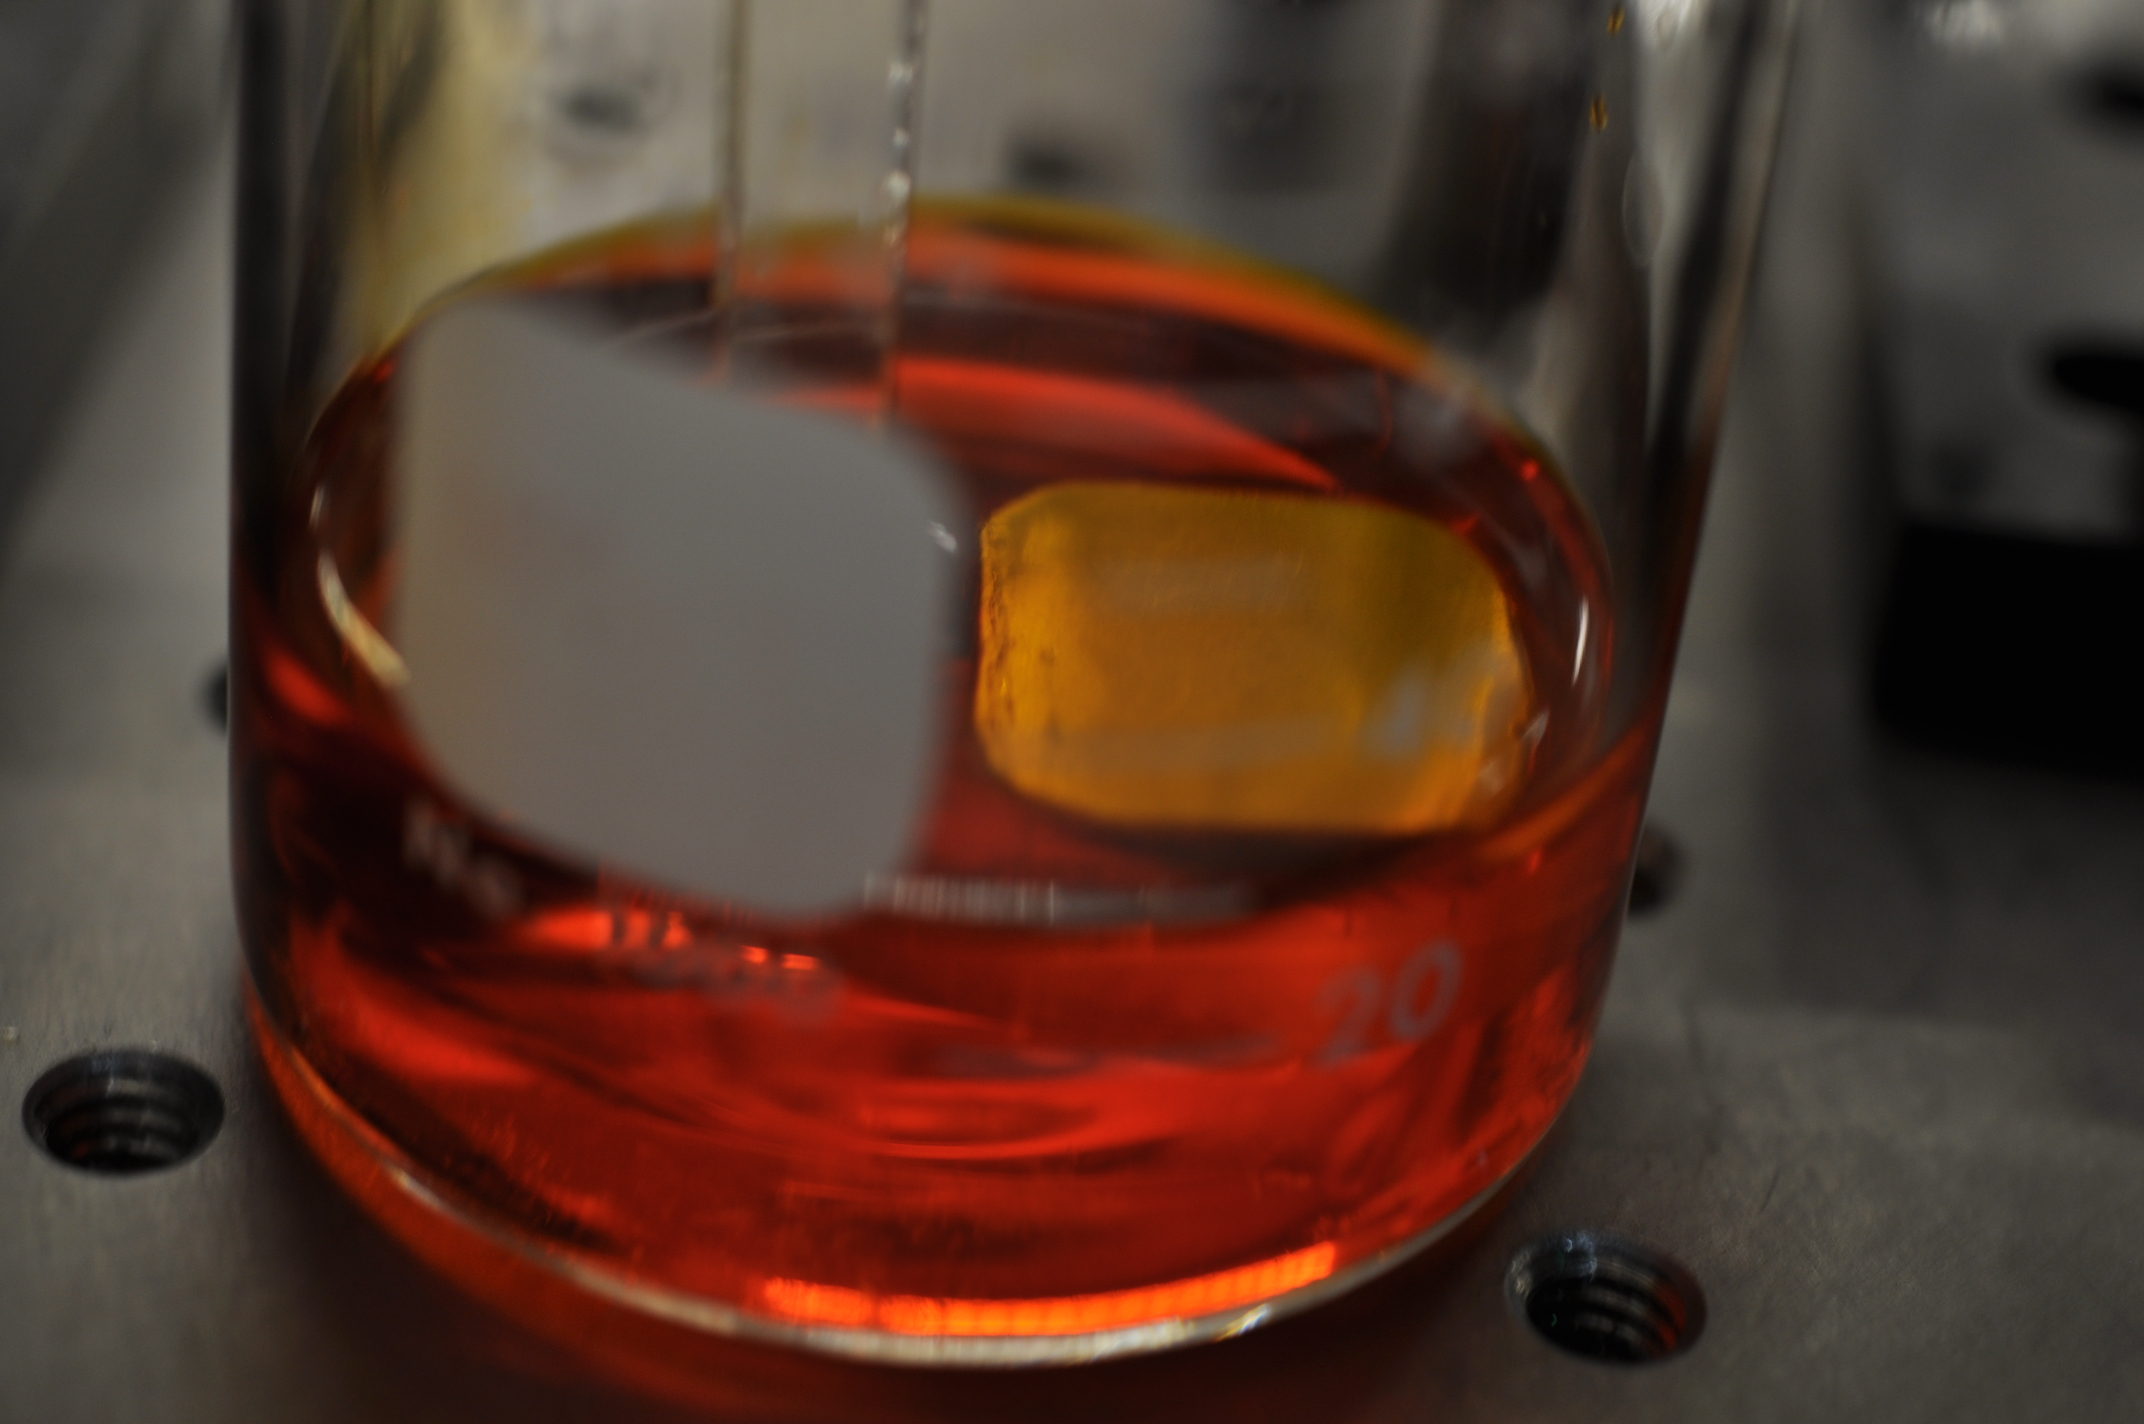
\includegraphics[width=0.3\textwidth]{pre6r.jpg}}\\
		 	\\
		  \end{tabularx}

		  \begin{tabularx}{\textwidth}{ XXX }
		 	\item \textbf{Step 3} : \textbf{Set} the image you need to print as desktop background. \textbf{Open} 'voice.py' and input the 
		 	parameters. Then Go back to the printer immediately. See more in Sec1.2.
		 	&\raisebox{-0.9\height}{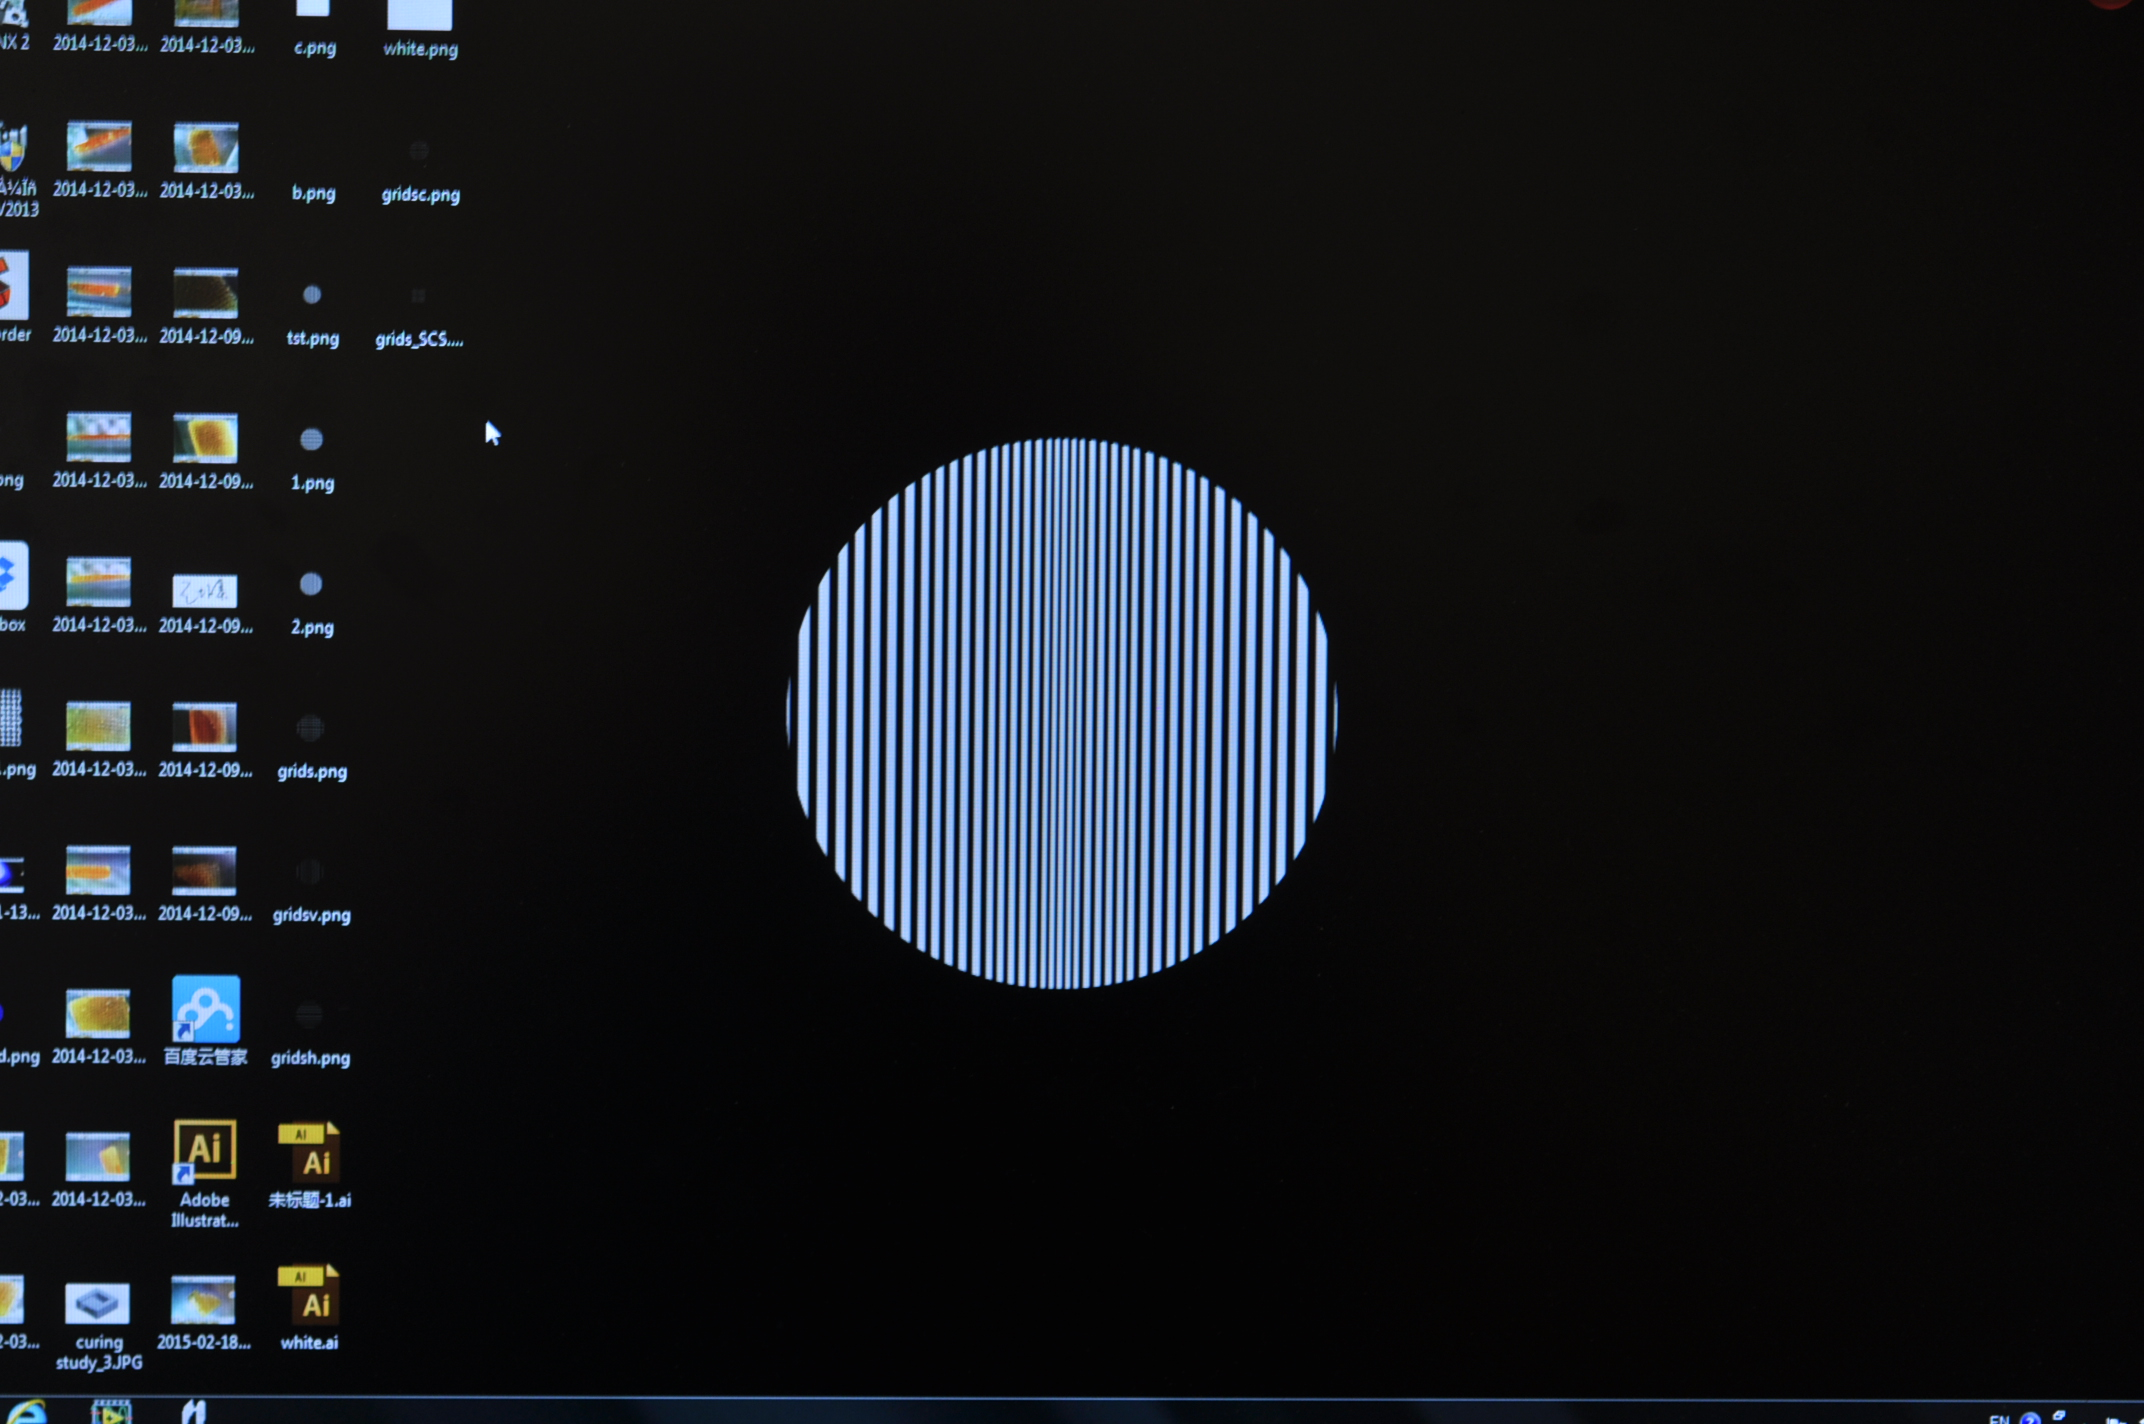
\includegraphics[width=0.3\textwidth]{prt1l.jpg}}
		 	&\raisebox{-0.9\height}{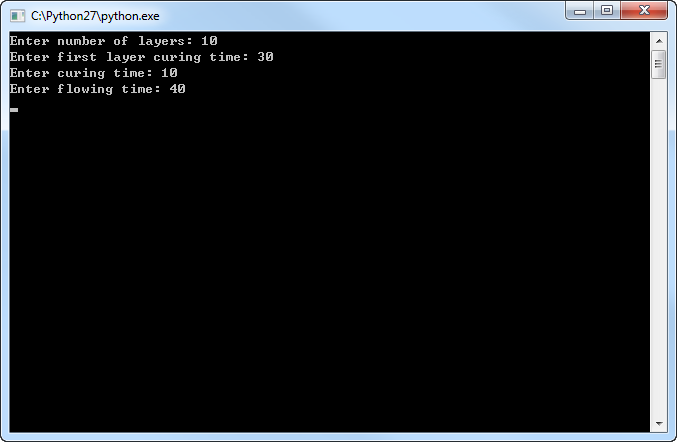
\includegraphics[width=0.3\textwidth]{prt1r.png}}\\
		 	\\
		 	\end{tabularx}

		  \begin{tabularx}{\textwidth}{ XXX }
		 	\item \textbf{Step 4} : Follow the voice instruction. When hearing 'Projecting', \textbf{open} the light barrier. 
		 	After several seconds set in step 1, you will hear 'finish' which means you should \textbf{close} the barrier.
		 	&\raisebox{-\height}{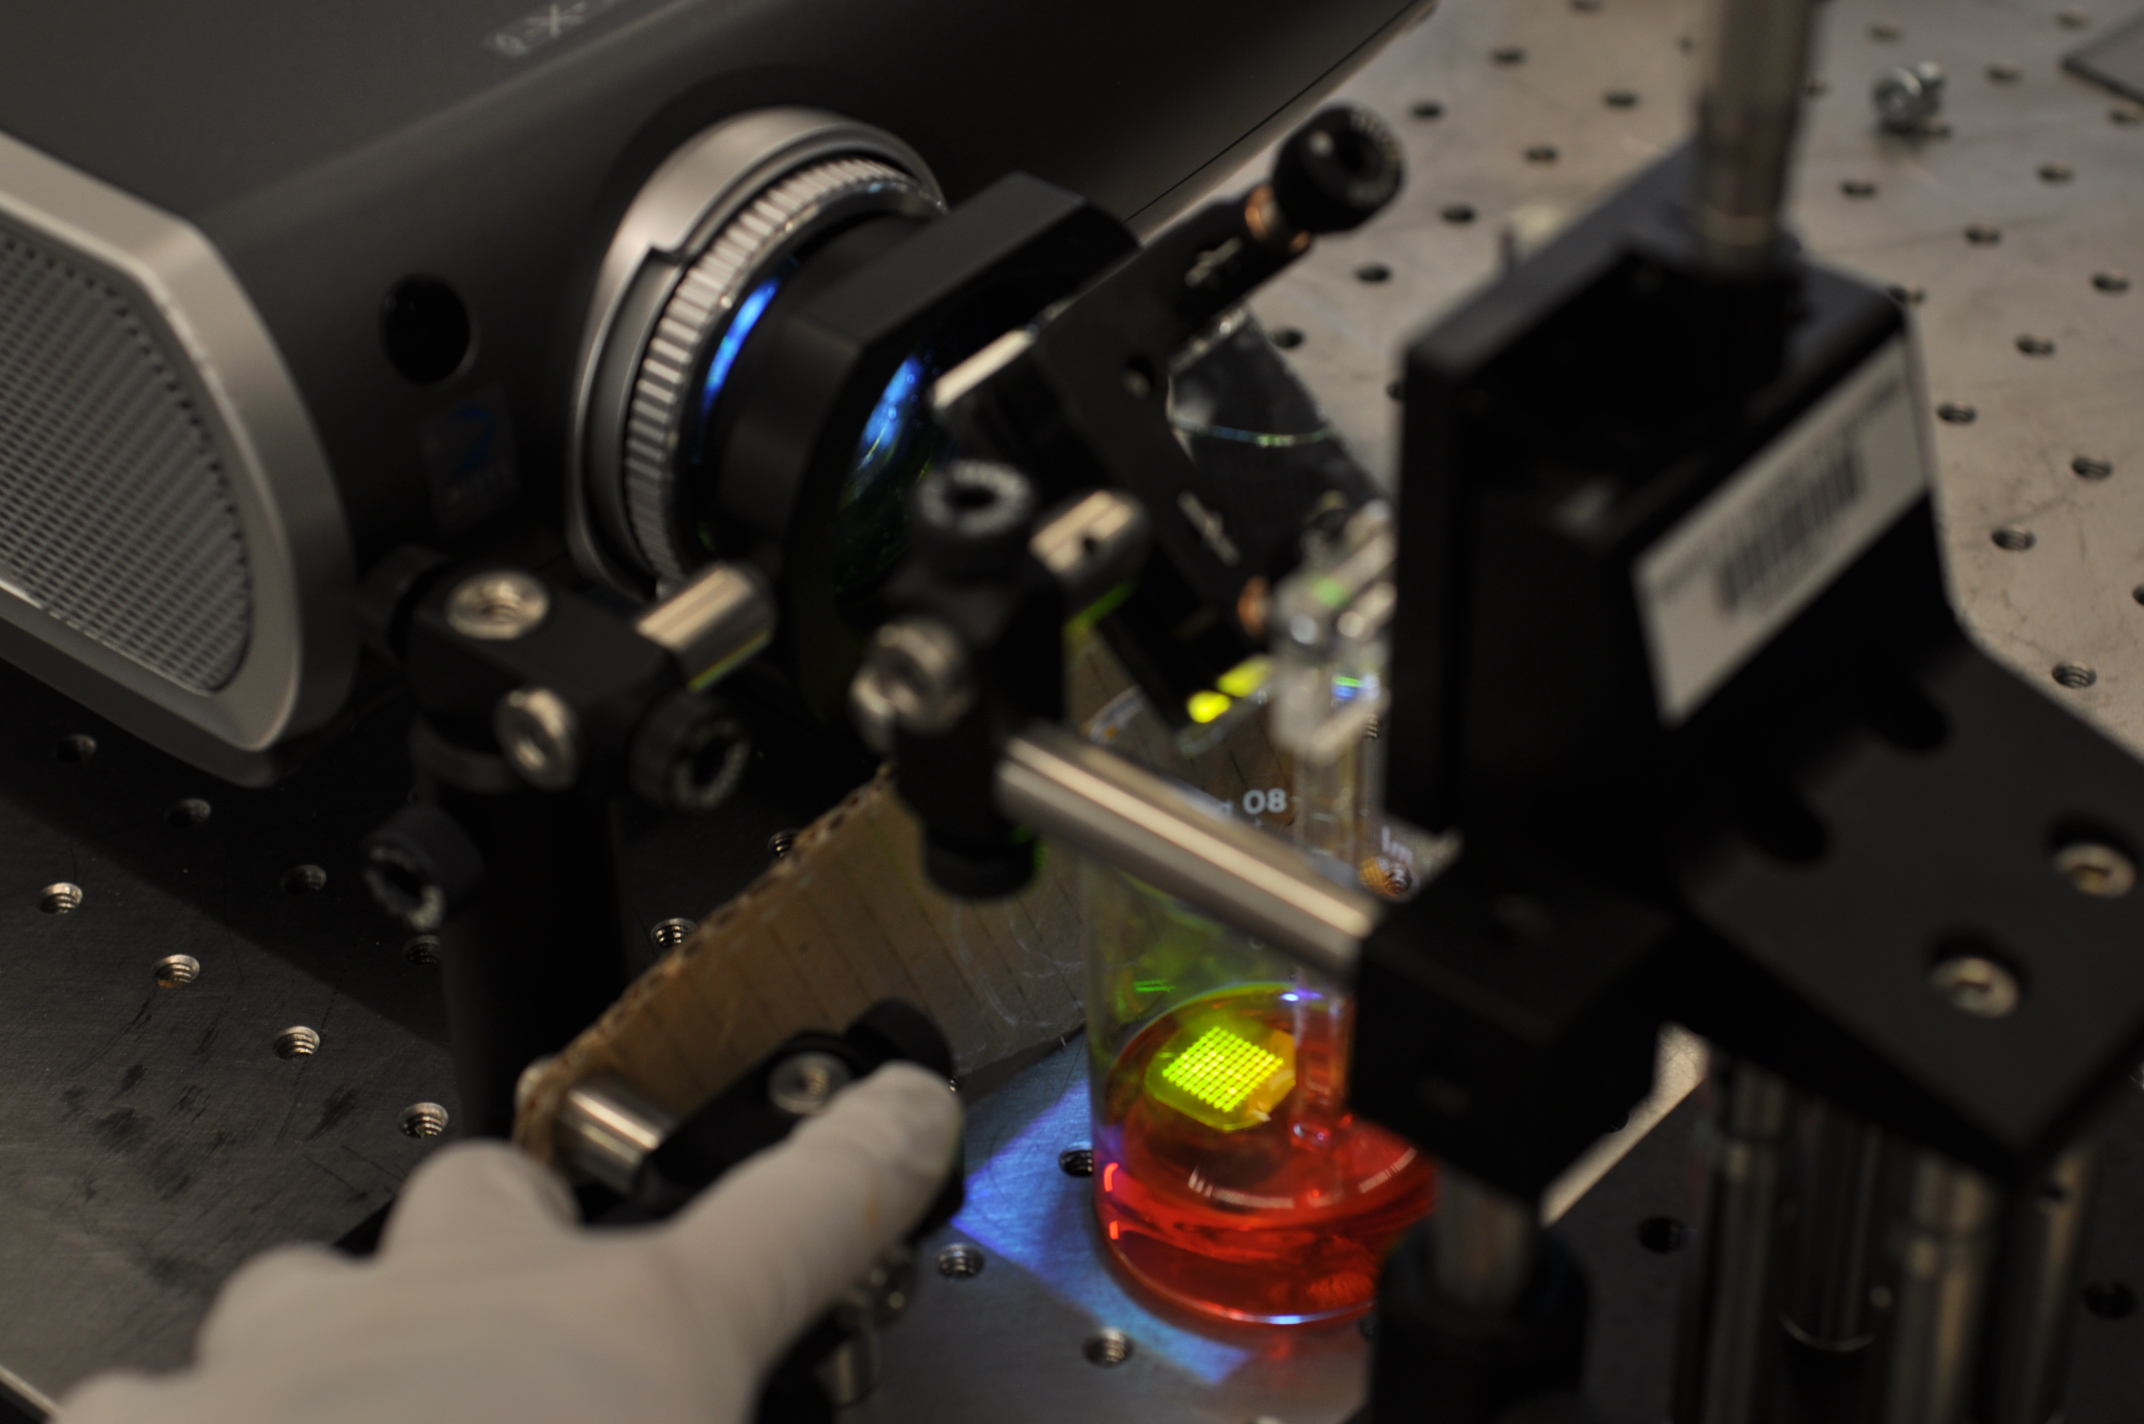
\includegraphics[width=0.3\textwidth]{prt2l.jpg}}
		 	&\raisebox{-\height}{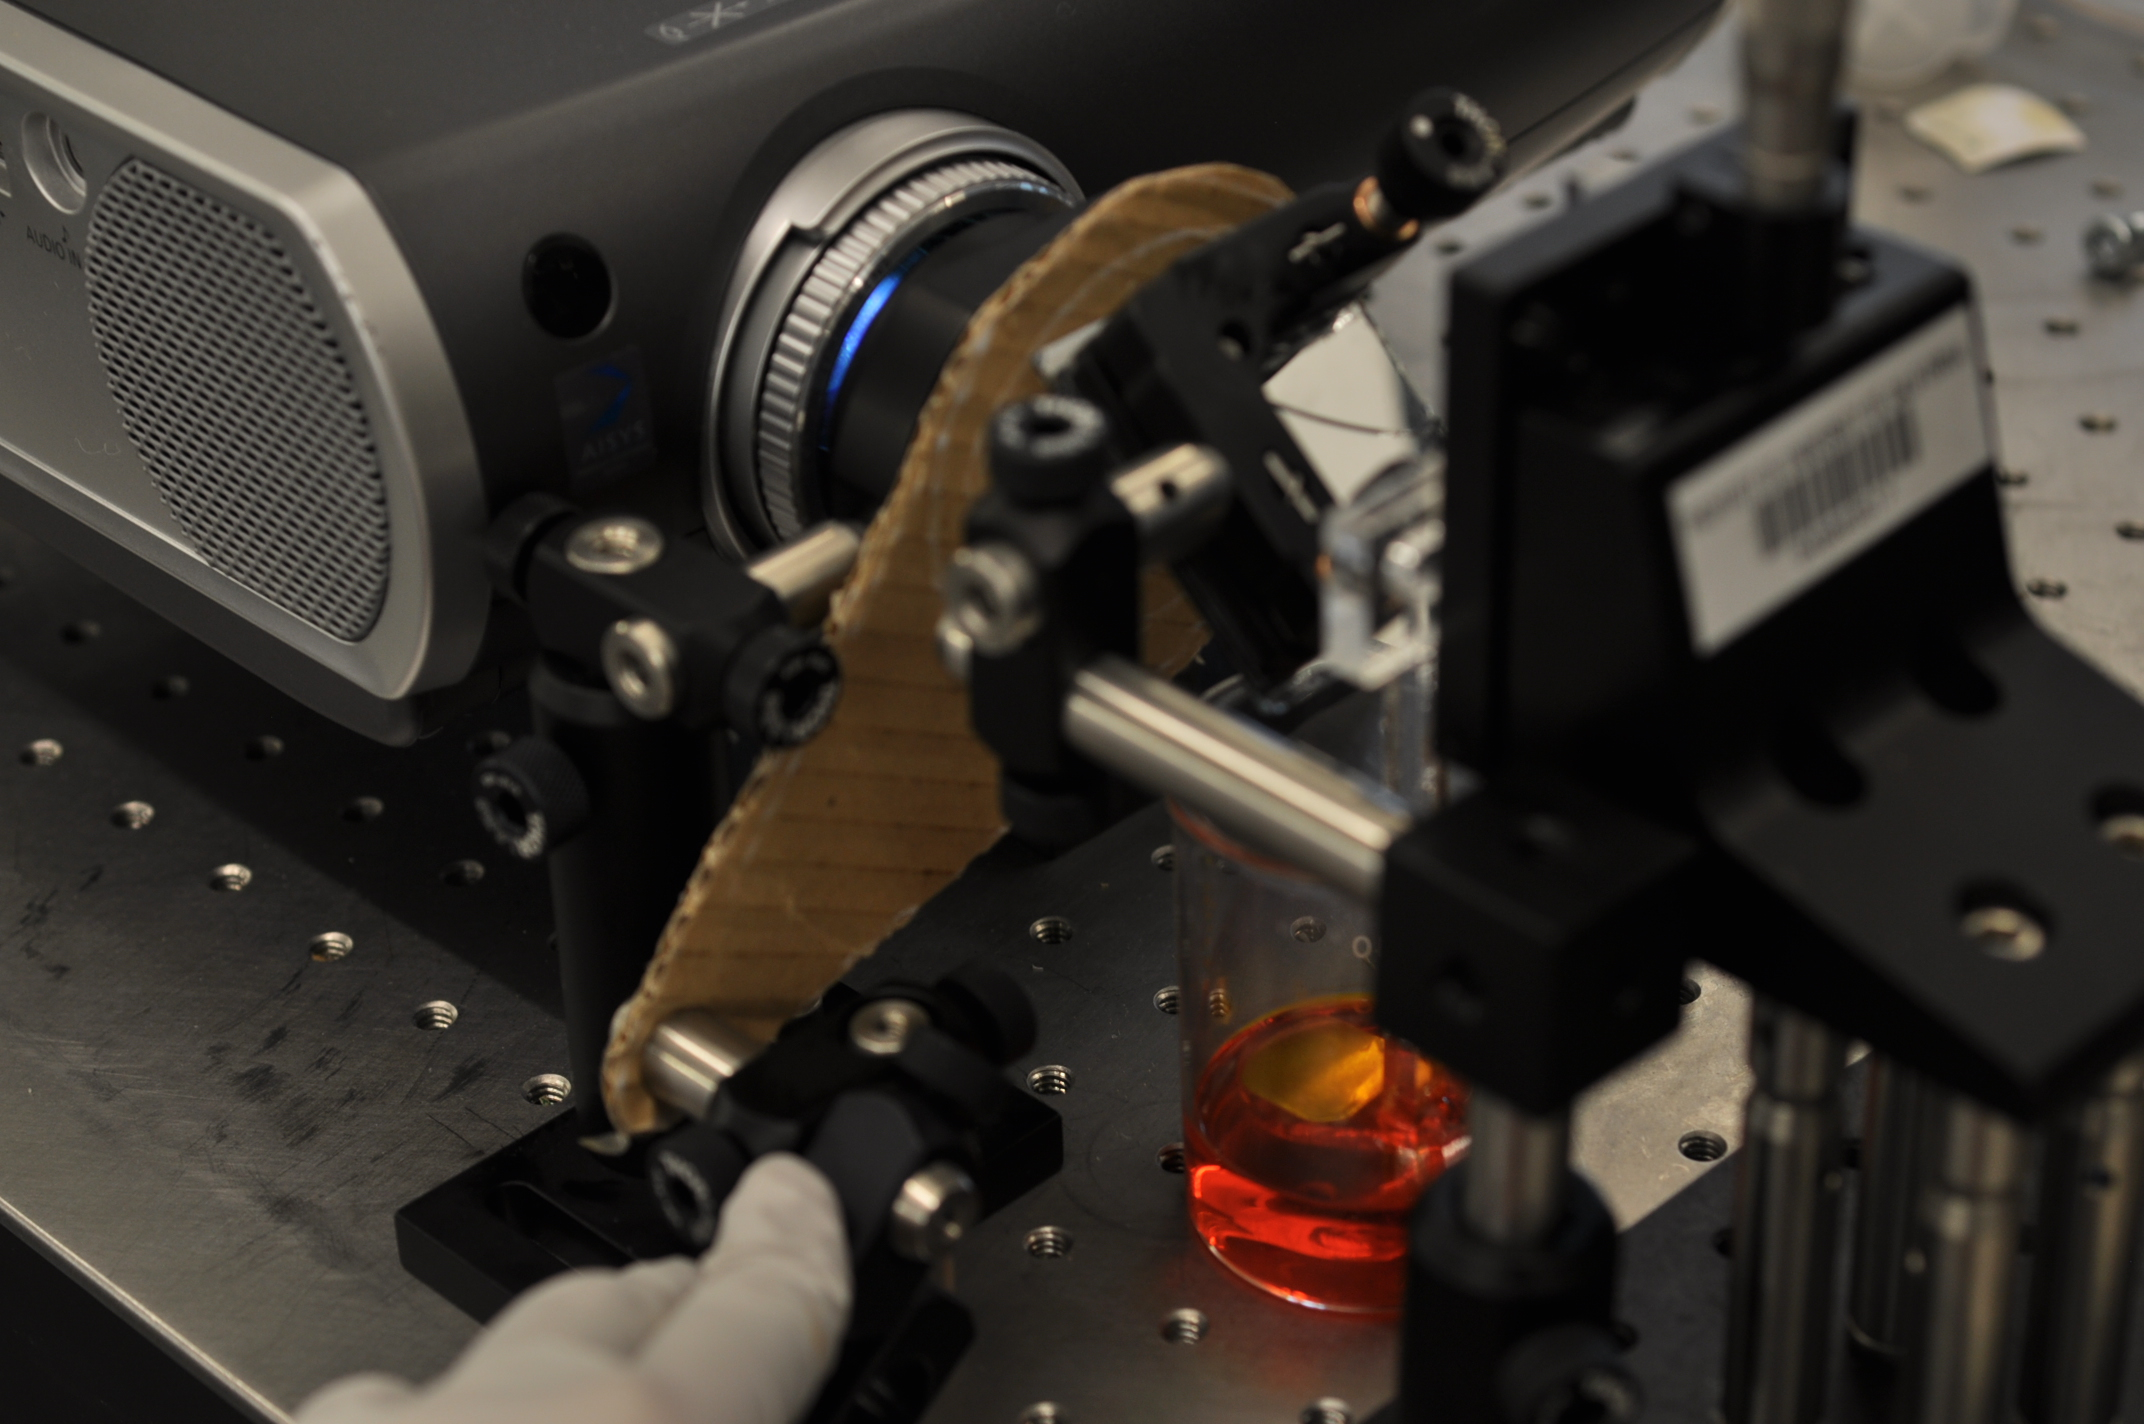
\includegraphics[width=0.3\textwidth]{prt2r.jpg}}\\
		 	\\
		 	\end{tabularx}

		  \begin{tabularx}{\textwidth}{ XXX }
		 	\item \textbf{Step 5} : When hearing 'lower the stage', \textbf{lower} the linear stage. The distance depends on the 
		 	layer height of you sample.
		 	&\raisebox{-\height}{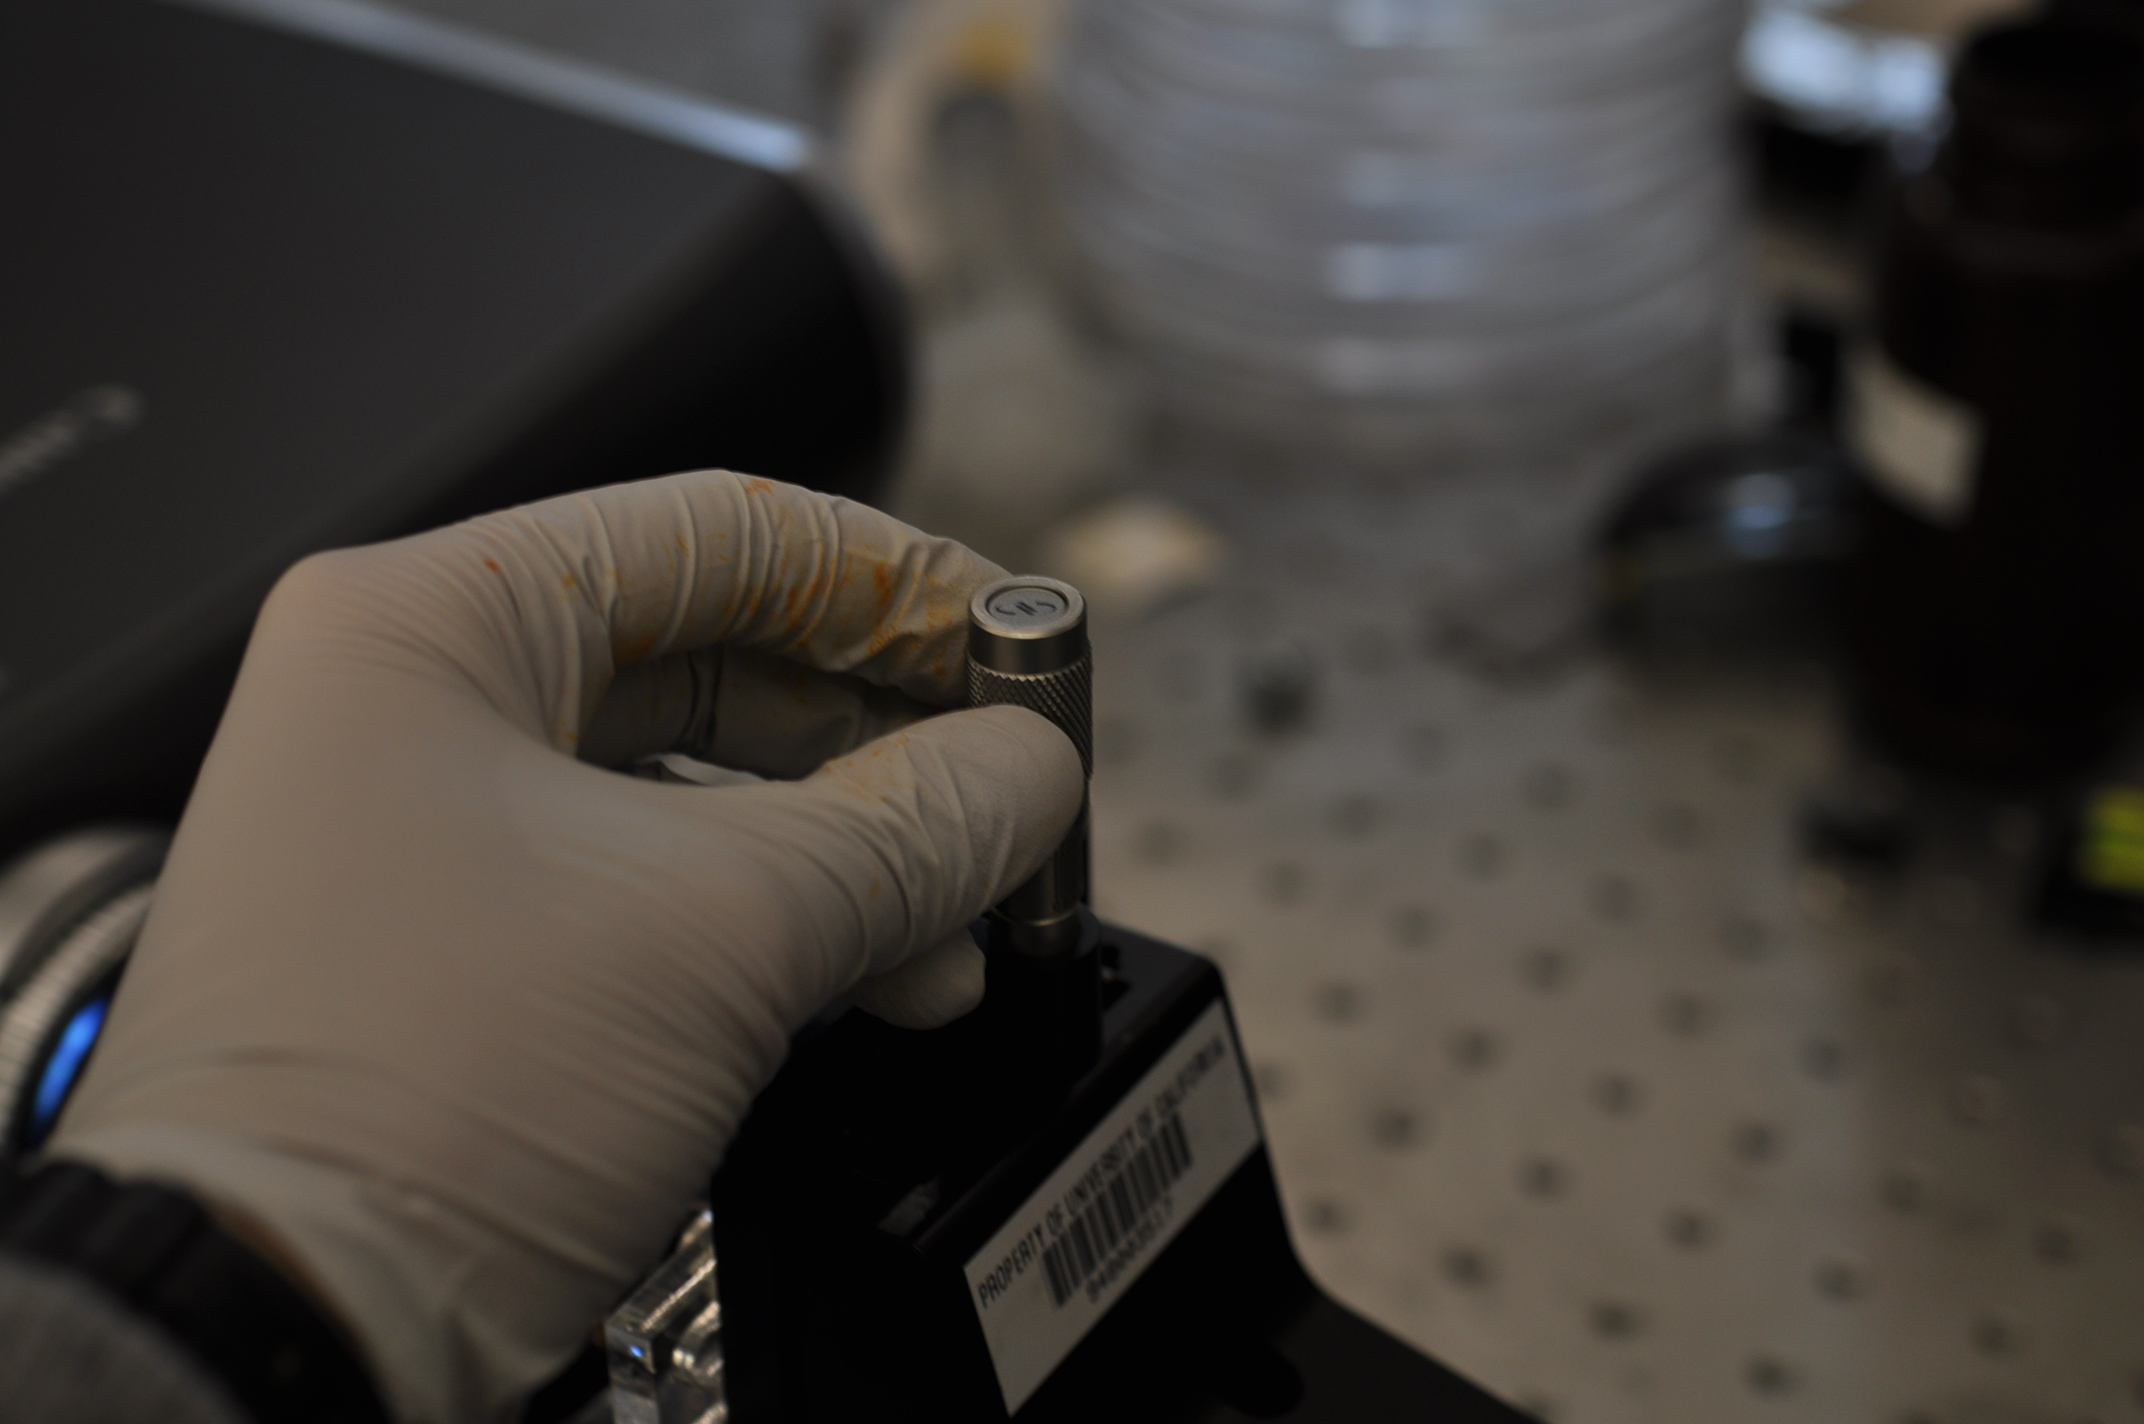
\includegraphics[width=0.3\textwidth]{prt3l.jpg}}
		 	&\raisebox{-\height}{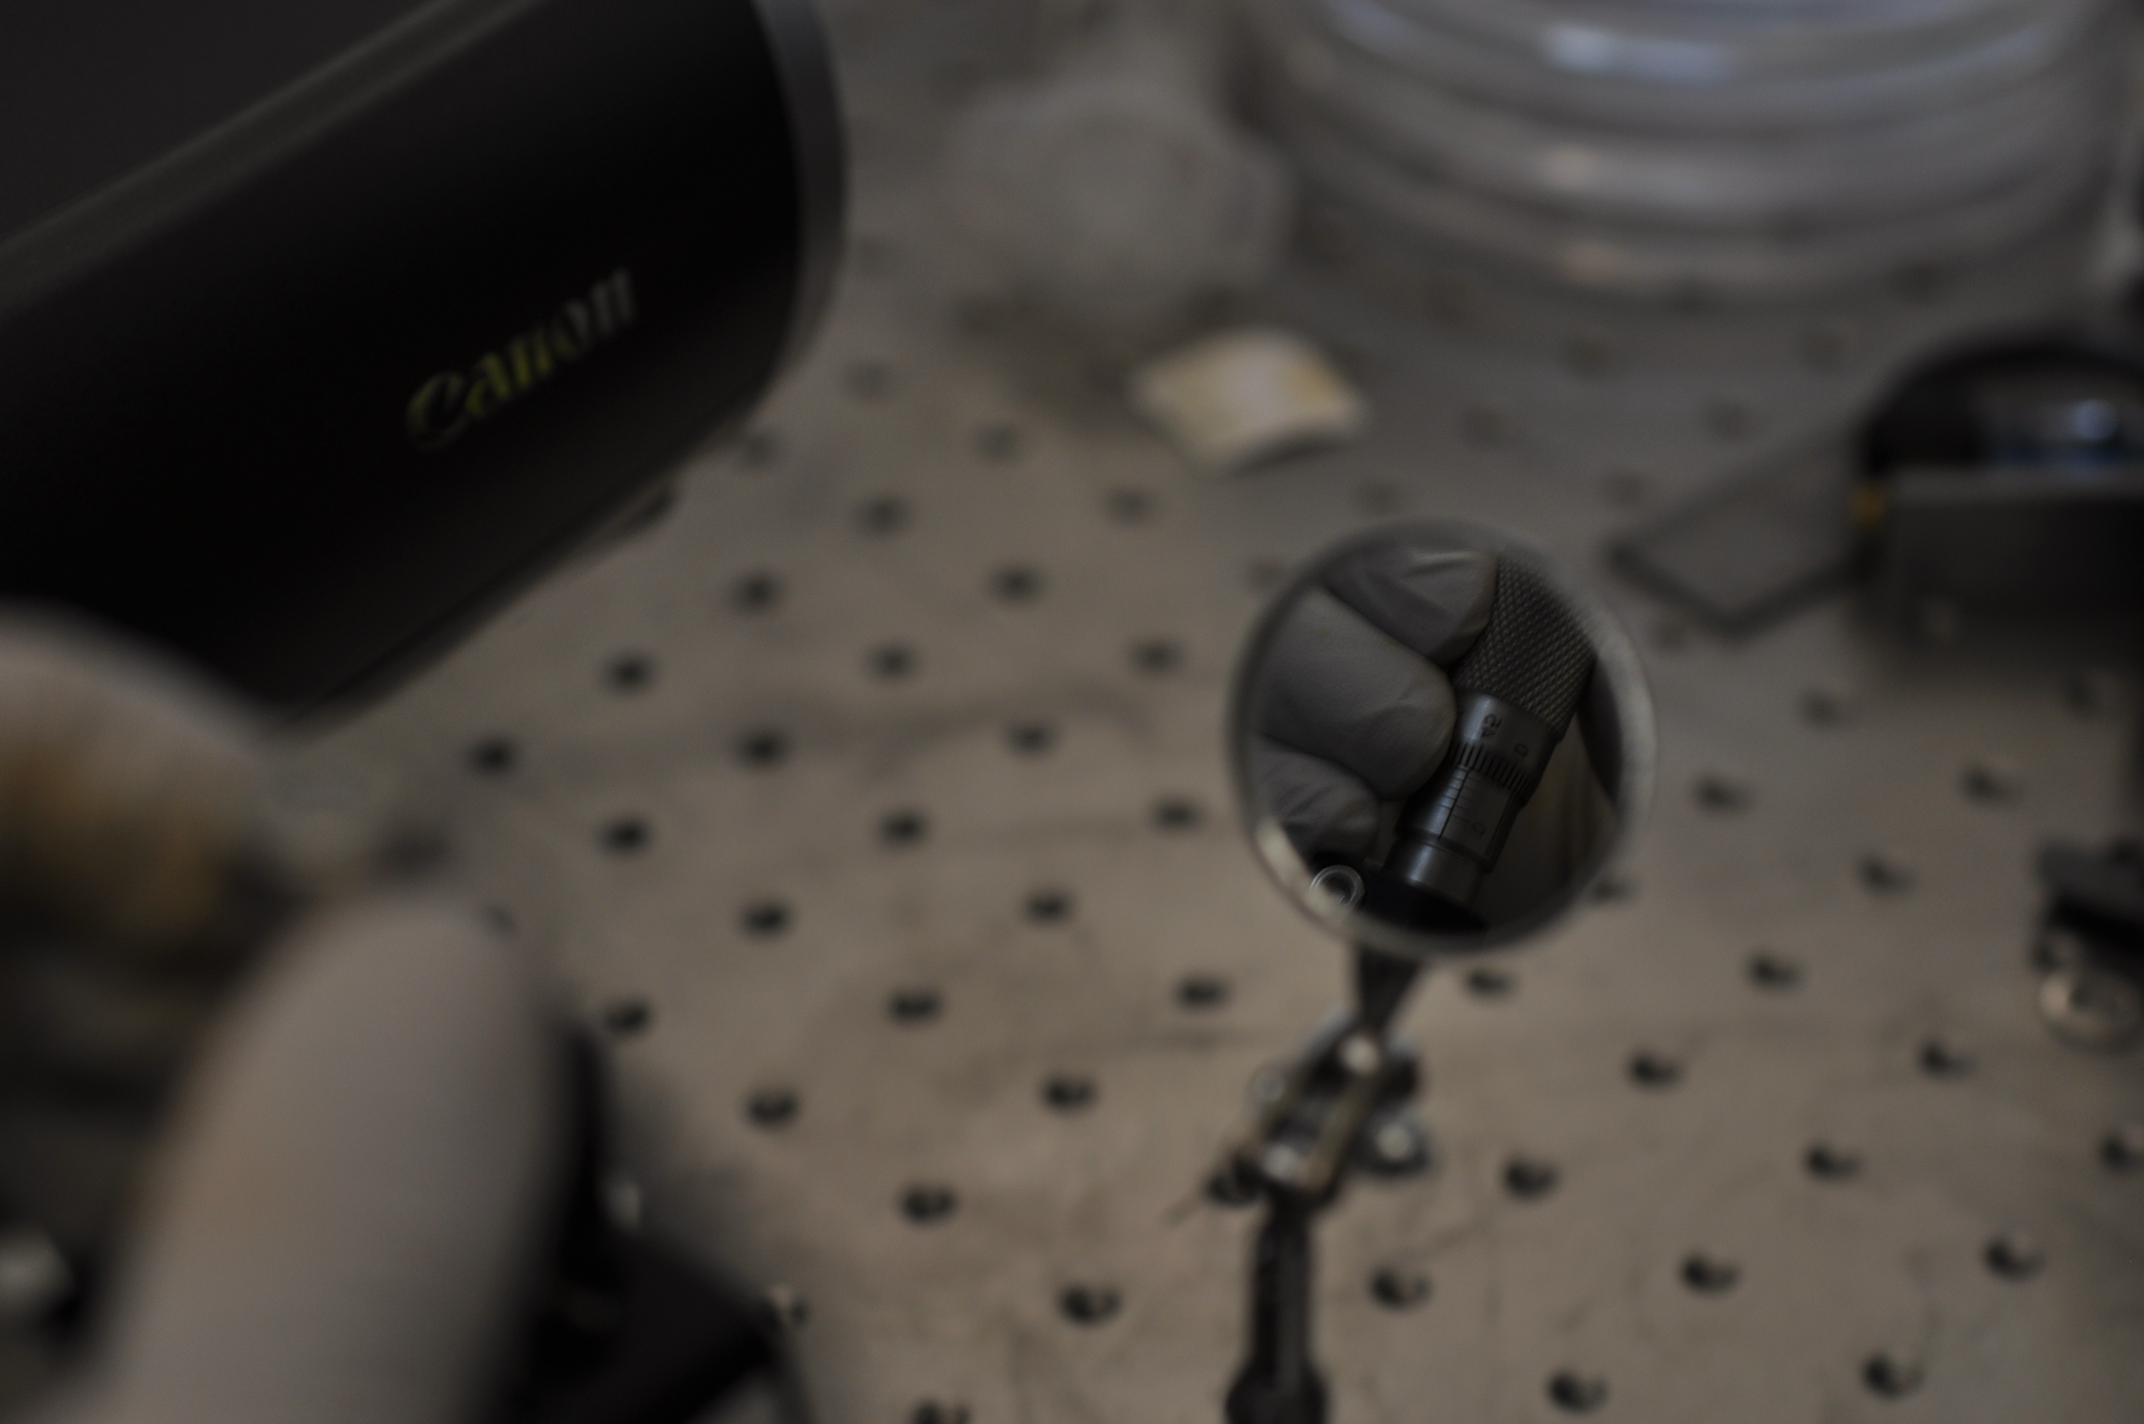
\includegraphics[width=0.3\textwidth]{prt3r.jpg}}\\
		 	\\
		 	\end{tabularx}

		  \begin{tabularx}{\textwidth}{ XXX }
		 	\item \textbf{Step 6} : \textbf{Repeat} step 2 \& 3. When hearing 'Fabrication finish', the sample is done. \textbf{Take away} 
		 	the stage and \textbf{cut} the sample off carefully with a blade.
		 	&\raisebox{-\height}{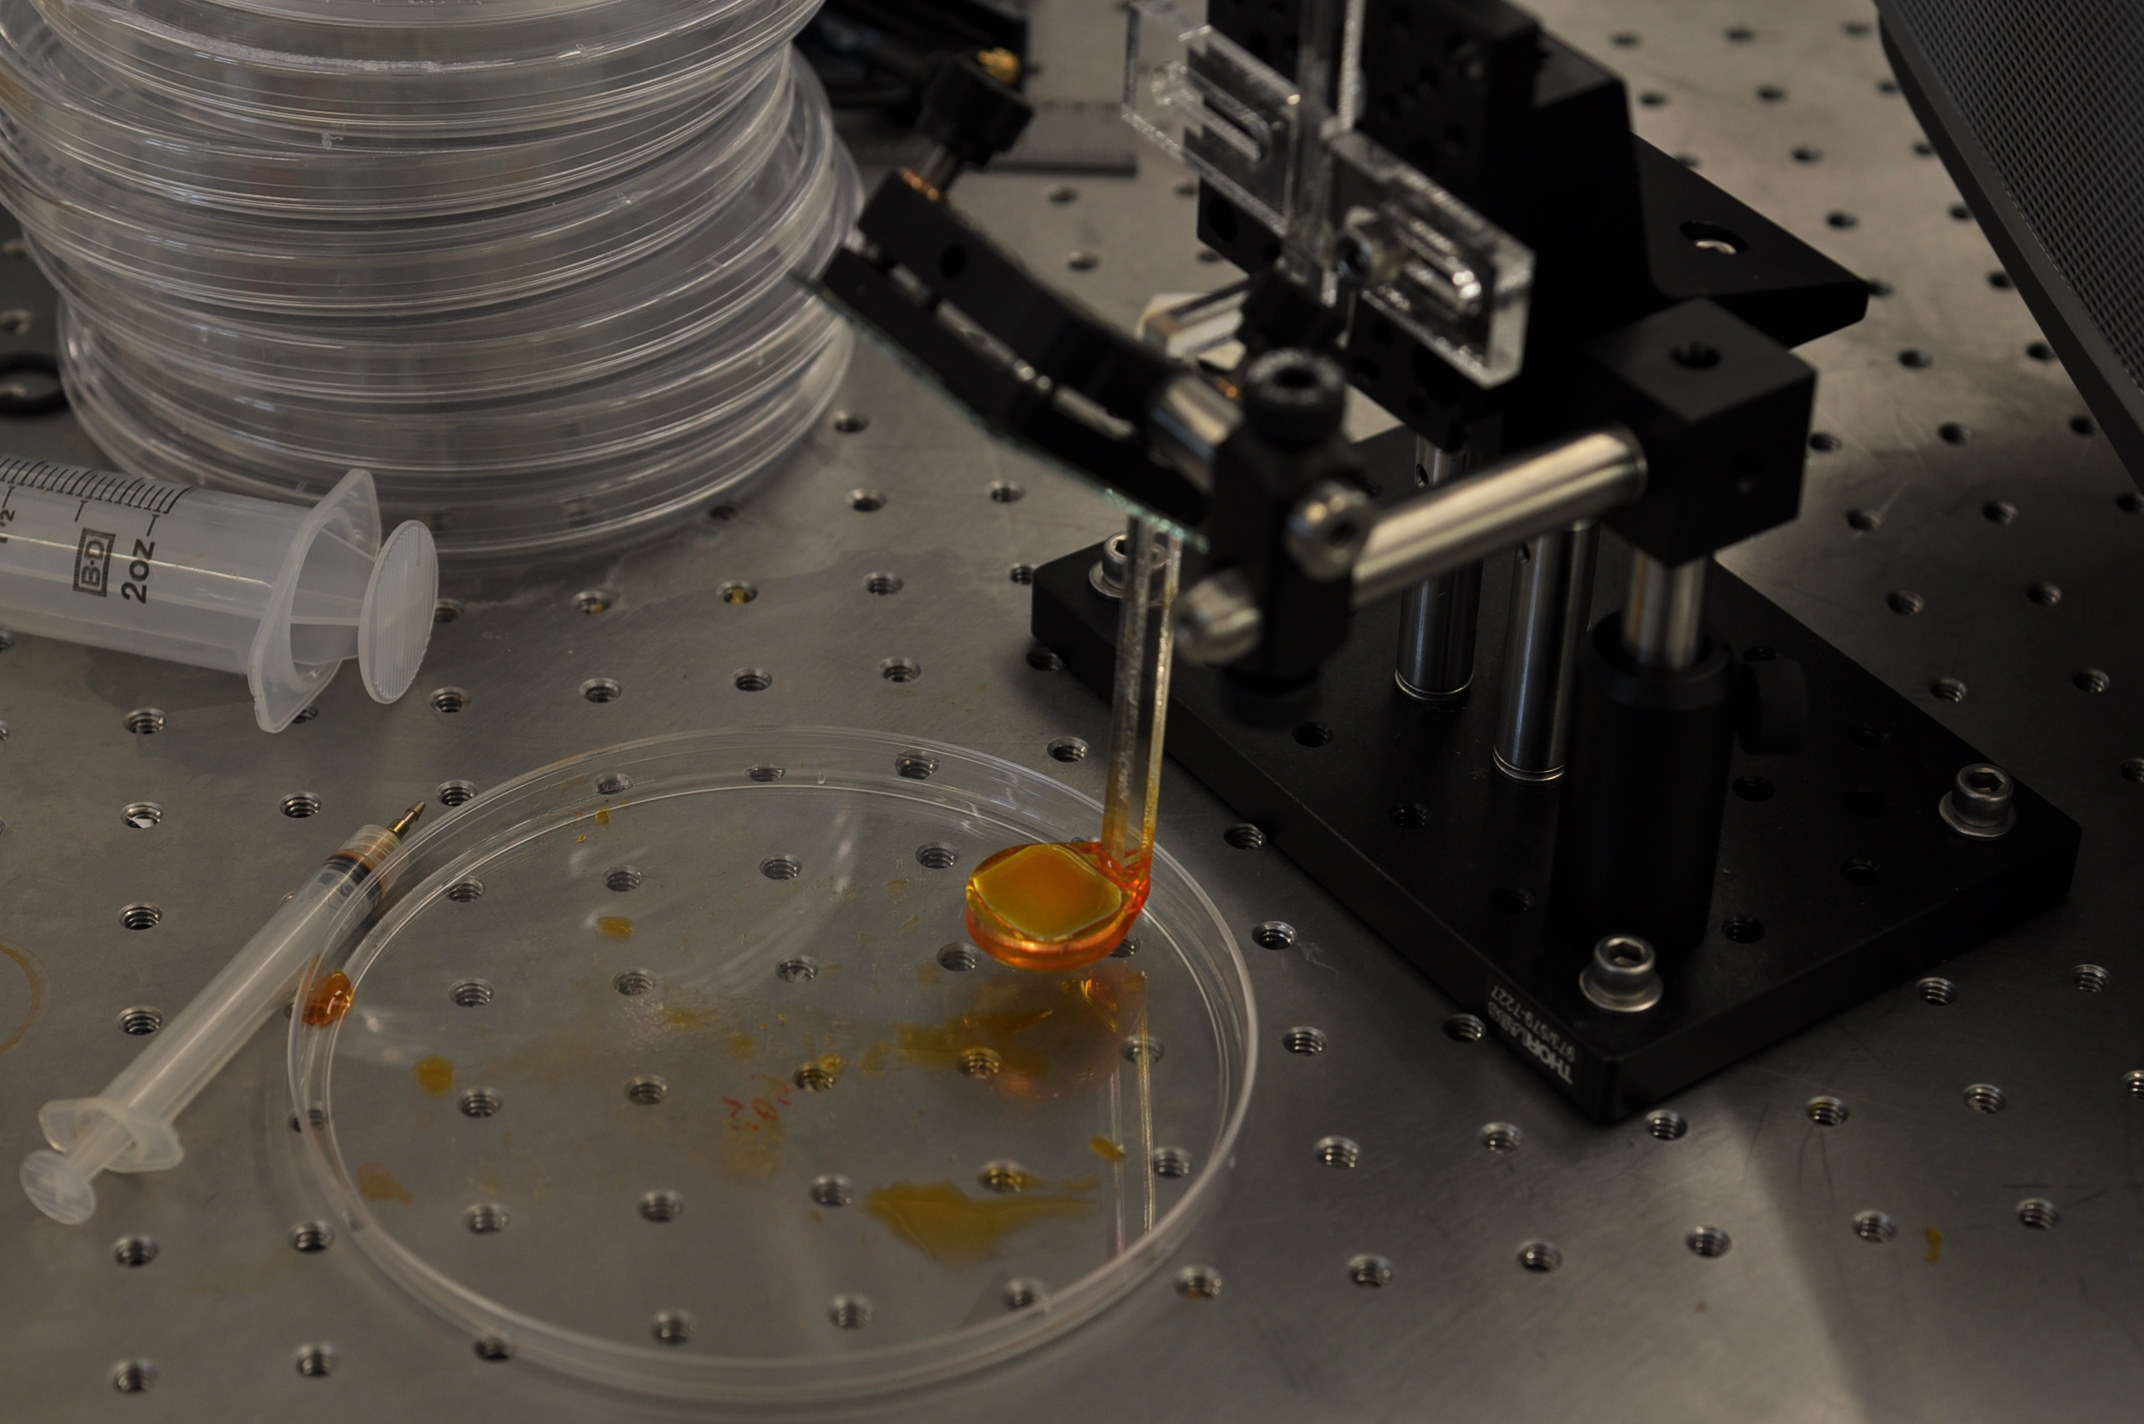
\includegraphics[width=0.3\textwidth]{prt4l.jpg}}
		 	&\raisebox{-\height}{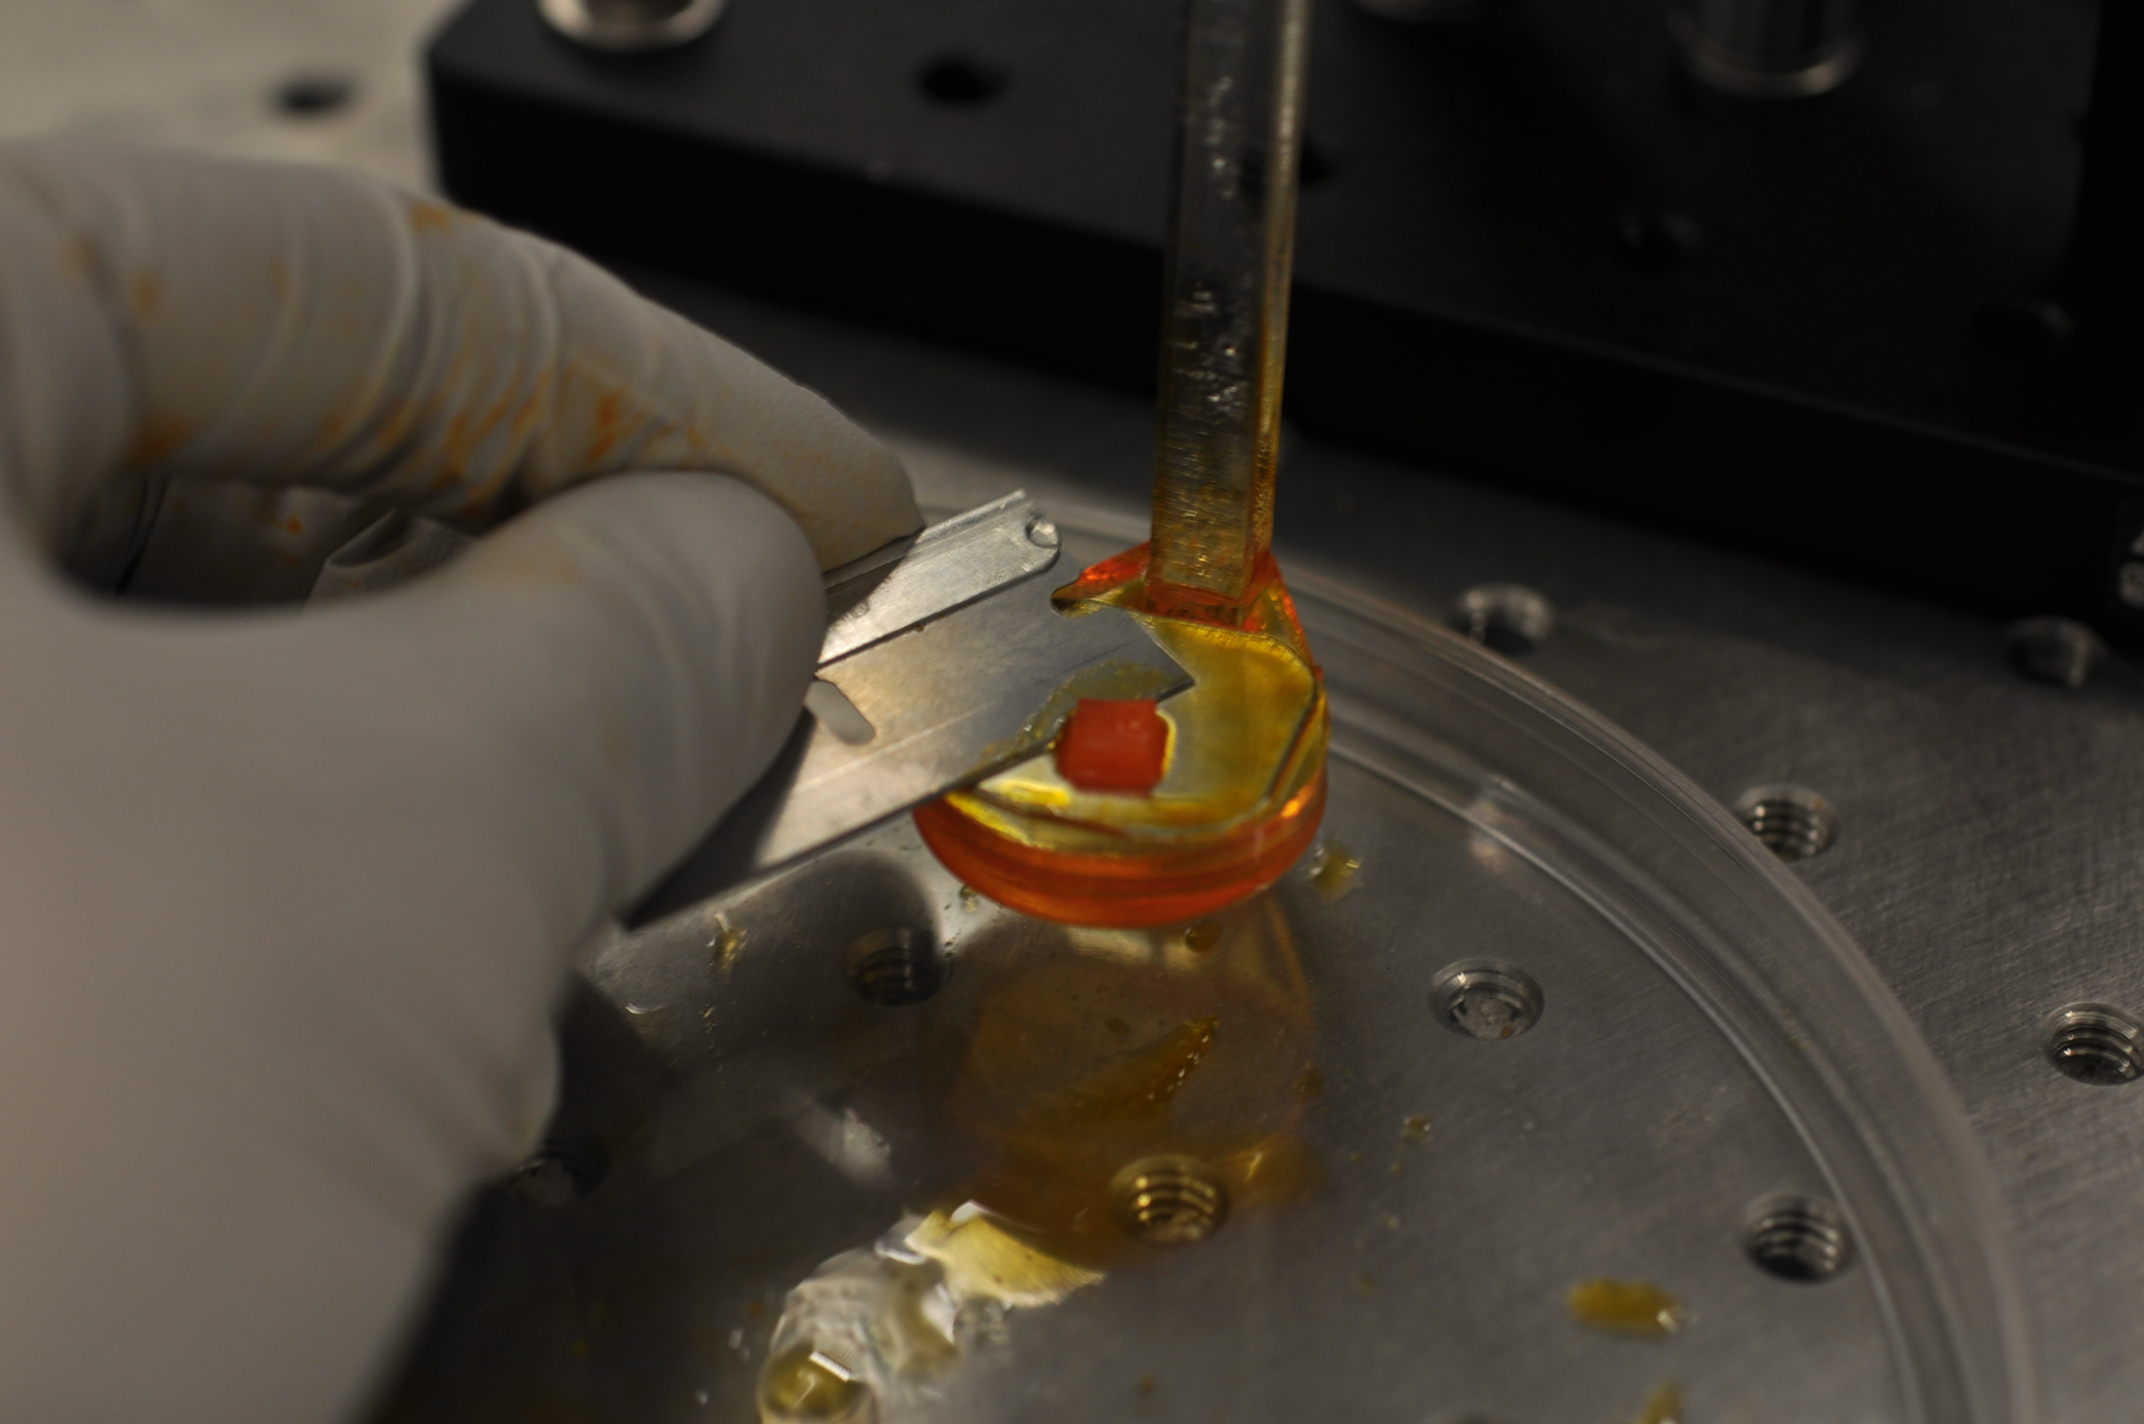
\includegraphics[width=0.3\textwidth]{prt4r.jpg}}\\
		 	\\
		 	\end{tabularx}

		  \begin{tabularx}{\textwidth}{ XXX }
		 	\item \textbf{Step 7} : \textbf{Clean up} the sample holder with isopropanol then \textbf{put} the stage back.
		 	% &\raisebox{-\height}{\includegraphics[width=0.3\textwidth]{prt5l.jpg}}
		 	% &\raisebox{-\height}{\includegraphics[width=0.3\textwidth]{prt5r.jpg}}\\
		  \end{tabularx}
		 \end{itemize}

		% \subsection{Cleaning}\label{sec:cleaning}
		% bla

\end{document}